%%%%%%%%%%%%%%%%%%%%%%%%%%%%%%%%%%%%%%%%%%%%%%%%%%%%%%%%%%%%%%%%%%%%%%%%%%%%%%
% ASU Dissertation Template
%%%%%%%%%%%%%%%%%%%%%%%%%%%%%%%%%%%%%%%%%%%%%%%%%%%%%%%%%%%%%%%%%%%%%%%%%%%%%%
% Copyright 2021 Robert W. Kutter (robert@kutterconsulting.com)
%
%   See also: http://kutterconsulting.com
%
% For guidance on using this file, see the README.
%
%%%%%%%%%%%%%%%%%%%%%%%%%%%%%%%%%%%%%%%%%%%%%%%%%%%%%%%%%%%%%%%%%%%%%%%%%%%%%%
% Preamble
%%%%%%%%%%%%%%%%%%%%%%%%%%%%%%%%%%%%%%%%%%%%%%%%%%%%%%%%%%%%%%%%%%%%%%%%%%%%%%
\newcommand*{\pointsize}{12pt}          %<Set the font size; make sure the size is correct
                                        %   for the font you will use
\documentclass[letterpaper,             % Use US letter-size paper
               oneside,                 % No verso and recto differences
               \pointsize]              % Uses the font size defined above
               {memoir}
\renewcommand{\cleardoublepage}%        % \cleardoublepage will create entirely blank
  {\clearpage}%                         %   pages depending on settings (e.g., usually
                                        %   before start of \mainmatter); redefine it here
                                        %   so that no entirely blank pages are created
                                        %   automatically
%%%%%%%%%%%%%%%%%%%%%%%%%%%%%%%%%%%%%%%
% (Some) Packages
%%%%%%%%%%%%%%%%%%%%%%%%%%%%%%%%%%%%%%%
\usepackage{apacite}
\usepackage{lscape}
\usepackage{booktabs}
\usepackage{rotating}
\usepackage{adjustbox}
\usepackage{graphicx}                   % For importing image files
\usepackage{etoolbox}                   % For advanced commands throughout preamble
\usepackage{microtype}                  %~Improves kerning and protrusion (optional);
                                        %   See here for an introduction:
                                        %   http://www.khirevich.com/latex/microtype/

\providetoggle{usemicrotype}            % TRUE = microtype is being used
\makeatletter                           %   (Used to turn of microtype protrusion in the
\@ifpackageloaded{microtype}%           %   table of contents.)
  {\settoggle{usemicrotype}{true}}%
  {\settoggle{usemicrotype}{false}}
\makeatother
\usepackage{changepage}                 % For changing page layout (e.g., margins) in the
                                        %   middle of the document
\usepackage{calc}					              % Calculate text widths; used in page layout
                                        %   changes

%%%%%%%%%%%%%%%%%%%%%%%%%%%%%%%%%%%%%%%
% Title page, input
%%%%%%%%%%%%%%%%%%%%%%%%%%%%%%%%%%%%%%%
\listadd{\titlelines}%
  {Fostering Collaborative Solutions in the Opioid Overdose Crisis: Law Enforcement as a Potential Partner in Reducing Fatalities}             %<Enter the title of the dissertation
%\listadd{\titlelines}%
%  {Second Line of the Title}            % If you want to
                                        %   split the title across lines,
                                        %   use another \listadd command for the
                                        %   second line
\newcommand*\Author{Seth Watts}          %<Enter your name; must match official transcript
\newcommand*{\documentname}%
  {Dissertation}                        %<Enter the type of document (capitalized)
\newcommand*{\degreename}
  {Doctor of Philosophy}                %<Enter the type of degree (capitalized)
\newcommand*\defdate{November 2024}        %<Give month (written out fully) and year of
                                        %   the oral defense
\listadd{\committeechair}{Michael D. White}   %<Enter committee chair name; use \listadd for
%\listadd{\committeechair}{Another name}%   for additional names
\newcommand*{\chairlabel}{Chair}        %<If you have co-chairs, replace this text with
                                        %   'Co-Chair'
\listadd{\committeemember}{Jacob T. N. Young} %<Enter committee member names; use \listadd for
\listadd{\committeemember}{Alyssa W. Chamberlain}
\listadd{\committeemember}{Brandon del Pozo}%   additional names
\newcommand*{\gradmonth}{December}         %<Enter the graduation date; month can only be:
                                        %  May, August, or December
\newcommand*{\gradyear}{2024}           %<Enter the graduation year, e.g. 2014

\listadd{\keywords}{Police}          %<Enter keywords; use \listadd for
\listadd{\keywords}{Public Health}
\listadd{\keywords}{Opioids}%   additional names (up to 6)
\newcommand*{\graddate}{\gradmonth%     % Compose full graduation date
  \space\gradyear}

%%%%%%%%%%%%%%%%%%%%%%%%%%%%%%%%%%%%%%%
% Page layout
%%%%%%%%%%%%%%%%%%%%%%%%%%%%%%%%%%%%%%%
\settrimmedsize{\stockheight}%          % Specifies \paperheight and \paperwidth
  {\stockwidth}{*}
\settrims{0pt}{0pt}                     % Set location of page in relation to the stock.
                                        % Paper and stock size are equivalent,
                                        % so both \trimtop and \trimedge are set to 0pt
\newlength{\forfootskip}
\setlength{\forfootskip}%
  {3\baselineskip}
\newlength{\textblockheight}            % Calculate height of text block to leave room
\setlength{\textblockheight}{9.0in}     %   for footers, keeping page numbers outside
\addtolength{\textblockheight}%         %   the 1in vertical margins
  {-\forfootskip}
\settypeblocksize{\textblockheight}%    % Calculated by 1.0in vertical margins and
  {*}{*}                                %   letting margins set the width of the typeblock
\setulmargins{1.0in}{*}{*}              % Set upper margin (\uppermargin, not \topmargin);
                                        %   calculate the bottom margin
\setlrmarginsandblock{1.25in}{1.25in}{*}%~Set margins and calculate width of typeblock
\setheaderspaces{*}{0.5\baselineskip}{*}% Arguments: '\headdrop', '\headsep', and/or ratio
                                        %   Note: This is only used in the list of
                                        %   contents sections
\setheadfoot{\baselineskip}%            % Set '\headheight' and '\footskip'
  {\forfootskip}
\checkandfixthelayout                   % Required by memoir package after setting layout
\settypeoutlayoutunit{in}               % Write layout dimensions to log file in inches

%%%%%%%%%%%%%%%%%%%%%%%%%%%%%%%%%%%%%%%
% Fonts
%%%%%%%%%%%%%%%%%%%%%%%%%%%%%%%%%%%%%%%
\usepackage[T1]{fontenc}                % Standard option to handle, e.g., accented
                                        %   characters like 'ö' better
\usepackage{amssymb,mathtools}          % For AMS-LaTeX, see here for more:
                                        %     http://www.ams.org/publications/authors/tex/amslatex
                                        % ('mathtools' loads and extends 'amsmath')
\usepackage{ifxetex,ifluatex}           % Can check if XeTeX or LuaTeX was used to typeset
\usepackage{fixltx2e}                   % Provides \textsubscript
\IfFileExists{upquote.sty}%             % Use upquote if available, for
  {\usepackage{upquote}}{}              %   straight quotes in verbatim environments

% Load fonts depending on the
%   typesetting engine
\ifnum 0\ifxetex 1\fi\ifluatex 1\fi=0   % If pdftex
  \usepackage[utf8]{inputenc}           %   'utf8' should match the encoding of this file
                                        %
                                        %~Set up your font in pdftex here
                                        %
\else 									                % If xetex or luatex
  \ifxetex                              % If xetex
    \usepackage{mathspec}               % Matches non-math open-type font to math
                                        %   open-type font (use 'mathspec' if you want to
                                        %   write math in unicode)
    \usepackage{xunicode}               % Convert LaTeX character macros to unicode
  \else                                 % If luatex\usepackage{fontspec}
    \usepackage{fontspec}               % Use fontspec for (open type) font selection
  \fi
  \defaultfontfeatures{Mapping=tex-text,% Font spec setting
    Scale=MatchLowercase}
  \newcommand*{\euro}{€}

  % Using fonts in XeLaTeX can be complicated; the following settings
  % work when this file is compiled inside the Docker container produced
  % by the `build.sh` script.
  %
  % Sometimes something simple like the following will work:
  %
  %   \setmainfont{Garamond}
  %
  % But often the easiest solution is to move font files (*.otf or *.ttf) into
  % a sub-directory and provide the direct path to them here.
  %
  % See `fontspec` documentation for more on using local font files.
  %
  \setmainfont{EBGaramond12}[           %<Set the main font; make sure the font is correct
                                        %   for the font size (See ASU Style Guide)
    Path          = /usr/share/fonts/opentype/ebgaramond/,
    Extension     = .otf ,
    UprightFont   = *-Regular ,
    ItalicFont    = *-Italic ,
    % Notice that bold is missing here because the Docker image does not have
    % a bold typeface for Garamond; it would probably be possible to find
    % one on your local system or online.
  ]

%  \setmathfont(Digits,Latin,Greek)%     %~Uncomment two lines to set a font for math%
%    {MATHFONT}
\fi

%%%%%%%%%%%%%%%%%%%%%%%%%%%%%%%%%%%%%%%
% Line spacing
%%%%%%%%%%%%%%%%%%%%%%%%%%%%%%%%%%%%%%%
\DoubleSpacing                          % True double spacing
\BeforeBeginEnvironment{quote}          % Memoir leaves most special material
  {\par\SingleSpacing}                  %   single spaced, but makes block quotes
\AfterEndEnvironment{quote}%            %   double-spaced; fix to follow ASU style guide
  {\vspace{-\baselineskip} %
  \DoubleSpacing}
\BeforeBeginEnvironment{quotation}%
  {\par\SingleSpacing}
\AfterEndEnvironment{quotation}%
  {\vspace{-\baselineskip} %
  \DoubleSpacing}

\setlength{\footnotesep}{\baselineskip} % Double space *between* footnotes
\renewcommand*{\footnoterule}{%         % Redefine footnoterule so that initial footnote
  \kern-3pt%                            %   still appears right under the rule (changing
  \hrule width 0.4\columnwidth          %   \footnotesep also changes the space between the
  \kern 2.6pt                           %   rule and the first footnote
  \vspace{-0.5\baselineskip}            % (Here is the vertical space adjustment)
  }

\usepackage{enumitem}                   % Control spacing in enumerate environment
\setlist{noitemsep}                     % Remove extra vertical spacing between items in lists
                                        % \setlist{nosep} to leave no space around whole list

%%%%%%%%%%%%%%%%%%%%%%%%%%%%%%%%%%%%%%%
% Page numbering
%%%%%%%%%%%%%%%%%%%%%%%%%%%%%%%%%%%%%%%
\makepagestyle{ASU}
  \makeevenfoot{ASU}{}{\thepage}{}
  \makeoddfoot{ASU}{}{\thepage}{}

%%%%%%%%%%%%%%%%%%%%%%%%%%%%%%%%%%%%%%%
% Title page, formatting
%%%%%%%%%%%%%%%%%%%%%%%%%%%%%%%%%%%%%%%
\newlength{\savedfootskip}
\setlength{\savedfootskip}{\footskip}
\newcommand{\titlepagesetup}{%          % Page layout for title page
  \changepage%                          % Adjustment to page dimensions:
    {\savedfootskip}%                   %   text height
    {}%                                 %   text width
    {}%                                 %   even-side margin
    {}%                                 %   odd-side margin
    {}%                                 %   column sep.
    {}%                                 %   topmargin
    {}%                                 %   headheight
    {}%                                 %   headsep
    {-\savedfootskip}%                  %   footskip
}

\newcommand{\closetitlepagesetup}{%     % Undo set up for title page
  \changepage{-\savedfootskip}{}{}{}{}%
    {}{}{}{\savedfootskip}%
}

\makeatletter                           % Do not modify this section; Enter info above
\newcommand*{\titlepageASU}{
  \titlepagesetup
  \clearpage
  \begin{center}
  \SingleSpacing
  \thispagestyle{empty}
    \renewcommand*{\do}[1]{##1 \\[\baselineskip]}
    \dolistloop{\titlelines}
    by \\[\baselineskip]
    \Author \\[5\baselineskip]
    A \documentname~Presented in Partial Fulfillment \\
    of the Requirements for the Degree \\
    \degreename \\
    \vfill                              % Vertically center the portion below
    Approved \defdate~by the \\
    Graduate Supervisory Committee: \\[\baselineskip]
    \renewcommand*{\do}[1]{##1, \chairlabel \\}
    \dolistloop{\committeechair}
    \renewcommand*{\do}[1]{##1 \\}
    \dolistloop{\committeemember}
    \vfill                              % Vertically center the portion above
    ARIZONA STATE UNIVERSITY \\[\baselineskip]
    \graddate
  \end{center}
  \clearpage
  \closetitlepagesetup
}
\makeatother

%%%%%%%%%%%%%%%%%%%%%%%%%%%%%%%%%%%%%%%
% Heading styles
%%%%%%%%%%%%%%%%%%%%%%%%%%%%%%%%%%%%%%%
% Note: memoir also has \book and \part commands; do not use these
\makechapterstyle{ASU}{%                % Define chapter heading style
  \renewcommand*{\chapterheadstart}{}   % Chapter title flush with top margin
  \renewcommand*{\chapnamefont}%        % Set font for 'Chapter' or 'Appendix'
    {\normalfont}
  \renewcommand*{\chapnumfont}%         % Set font for number in chapter headings
    {\normalfont}
  \renewcommand*{\afterchapternum}%     % Insert a double line break after
    {\\[\baselineskip]}                 %   chapter number
  \renewcommand*{\chaptitlefont}%       % Set font for chapter title name
    {\normalfont}
  \setlength{\afterchapskip}{0pt}       % Set vertical space between chapter title and
                                        %   first paragraph; equivalent to one line break
                                        %   (vertical space = \afterchapskip + \baselineskip)
                                        % Note: This \afterchapskip value is only used in
                                        %   front matter
  \renewcommand*{\printchapternum}{%    % Center justify chapter number
    \centering \chapnumfont %
    \thechapter}
  \renewcommand*{\printchaptertitle}[1]%% Center justify
    {\expandafter\centering %           %   \MakeUppercase has issues; see here for some
    \expandafter\chaptitlefont %        %   details: https://tex.stackexchange.com/questions/35680/uppercase-in-newcommand
    \expandafter\MakeUppercase %        %   Accented characters and some fonts may not
    \expandafter{##1}}                  %   uppercase correctly; if that happens, just
                                        %   type the chapter title in uppercase
}

\setsecnumdepth{all}                    %~Enter the levels that you want to have numbered
                                        %   (Default is to number all [5 levels deep].)

\newcommand{\divisionbeforeskip}%       % Create default formatting for headings
  {\baselineskip}
\newcommand{\divisionindent}%
  {0.5em}
\newcommand{\divisionfont}{\normalfont} % Font must be \normalfont
\newcommand{\divisionafterskip}%
  {\baselineskip}

\setbeforesecskip{\divisionbeforeskip}  % Apply default formatting to all heading levels
\setsecindent{\divisionindent}          % Note: If you change \setsecnumdepth above, you
\setsecheadstyle{\divisionfont}         %   will need to set the indent for all lower
\setaftersecskip{\divisionafterskip}    %   levels to '0pt'; otherwise, they will be
                                        %   preceded by unnecessary space
\setbeforesubsecskip{\divisionbeforeskip}
\setsubsecindent{\divisionindent}
\setsubsecheadstyle{\divisionfont}
\setaftersubsecskip{\divisionafterskip}

\setbeforesubsubsecskip{\divisionbeforeskip}
\setsubsubsecindent{\divisionindent}
\setsubsubsecheadstyle{\divisionfont}
\setaftersubsubsecskip{\divisionafterskip}

\setbeforeparaskip{\divisionbeforeskip}
\setparaindent{\divisionindent}
\setparaheadstyle{\divisionfont}
\setafterparaskip{\divisionafterskip}

\setbeforesubparaskip{\divisionbeforeskip}
\setsubparaindent{\divisionindent}
\setsubparaheadstyle{\divisionfont}
\setaftersubparaskip{\divisionafterskip}

%%%%%%%%%%%%%%%%%%%%%%%%%%%%%%%%%%%%%%%
% Paragraph formatting
%%%%%%%%%%%%%%%%%%%%%%%%%%%%%%%%%%%%%%%
%\sloppybottom                          % Reduce the chances of widows
\raggedbottom                           % Loosens vertical spacing requirements, so
                                        %   \sloppybottom doesn't make pages look bad;
                                        %   it also prevents large gaps in the middle of
                                        %   pages and pushes them to the bottom of pages
\indentafterchapter                     % Overrides the default which is not to indent
                                        %   the first paragraph in a chapter, but it
                                        %   looks odd in some places to not indent
                                        %   paragraphs

%%% List Titles %%%
\renewcommand{\contentsname}%           % Set heading for each list
  {Table of Contents}%                  %   Formatted as chapter headings by default, so
\renewcommand{\listtablename}%          %   no additional heading formatting is needed
  {List of Tables}
\renewcommand{\listfigurename}%
  {List of Figures}

%%% Depth %%%
\settocdepth{subparagraph}              % Include 5 levels deep (all levels) in TOC

%%% Fonts %%%
\makeatletter%
\patchcmd{\l@part}%                     % Patch the command that writes part-level entries
    {\cftpartfont {#1}}%                %   to the table of contents, so they are in
    {\normalfont \texorpdfstring{%      %   'normalfont' and uppercase
      \uppercase{#1}}{{#1}} }%
    {\typeout{Success: Patch %
      'l@part' to uppercase %
      part-level headings in the %
      table of contents.}}%
    {\typeout{Fail: Patch %
      'l@part' to uppercase %
      part-level headings in the %
      table of contents.}}%
\makeatother%

\makeatletter%
\patchcmd{\l@chapapp}%                  % Patch the command that writes chapter-level
    {\cftchapterfont {#1}}%             %   entries to the table of contents, so they are
    {\normalfont \texorpdfstring{%      %   in 'normalfont' and uppercase
      \uppercase{#1}}{{#1}} }%
    {\typeout{Success: Patch %
      'l@chapapp' to uppercase %
      part-level headings in the %
      table of contents.}}%
    {\typeout{Fail: Patch %
      'l@chapapp' to uppercase %
      part-level headings in the %
      table of contents.}}%
\makeatother%

% If not using 'hyperref', use the following commands to adjust 'part' and 'chapter'
%   level headings in the TOC
%\renewcommand*{\cftpartfont}%          % Uppercase 'part' and 'chapter' headings
%  {\normalfont\MakeTextUppercase}      % Note: Sending \MakeTextUppercase to the TOC
%\renewcommand*{\cftchapterfont}%       %   conflicts with hyperref and breaks it!
%  {\normalfont\MakeTextUppercase}%

\usepackage{titlecaps}                  % Set up headline style for captions in the
                                        %   lists of tables and figures
                                        % Note: ASU style guide does not provide
                                        %   comprehensive guidelines for headlines, so
                                        %   Chicago style for headline style is used
                                        % Note: Last word in title is not explicitly
                                        %   capitalized; in general, these settings are
                                        %   broadly correct, but captions should be
                                        %   reviewed to ensure they are being capitalized
                                        %   properly
\Resetlcwords
\Addlcwords{a an the}                   % Leave articles lowercase
\Addlcwords{and but for or nor}         % Leave conjunctions lowercase
\Addlcwords{aboard about above across % % Leave all prepositions lowercase
  after against along amid among anti % %   (This is a [non-exhaustive] list of common
  around as at before behind below %    %   one-word prepositions)
  beneath beside besides between %
  beyond but by concerning considering %
  despite down during except excepting %
  excluding following for from in %
  inside into like minus near of off %
  on onto opposite outside over past %
  per plus regarding round save since %
  than through to toward towards under %
  underneath unlike until up upon %
  versus vs via with within without}
\Addlcwords{ according\space{to} %      % Leave two-word conjunctions lowercase
  ahead\space{of} apart\space{from} %   %   (This is a [non-exhaustive] list of common
  as\space{for} as\space{of} %          %   two-word prepositions.)
  as\space{per} as\space{regards} %
  aside\space{from} astern\space{of} %
  back\space{to} because\space{of} %
  close\space{to} due\space{to} %
  except\space{for} far\space{from} %
  in\space{to} inside\space{of} %
  instead\space{of} left\space{of} %
  near\space{to} next\space{to} %
  on\space{to} opposite\space{of} %
  opposite\space{to} out\space{from} %
  out\space{of} outside\space{of} %
  owing\space{to} prior\space{to} %
  pursuant\space{to} rather\space{than} %
  regardless\space{of} right\space{of} %
  subsequent\space{to} such\space{as} %
  thanks\space{to} that\space{of} %
  up\space{to}}

\renewcommand{\cfttableaftersnumb}%     % Put table captions in List of Tables in title
  {\titlecap}%                          %   case
\renewcommand{\cftfigureaftersnumb}%    % Put table captions in List of Figures in title
  {\titlecap}%                          %   case

\renewcommand*{\cftpartpagefont}%       % Use normal font for all page numbers
  {\normalfont}
\renewcommand*{\cftchapterpagefont}%
  {\normalfont}
\renewcommand*{\cftsectionpagefont}%
  {\normalfont}
\renewcommand*{\cftsubsectionpagefont}%
  {\normalfont}
\renewcommand*{\cftsubsubsectionpagefont}%
  {\normalfont}
\renewcommand*{\cftsubsubsectionpagefont}%
  {\normalfont}
\renewcommand*{\cftparagraphpagefont}%
  {\normalfont}
\renewcommand*{\cftsubparagraphpagefont}%
  {\normalfont}
\renewcommand*{\cftfigurepagefont}%
  {\normalfont}
\renewcommand*{\cfttablepagefont}%
  {\normalfont}

\cftpagenumbersoff{part}                % Turn off page numbers for 'part's, which are
                                        %   actually serving as headings within the TOC

%%% Vertical Space %%%
\setlength{\cftbeforepartskip}{0pt}     % Remove all additional vertical spacing so TOC
\setlength{\cftbeforechapterskip}{0pt}  %   is double spaced uniformly
\setlength{\cftbeforesectionskip}{0pt}
\setlength{\cftbeforesubsectionskip}{0pt}
\setlength{\cftbeforesubsubsectionskip}{0pt}
\setlength{\cftbeforeparagraphskip}{0pt}
\setlength{\cftbeforesubparagraphskip}{0pt}
\setlength{\cftbeforefigureskip}{0pt}
\setlength{\cftbeforetableskip}{0pt}

\renewcommand{\insertchapterspace}{%    % By default, extra vertical space (10pt) is
  \addtocontents{lof}%                  %   inserted between tables and figures from
    {\protect\addvspace{0pt}}%          %   different chapters; remove this extra space.
  \addtocontents{lot}%
    {\protect\addvspace{0pt}}%
}

%%% Horizontal Space %%%
\newlength{\levelindentincrement}       % Set indent to increase by the same amount for
\setlength{\levelindentincrement}{2em}  %   each level in the TOC; don't adjust figure
\newlength{\levelindent}                %   or table indents
\setlength{\levelindent}%
  {\levelindentincrement}
\setlength{\cftchapterindent}%
  {\levelindent}
\addtolength{\levelindent}%
  {\levelindentincrement}
\setlength{\cftsectionindent}%
  {\levelindent}
\addtolength{\levelindent}%
  {\levelindentincrement}
\setlength{\cftsubsectionindent}%
  {\levelindent}
\addtolength{\levelindent}%
  {\levelindentincrement}
\setlength{\cftsubsubsectionindent}%
  {\levelindent}
\addtolength{\levelindent}%
  {\levelindentincrement}
\setlength{\cftparagraphindent}%
  {\levelindent}
\addtolength{\levelindent}%
  {\levelindentincrement}
\setlength{\cftsubparagraphindent}%
  {\levelindent}
\addtolength{\levelindent}%
  {\levelindentincrement}

\setlength{\cftchapternumwidth}%        % Decrease space between number and heading for
  {0.85\cftchapternumwidth}             %   all heading levels
\setlength{\cftsectionnumwidth}%
  {0.85\cftsectionnumwidth}
\setlength{\cftsubsectionnumwidth}%
  {0.85\cftsubsectionnumwidth}
\setlength{\cftsubsubsectionnumwidth}%
  {0.85\cftsubsubsectionnumwidth}
\setlength{\cftparagraphnumwidth}%
  {0.85\cftparagraphnumwidth}
\setlength{\cftsubparagraphnumwidth}%
  {0.85\cftsubparagraphnumwidth}

% Calculate the indent to the first
% character in table and figure
% captions.
% This is more complicated because the
% document automatically considers
% the total number of figures and
% tables and increases the indent to
% make room for longer numbers.
\newcounter{totfigures}                 % Collect the total number of figures
\newcounter{tottables}                  % Collect the total number of tables

\providecommand\totfig{}                % Retrieve the total number of figures
\providecommand\tottab{}                % Retrieve the total number of tables

\makeatletter
\AtEndDocument{%                        % Store the totals
  \addtocounter{totfigures}{%
    \value{figure}%
  }%
  \addtocounter{tottables}{%
    \value{table}%
  }%
  \immediate\write\@mainaux{%
    \string\gdef\string\totfig{%
      \number\value{totfigures}%
    }%
    \string\gdef\string\tottab{%
      \number\value{tottables}%
    }%
  }%
}
\makeatother

% The calculation that appears inside
% this block needs to be done as the
% the document is written, not in the
% preamble. `\pretocmd` makes this
% calculation happen right before
% `\listoffigures` is executed.
\usepackage{calculator}
\pretocmd{\listoffigures}{%
  % Calculate the number of digits in
  % the total number of figures
  %
  % Here is the algorithm:
  %   Floor(Log10(\number)) + 1
  \MAX{\totfig}{1}{\figurecount}
  \LOG[10]{\figurecount}{\tempAfig}%
  \FLOOR{\tempAfig}{\tempBfig}%
  \ADD{\tempBfig}{1}{\digitsinfig}%     % Number of digits in number of figs
  %
  % Calculate space factor for figures
  % The space factor is just one less
  % than the number of digits, but it
  % must be at least 0.
  %
  \SUBTRACT{\digitsinfig}{1}{\tempDfig}%
  \MAX{\tempDfig}{0}{\tempEfig}%
  \MULTIPLY{\tempEfig}{0.55}{%
    \figspacefactor%                    % Space factor for figures in LOF
  }%
  % Apply the space factor for figures
  \setlength{\cftfigurenumwidth}{%      % Figure has the same 'level' as
    \cftchapternumwidth%                % 'chapter' in the figure list, so
  }%                                    % make the number spacing the same as
                                        % for chapters unless there are more
  \addtolength{\cftfigurenumwidth}{%    % than 9 figures; in that case, add
    \figspacefactor em%                 % extra space (as calculated in
  }%                                    % `\figspacefactor`
}{}{}

% Same space calculation for tables
\pretocmd{\listoftables}{%
  % Calculate the number of digits in
  % the total number of tables
  \MAX{\tottab}{1}{\tablecount}
  \LOG[10]{\tablecount}{\tempAtab}%
  \FLOOR{\tempAtab}{\tempBtab}%
  \ADD{\tempBtab}{1}{\digitsintab}%     % Number of digits in number of tabs
  % Calculate space factor for tables
  \SUBTRACT{\digitsintab}{1}{\tempDtab}%
  \MAX{\tempDtab}{0}{\tempEtab}%
  \MULTIPLY{\tempEtab}{0.55}{%
    \tabspacefactor%                    % Space factor for tables in LOT
  }%
  % Apply the space factor for tables
  \setlength{\cfttablenumwidth}{%
    \cftchapternumwidth%
  }%
  \addtolength{\cfttablenumwidth}{%
    \tabspacefactor em%
  }%
}{}{}

%%% Leaders/dots %%%
\renewcommand*{\cftdotsep}{1.7}         % Set distance between dots for all heading levels
\renewcommand*{\cftchapterleader}%      % Turn on dots for 'chapter' level
  {\normalfont\cftdotfill{\cftdotsep}}
\makeatletter                           % Bring leader dots over to page number (no gap)
  \renewcommand{\@pnumwidth}{1.55em}    %~Manually adjust
  \renewcommand{\@tocrmarg}{2.55em}
\makeatother

\renewcommand{\cfttableaftersnum}{.}    % Period after number in LOT
\renewcommand{\cftfigureaftersnum}{.}   % Period after number in LOF

%%% Printing List Titles and Headers in Content Lists
% Table of Contents (TOC)
\copypagestyle{ASUtoc}{ASU}%            % Page style for regular page in TOC
  \makeevenhead{ASUtoc}%
    {\leftmark}{}{Page}
  \makeoddhead{ASUtoc}%
    {\leftmark}{}{Page}

\copypagestyle{ASUtocFirst}{ASU}%       % Custom page headers for first page of TOC
  \makeevenhead{ASUtocFirst}%           %    (print out the title)
    {}%
    {\printchaptertitle{\contentsname}}%
    {}
  \makeoddhead{ASUtocFirst}%
    {}%
    {\printchaptertitle{\contentsname}}%
    {}

\renewcommand{\tocheadstart}{}%         % Usually content list titles are printed like
                                        %   chapter headings; empty that formatting

\renewcommand{\printtoctitle}[1]{}%     % Don't print TOC title using default method;
                                        %   it will be output in the header

\renewcommand{\aftertoctitle}{%         % On the first page of the TOC, print out the
  \thispagestyle{ASUtocFirst}%          %   TOC title using a custom page style and print
  \hfill Page\par%                      %   the heading for the page below in the regular
  }%                                    %   textbox
                                        % Note: Need '\par' before lists; see here: https://tex.stackexchange.com/questions/49882/yet-another-perhaps-a-missing-item-error

% List of Tables (LOT)
\copypagestyle{ASUlot}{ASU}%            % Page style for regular page in list of tables
  \makeevenhead{ASUlot}{Table}{}{Page}
  \makeoddhead{ASUlot}{Table}{}{Page}

\copypagestyle{ASUlotFirst}{ASU}%       % Custom page headers for first page of list of
  \makeevenhead{ASUlotFirst}%           %   tables (print out the title)
    {}%
    {\printchaptertitle{\listtablename}}%
    {}
  \makeoddhead{ASUlotFirst}%
    {}%
    {\printchaptertitle{\listtablename}}%
    {}

\renewcommand{\lotheadstart}{}%         % Usually content list titles are printed like
                                        %   chapter headings; empty that formatting;

\renewcommand{\printlottitle}[1]{}%     % Don't print LOT title using default method;
                                        %   it will be output in the header

\renewcommand{\afterlottitle}{%         % On the first page of the list of tables, print
  \thispagestyle{ASUlotFirst}%          %   out the title using a custom page style and
  Table\hfill Page\par}%                %   print heading below in regular textbox

% List of Figures (LOF)
\copypagestyle{ASUlof}{ASU}
  \makeevenhead{ASUlof}{Figure}{}{Page}
  \makeoddhead{ASUlof}{Figure}{}{Page}

\copypagestyle{ASUlofFirst}{ASU}%       % Custom page headers for first page of list of
  \makeevenhead{ASUlofFirst}%           %   figures (print out the title)
    {}%
    {\printchaptertitle{\listfigurename}}%
    {}
  \makeoddhead{ASUlofFirst}%
    {}%
    {\printchaptertitle{\listfigurename}}%
    {}

\renewcommand{\lofheadstart}{}%         % Usually content list titles are printed like
                                        %   chapter headings; empty that formatting

\renewcommand{\printloftitle}[1]{}%     % Don't print LOF title using default method;
                                        %   it will be output in the header

\renewcommand{\afterloftitle}{%         % On the first page of the list of figures, print
  \thispagestyle{ASUlofFirst}%          %   out the title using a custom page style and
  Figure\hfill Page\par}                %   print heading below in regular textbox

%%% Page layout (dimensions) for Contents Lists
\newlength{\verticalpush}               % Set up to change page dimensions for the table
                                        %   of contents
                                        % Push everything down so all the content is still
                                        %   1in from the top of the page, including the
                                        %   header, so the header is available for titles
                                        %   on the first page of contents lists and then
                                        %   the headings on subsequent pages
\setlength{\verticalpush}%              % Calculate difference between \headdrop and the
  {1.0in - \headdrop}                   %   total upper margin (1in), so you can push
                                        %   the top of the header down into the textbox

\newcommand{\contentslistsetup}{%       % Set up for contents lists
  \changepage%                          % Adjustment to page dimensions:
    {-\baselineskip}%                   %   text height
    {}%                                 %   text width
    {}%                                 %   even-side margin
    {}%                                 %   odd-side margin
    {}%                                 %   column sep.
    {\verticalpush}%                    %   topmargin
    {}%                                 %   headheight
    {}%                                 %   headsep
    {-\verticalpush+\baselineskip}%     %   footskip
}

\newcommand{\closecontentslistsetup}{%  % Undo set up for contents lists
  \changepage{\baselineskip}{}{}{}{}%
    {-\verticalpush}{}{}{\verticalpush-\baselineskip}%
}

% Content lists can also be output directly. If the following command were used, all the
%   headings would have to be output manually (i.e., can't rely on any memoir macros for
%   formatting or setting in contents lists headings and lists). It would be best to
%   create a custom macro, such as '\customtoc', to output headings and content lists
%   following the style guide.
%
% \makeatletter
%   \@starttoc{toc}
% \makeatother

% These pages partly explain why it's difficult to use 'afterpage' to change page layout
%   settings (essentially, it's because everything inside \afterpage has a local scope).
%   If it were possible to use 'afterpage' in that way, the content lists would  be
%   easier to format. A new page layout could be called after the first page of each
%   content  list. Instead, use page marks to get the layout required by the style guide.
% https://tex.stackexchange.com/questions/97126/attempts-to-manually-change-linewidth-ignored-by-latex
% https://tex.stackexchange.com/questions/85729/page-styles-only-work-for-thispagestyle-under-afterpage

%%%%%%%%%%%%%%%%%%%%%%%%%%%%%%%%%%%%%%%
% Footnotes and Endnotes
%%%%%%%%%%%%%%%%%%%%%%%%%%%%%%%%%%%%%%%
\usepackage{chngcntr}                   % Modify counters (e.g., for figures, footnotes)
\counterwithout*{footnote}{chapter}     % Make footnote numbering continuous throughout

\providetoggle{useendnotes}
\settoggle{useendnotes}{true}           %<Set to 'true' if you want to use endnotes
\iftoggle{useendnotes}{%                % Use the command \pagenote to create endnotes
                                        %   in the running text. They will be collected
                                        %   and printed in a 'Notes' section at the end
                                        %   of the document

  \makepagenote                         % Required in preamble if using endnotes
  \continuousnotenums                   % Numbering does *not* reset after each chapter
  \renewcommand*{\pagenotesubhead}[3]{} % No subheads inside note list (default is to
                                        %   divide them by chapter)
  \renewcommand*{\notenuminnotes}[1]%   % Remove extra space between note number and note
    {\normalfont #1.}                   %   text
  \renewcommand{\postnoteinnotes}%      % Double space *between* notes
    {\par\vspace{\baselineskip}}
}{}                                     % Do nothing here if not using endnotes

%%%%%%%%%%%%%%%%%%%%%%%%%%%%%%%%%%%%%%%
% Bibliography
%%%%%%%%%%%%%%%%%%%%%%%%%%%%%%%%%%%%%%%
\newcommand{\bibfilename}{references.bib}            %<Enter the name of the *.bib file containing                                                  %   reference information for sources cited in
                                         %   the text. God help you if you're doing
                                        %   citations manually.

\newcommand{\bibheading}{References}    %<Enter the heading for the references section:
                                        %   'References', 'Works Cited', or 'Bibliography'

\providetoggle{usebiblatex}             % True = a biblatex package is being used;
                                        %   False = 'natbib' is being used
\settoggle{usebiblatex}{true}           %~Set to 'false' to use 'natbib' intead of
                                        %   biblatex; I strongly recommend using biblatex
                                        %   because natbib is rather old and will break
                                        %   for innocuous things like underscores in URLs
\iftoggle{usebiblatex}{%                % Settings for citation package
%                                       % Settings for 'biblatex' or a version of
%                                       %   'biblatex'

\usepackage[style=apa, backend=biber]{biblatex}
%\addbibresource{references.bib}

 % \usepackage[authordate,
 %             backend=biber,           % Recommend to use 'biber' instead of 'bibtex'
 %             doi=only,                % Avoid printing URLs
%            isbn=false]              % Don't print ISBN numbers
%           {biblatex-chicago}        %~Other possibilities include: 'biblatex',
                                        %   'biblatex-apa', and 'biblatex-mla'
  \bibliography{\bibfilename}
  \setlength{\bibitemsep}%              % Set vertical distance between
    {0.5\baselineskip}%                 %   bibliography entries
  \setcounter{biburlnumpenalty}{9000}   % Break URLs in bibliography across lines
  \setcounter{biburlucpenalty}{9000}
  \setcounter{biburllcpenalty}{9000}
  

%\bibliographystyle{apalike}

  \usepackage[style=american,english=american]{csquotes}        %   'inputenc'; only use with biblatex; throws
  \MakeOuterQuote{"}%                   %   error when used with natbib
}{%                                     % Settings for 'natbib'
  \usepackage{natbib}%
 \newcommand{\natbibstyle}{src/asudis}          %~Enter the name of the *.bst file to use to
                            %   format citations with natbib. Default is
                                     %   'asudis'. I do not know where 'asudis' came
                                        %   from, but apparently it formats citations
                                        %   correctly because it was included with the
                                        %   previous LaTeX template.
}

%%%%%%%%%%%%%%%%%%%%%%%%%%%%%%%%%%%%%%%
% Tables and figures
%%%%%%%%%%%%%%%%%%%%%%%%%%%%%%%%%%%%%%%
\captiondelim{. }                       %~Use period (.) after caption number instead of
                                        %   colon (:). Change according to style guide.
\captionstyle[\raggedright]%            % Set justifcation for [one line captions]
  {\raggedright}                        %   and {multiple line captions}
\setlength{\belowcaptionskip}{0pt}      % Bring caption down closer to figure/table
\makeatletter                           % Consecutive numbering throughout
  \counterwithout{figure}{chapter}      %   (including back matter)
  \counterwithout{table}{chapter}
  \renewcommand\@memfront@floats{}
  \renewcommand\@memmain@floats{}
  \renewcommand\@memback@floats{}
\makeatletter

\newcommand{\macrocapwrap}[1]{%         % Use this macro to place other macros inside
  {\bgroup\bgroup{{#1}}\egroup\egroup}% %   captions, e.g., '\macrocapwrap{\ref{figure1}}'
}%                                      % Note: Necessary due to the 'titlecaps' package
                                        %   which modifies contents of captions

%%% Tables %%%
%
% Note: 'memoir' natively supports commands from the following table-related packages:
%   tabularx, ccaption, booktabs.
% Everyone has particular ideas about how tables should look, so you may need to
%   load additional packages and modify the code below to get tables (and figures) to
%   look the way you want them to.
\setfloatadjustment{table}{\raggedright}% Left justify material inside table floats
\usepackage{tabu}                       % 'tabu' is an excellent table package; it can
                                        %   automatically size column widths and has a
                                        %   lot of customizations that other packages do
                                        %   not. It also has a 'longtabu' environment that
                                        %   emulates 'longtable' with additional features
                                        %   from the 'tabu' package. If you don't want
                                        %   to use it, you can comment this line out.
\BeforeBeginEnvironment{table}%         % Single space inside table environment
  {\SingleSpacing}
\AfterEndEnvironment{table}
  {\DoubleSpacing}

%%% Figures %%%
\setfloatadjustment{figure}%            % Left justify material inside figure floats
  {\raggedright}
\BeforeBeginEnvironment{figure}%        % Single space inside figure environment
  {\SingleSpacing}
\AfterEndEnvironment{figure}
  {\DoubleSpacing}

\makeatletter                           % Define custom macro called '\maxwidth{}' that
  \def\maxwidth#1{%                     %   allows you to specify the maximum width of an
    \ifdim%                             %   imported image. See below for an example.
      \Gin@nat@width>#1 #1%             %
    \else%                              % Source: http://tex.stackexchange.com/questions/86350/includegraphics-maximum-width
      \Gin@nat@width%
    \fi}
\makeatother
%
% Example \maxwidth:
%
%   \includegraphics[width=\maxwidth]{\textwidth}]{image.pdf}
%
% Note: This will keep an image inside the horizontal margins assuming the image starts
%   on the right margin (i.e., no horizontal space before the image).

%%%%%%%%%%%%%%%%%%%%%%%%%%%%%%%%%%%%%%%
% Hyperref settings
%%%%%%%%%%%%%%%%%%%%%%%%%%%%%%%%%%%%%%%

%%% URL Settings %%%
\PassOptionsToPackage{hyphens}{url}
\usepackage[breaklinks=true]{hyperref}  % 'hyperref' should be loaded at the end of the
                                        %   preamble; Note: the uppercasing commands used
                                        %   throughout the preamble can conflict with it,
                                        %   especially when non-standard fonts or
                                        %   different file encodings are used
\urlstyle{same}                         % Set URLs in the same font as regular text

\tolerance 1414                         % Help URLs from entering margins
\hbadness 1414                          %   Source: https://tex.stackexchange.com/questions/3033/forcing-linebreaks-in-url
\emergencystretch 1.5em
\hfuzz 0.3pt
\widowpenalty=10000
\vfuzz \hfuzz

%%% Create metadata strings
\usepackage{hyperxmp}                   % For metadata
\renewcommand*{\do}[1]{#1\ }%           % Build title string to output to pdf document
\newcommand*{\onelinetitle}{%
  \dolistloop{\titlelines}%
}
\edef\theonelinetitle%
  {\onelinetitle}

\renewcommand*{\do}[1]{{#1}\ }%          % Build keyword string to output to pdf document
\newcommand*{\pdfkeywordsstring}{%
  \dolistloop{\keywords}%
}
\edef\thepdfkeywordsstring%
  {\pdfkeywordsstring}

\newcommand*{\pdfcopyrightstring}%      % Build copyright message string
  {Copyright \copyright\space\gradyear\ by \Author.%
  {\space}All rights reserved.}

\ifpdf                                  % Build pdf creator string (for pdfTeX)
  \makeatletter
  \def\extractpdftexversion#1-#2-#3 #4%
    \@nil{#3}
  \edef\pdfcreator{pdfTeX \expandafter%
    \extractpdftexversion\pdftexbanner\@nil}
  \makeatother
\fi
\ifxetex                                % Build pdf creator string (for XeTeX)
  \edef\pdfcreator{XeTeX %
    \the\XeTeXversion\XeTeXrevision}
\fi

\edef\pdfsummary{%                      % Build pdf summary
  A \documentname Presented in\space
  Partial Fulfillment of the\space
  Requirements for a \degreename\space
  from Arizona State University}

%%% Enter metadata and other settings
\hypersetup{                            % Set pdf metadata
  pdftitle={\theonelinetitle},          % Title
  pdfauthor={\Author},                  % Author
  pdfcreator={\pdfcreator},             % Enter the TeX writer for good documentation
 %pdfproducer={},                       % Let 'pdfproducer' be filled automatically
  pdfsubject={\pdfsummary},             % Subject of the document
  pdfkeywords=\thepdfkeywordsstring,    % List of keywords
  hidelinks={true},                     % Links look like regular text (no colors, boxes)
  breaklinks={true},                    % Allow links to break across lines
}
\ifxetex                                % If processing with XeTeX
  \hypersetup{unicode=true}             % Must use 'true' in XeTeX
\else
  \hypersetup{unicode=true}             % Default is to use 'true' otherwise, as well
\fi
\ifpdf                                  % Copyright message; probably only works in pdfTeX
  \hypersetup{
    pdfcopyright={\pdfcopyrightstring},
    pdfinfo={%
      Copyright=\pdfcopyrightstring%
    }%
  }
\fi

\usepackage%
  [numbered,%                           % Include numbers of sections in bookmarks
  open%                                 % Bookmark tree already expanded when PDF opened
  ]%
  {bookmark}
\bookmark[page=1,rellevel=0,%           % Create bookmark of title page at root level
  keeplevel=true]{Title Page}
\preto{\tableofcontents}{%              % Create bookmark for TOC
  \hypertarget{tocpage}{}%
  \bookmark[dest=tocpage,rellevel=0,%
    keeplevel=true]{\contentsname}%
}

%%%%%%%%%%%%%%%%%%%%%%%%%%%%%%%%%%%%%%%
% Copyright page
%%%%%%%%%%%%%%%%%%%%%%%%%%%%%%%%%%%%%%%
\newcommand{\copyrightpageASU}{%        % Create copyright page
  \thispagestyle{empty}
  \titlepagesetup
  ~\\ \vfill
    \begin{center}
      \copyright\gradyear\space%
      \Author\\%
      All Rights Reserved%
    \end{center}%
  \clearpage%
  \closetitlepagesetup
}

%%%%%%%%%%%%%%%%%%%%%%%%%%%%%%%%%%%%%%%
% Biographical Sketch
%%%%%%%%%%%%%%%%%%%%%%%%%%%%%%%%%%%%%%%

% Wrapper for entering a biographical
% sketch. This command takes a single
% argument, which is the text of the
% biographical sketch. It is allowed
% to use `\input` with an external
% file containing the text of the
% biographical sketch.
\newcommand{\biographicalsketch}[1]{%
  \bookmarksetup{startatroot}%
  \chapter*{Biographical Sketch}%
  \phantomsection%                      % Need for hyperref
  \addcontentsline{toc}{chapter}{%      % Add a chapter-level heading for
    \hspace{-\cftchapterindent}%        %  a biographical sketch to the ToC
    Biographical Sketch%
  }%

  #1
}

%%%%%%%%%%%%%%%%%%%%%%%%%%%%%%%%%%%%%%%
% Sample settings
%%%%%%%%%%%%%%%%%%%%%%%%%%%%%%%%%%%%%%%
\providetoggle{sample}                  % True = demonstration of template
\settoggle{sample}{false}
\iftoggle{sample}{%
  \newcounter{tablecounter}
  \setcounter{tablecounter}{1}
  \newcounter{figurecounter}
  \setcounter{figurecounter}{1}
}{%
}

%%%%%%%%%%%%%%%%%%%%%%%%%%%%%%%%%%%%%%%
% Debugging Help
%%%%%%%%%%%%%%%%%%%%%%%%%%%%%%%%%%%%%%%
\usepackage{lipsum}                     % Outputs dummy text

%%%%%%%%%%%%%%%%%%%%%%%%%%%%%%%%%%%%%%%%%%%%%%%%%%%%%%%%%%%%%%%%%%%%%%%%%%%%%%
% Document
%%%%%%%%%%%%%%%%%%%%%%%%%%%%%%%%%%%%%%%%%%%%%%%%%%%%%%%%%%%%%%%%%%%%%%%%%%%%%%
\begin{document}

\pagenumbering{Alph}                   % Set page numbering to a page numbering
                                       %   style that is not used anywhere else
                                       %   in the document. This is necessary
                                       %   because the title and copyright
                                       %   pages received numbers (even though)
                                       %   they're hidden) and some automatic
                                       %   reference packages (like glossary)
                                       %   will make references to the title
                                       %   or copyright page when there are
                                       %   crossreferences on the first or
                                       %   second page of a section that uses
                                       %   the same numbering system as the
                                       %   title and copyright pages. For
                                       %   example, if page i contains a
                                       %   glossary entry, the glossary would
                                       %   contain an automatic reference that
                                       %   skips to the title page instead of
                                       %   page i.

%%%%%%%%%%%%%%%%%%%%%%%%%%%%%%%%%%%%%%%
% Title page
%%%%%%%%%%%%%%%%%%%%%%%%%%%%%%%%%%%%%%%
\titlepageASU

%%%%%%%%%%%%%%%%%%%%%%%%%%%%%%%%%%%%%%%
% Copyright page
%%%%%%%%%%%%%%%%%%%%%%%%%%%%%%%%%%%%%%%
\copyrightpageASU                       %~If you don't want to have a copyright page,
                                        %   comment out this line

%%%%%%%%%%%%%%%%%%%%%%%%%%%%%%%%%%%%%%%
% Front matter
%%%%%%%%%%%%%%%%%%%%%%%%%%%%%%%%%%%%%%%
\chapterstyle{ASU}
\pagestyle{ASU}
\frontmatter

\chapter*{Abstract}                     % Abstract is required
The police have a broad mission which entails responding to a variety of crime- and public health-related calls for service. Rising opioid overdose mortality rates have generated debates about how the police fit into this issue. Specifically, what are the police to do about rising opioid overdose mortality? This dissertation focuses on this broad question and presents three studies that inform the debates surrounding police officer involvement in the opioid overdose crisis. Study 1 uses a spatial point pattern test to examine spatial variation in where police and Tempe Fire and Medical Rescue (TFMR) are administering naloxone and mixed-effects regression models to assess the incident- and neighborhood-level characteristics that are associated with police officers being first on scene to administer naloxone at an opioid overdose incident. The results of study 1 suggest that police and TFMR are administering naloxone first at an opioid overdose in different neighborhoods. Moreover, both incident and neighborhood characteristics explained variation in when and where police and TFMR were administering naloxone first. Specifically, compared to TFMR, police officers were more likely to administer naloxone first in neighborhoods with higher proportion of White and Black residents, and higher drug offense rates. Police officers were less likely than TFMR to administer naloxone first in neighborhoods with higher violent crime rates, and when the incident was dispatched as mental health related, or other, and when the individual on scene was aged 40 to 59. Study 2 focuses on Tempe police officers' attitudes towards their role in the opioid overdose crisis, naloxone, and people who use opioids (PWUO) across 4 waves of surveys. Importantly, I focus on the compassion fatigue hypothesis to assess if officers attitudes change over time and if opioid overdose response frequency is associated with changes in attitudes. The results suggest that police officers in Tempe both support their role in the opioid overdose crisis but yet, negative perceptions towards PWUO increased over time. Though, opioid overdose response frequency is not associated with any of the outcomes. Study 3 is an impact evaluation of the Tempe First-Responder Opioid Recovery Project (ORP). I employ a comparative interrupted time series design to examine the impact of the project on the opioid overdose calls for service rate and fatal opioid overdose rate. The results suggest that the Tempe ORP did not have an impact on either outcome. The findings from this dissertation inform the debates around the role of the police and have implications for both theory and policy.             %<Enter the name of the .tex file containing your
                                        %   your abstract or omit this line and type in
                                        %   your abstract here.

\chapter*{Dedication}                   %~Dedication is optional
%\clearpage                             %~If you don't wish to display the heading
                                        %   'Dedication', comment out the previous line
                                        %   and use this one instead.
hi           %<Enter the name of the .tex file containing your
                                        %   your dedication or omit this line and type in
                                        %   your dedication here.

\chapter*{Acknowledgments}              %~Acknowledgments are optional
\input{src/sample/acknowledgments}      %<Enter the name of the .tex file containing your
                                        %   acknowledgments or omit this line and type in
                                        %   your acknowledgments here.



\iftoggle{usemicrotype}                 % If 'microtype' is in use, turn off protrusion
  {\microtypesetup{protrusion=false}}%  %   for TOC
  {}
\clearpage                              % Output table of contents on a new page
\contentslistsetup                      % Change page layout for contents lists

\pagestyle{ASUtoc}
\tableofcontents*                       % Starred version leaves TOC heading out of TOC
\addtocontents{toc}%                    % List of ... needs to be on left margin, but
  {\setlength{\cftchapterindent}%       %   they inherit 'chapter' formatting, so override
    {0em}%
  }

\clearpage
\ifnumcomp{\tottab}{>}{0}{%
  \pagestyle{ASUlot}
  \listoftables                         % List of Tables should appear in TOC, so use
                                        %   unstarred version of \listoftables
  \clearpage
}{}

\ifnumcomp{\totfig}{>}{0}{%
  \pagestyle{ASUlof}
  \listoffigures                        % List of Figures should appear in TOC, so use
                                        %   unstarred version of \listoffigures
}{}

%\chapter{Definitions}                  %~OTHER LISTS (optional)
%\input{definitions}                    %<Enter the name of the .tex file or omit this
                                        %   line and type in here.

%\chapter{Preface}                      %~PREFACE (optional, less than 10 pages)
%\input{preface}                        %<Enter the name of the .tex file or omit this
                                        %   line and type in here.

\phantomsection                         % \phantomsection is needed before using
                                        %   \addtocontents when it contains certain macros
                                        %   when also using 'hyperref' package
\addtocontents{toc}%                    % Undo manual override above for chapter indent,
  {\setlength{\cftchapterindent}%       %   so actual chapters in the TOC are indented
    {\levelindentincrement}%            %   correctly
  }
\setlength{\afterchapskip}%             % Set vertical space between chapter title and
  {\baselineskip}                       %   first paragraph; equivalent to two line breaks

\phantomsection
\addcontentsline{toc}{part}{Chapter}    % Add "Chapter" to TOC here at 'part' level
\phantomsection
\addtocontents{toc}%                    % Add this 'mark' to TOC so subsequent pages use
  {\protect\markboth{CHAPTER}{Page}}    %   the "CHAPTER" heading

\iftoggle{usemicrotype}                 % If 'microtype' is in use, turn protrusion back
  {\microtypesetup{protrusion=true}}%   %   on
  {}

\clearpage                              % Note: All these changes have to be above a
                                        %   a '\clearpage' before '\mainmatter'

\pagestyle{ASU}                         % Switch back to regular page style for remainder
                                        %   of the document
\closecontentslistsetup                 % Undo page layout for contents lists

%%%%%%%%%%%%%%%%%%%%%%%%%%%%%%%%%%%%%%%
% Body
%%%%%%%%%%%%%%%%%%%%%%%%%%%%%%%%%%%%%%%
\mainmatter
\chapter{The Opioid Crisis and Role of the Police}

% outline:
% discuss the opioid crisis - trends, drivers (theory, geography), costs, and responses (state, and local policy) lead to police being situated to respond
% BUT, there are debates about police involvement - criminalization (warrant checking, arrests), iatrogenic (drug seizures, naloxone stacking), fear of calling police among PWUOs, and broadly "police are law enforcers" (need cites)
% counter narrative re police - have been involved in public health issues since their inception (not just law enforcers), akin to a trained social worker, interact with vulnerable pops/PWUDs frequently, ....
% Lead into how this diss informs the debate surrounding police involvement in ODs
%
\section{Introduction}

The last two decades have been marked by a growing concern regarding opioid overdose trends, their impact on society, and the dearth of effective responses to combat this public health crisis. Since the 1990s, opioid overdose fatalities in the U.S. have increased exponentially. Opioid overdose fatalities reached an all-time high in 2021. Provisional estimates suggest a slight increase from 2021 to 2022 as well (82,998). According to the CDC, there were 80,411 fatal opioid overdoses in 2021 which eclipsed the previous high of 68,630 in 2020 \parencite{national_institute_on_drug_abuse_drug_2023}. These trends have been costly both socially and economically. In 2017, the overall monetary cost of the opioid overdose crisis was estimated to be \$1 trillion \parencite{luo_state-level_2021}. Given that opioid overdoses have reached unprecedented highs in recent years, this figure is likely to have increased. This public health crisis has led the Biden administration to award over \$1.6 billion in grants for investments into programmatic responses to address opioid overdoses in the U.S \parencite{us_department_of_health_and_human_services_biden-harris_2022}.

Overdose trends nationally, at the state-level, and locally have forced agencies and policymakers to consider approaches to effectively combat the ongoing crisis. Many of the approaches taken include various state laws (e.g., Good Samaritan Laws), prescription drug monitoring programs (PDMPs), naloxone access laws (NALs), insurance strategies, and others \parencite{haegerich_evidence_2019}. One such approach is collaboration between public safety and public health entities. Given that the police mission entails a wide variety of tasks, they frequently interact with people who use drugs (PWUDs) and respond to overdoses. Police are well-positioned to be a part of a response to opioid overdoses, including the provision of life-saving care such as the administration of naloxone. The police can then act as a conduit to services through referral or diversion mechanisms allowing public health agencies to provide information and help following contact with police.  Police may also facilitate a role within the context of post-overdose outreach with social worker or harm reduction specialists \parencite{bagley_scoping_2019}.

An important empirical finding that must be acknowledged in developing responses to the opioid overdose crisis is the spatial distribution of these events and the structural factors that are associated with overdoses, particularly overdose mortality Neighborhood-level structural characteristics such as concentrated disadvantage, income inequality, job loss, and population decline have been found to be associated with overdose mortality \parencite{carter_spatial_2019, feldmeyer_community_2022, ford_neighborhood_2017, piza_drug_2023}. Likewise, these neighborhood-level characteristics, particularly concentrated disadvantage is also associated with violent crime rates \parencite{peterson_divergent_2010}. The police are often operating within these areas of structural disadvantage due to the disproportionate spatial distribution of crime. A byproduct of this spatial concentration makes police work ecologically different from other first-responders. Not only do they outnumber other first-responders \parencite{lurigio_opioid_2018} but spatially, they are patrolling and often in areas where opioid overdoses are disproportionately concentrated. This aspect of police work may provide a practical foundation for officers to frequently interact with PWUDs, administer naloxone to those overdosing, and connect individuals with services in a way that other first-responders are unable to.

However, outfitting officers and other first-responders is not enough to combat the opioid overdose crisis as this approach is a short-term solution to reduce harm \parencite{goodison_law_2019}. Some jurisdictions have taken it a step further to incorporate social service organizations to become involved following police contact. Officers on scene at an overdose may act as a bridge to services either through referral or diversion in lieu of arrest \parencite{collins_seattles_2017, paul_meeting_2018}. Other programs may involve a post-overdose outreach team that combines both public safety and public health agencies to facilitate a response to those who previously overdosed. The social service organizations are then able to discuss with the individual who overdosed the services that are available and potentially helpful. In 2020, Tempe, Arizona began such a program, called the Tempe First-Responder Opioid Recovery Project (ORP). The ORP centers on a collaborative and multifaceted partnership between the Tempe Police Department and a social service provider, EMPACT, to address the opioid overdose crisis. 

The research on these collaborative approaches in addressing the opioid overdose crisis is lacking given it is a relatively new approach to addressing opioid overdoses. However, these approaches have been described as a promising path towards addressing the crisis \parencite{haegerich_evidence_2019, yatsco_alternatives_2020}. Post overdose outreach programs have been found to reduce fatal overdoses \parencite{xuan_association_2023}. Likewise, collaborative post-overdose outreach between police and public health entities suggest that the police can play an important role in reducing opioid overdoses \parencite{donnelly_law_2022}. The police mission, their proximity to the issue, and authority positions them to respond to opioid overdoses. Their ability to partner with public health organizations to reduce opioid overdose fatalities may provide a promising a path. Given the opioid overdose crisis has reached historic highs in recent years, it’s a pressing issue to develop effective responses. 

My dissertation will address the lack of empirical research on the impact of collaborative programmatic responses between public safety and public health entities in responding to the opioid overdose crisis. The first two studies of this proposed dissertation investigate important antecedents that may contribute to an effective collaborative response. First, I will provide descriptive statistics and visualizations of the spatial distribution of crime and opioid overdoses as well as TPD and TFMR naloxone administrations in Tempe, Arizona. Then, I will employ negative binomial regression models to assess the neighborhood-level predictors of TPD and TFMR naloxone administrations across block-groups. Examining opioid overdoses and naloxone administrations spatially provides insight into key aspects of the police being involved in opioid overdose incidents. Namely, the overlap of disadvantage, crime, and opioid overdoses provide a practical justification for the police to be involved in responding to overdoses, providing life-saving care, and administering naloxone given they are frequently in areas marked by high crime. Prior work has shown that EMS and police call for service data can differ spatially (Hibdon et al., 2017; Hibdon et al., 2021). This chapter will examine the block-group level socio-demographic factors that are associated with spatial variation in TPD and TFMR naloxone administrations. Outfitting police officers with naloxone and having them be a primary mechanism for the connection to social services (e.g., through referral, diversion, or co-response models) may allow the police to reach a population that that they have greater exposure to than other first-responders. Due to their presence in areas marked by disadvantage, crime, and overdose mortality, it is likely that they have a greater likelihood of interacting with PWUOs compared to TFMR. 

Second, I will add to a body of literature that looks at officers’ attitudes towards carrying naloxone, administering naloxone, and people who use drugs (PWUDs) and people who use opioids (PWUOs) by examining how officers’ attitudes have changed from the inception of the ORP to the fourth and final year of the project. This is particularly informative for assessing long-term buy-in among patrol officers, specifically with regard to the compassion fatigue hypothesis, which argues that as officers respond to overdose calls over time they develop negative attitudes towards PWUDs and naloxone (Carroll et al., 2020). If police officers are to be a primary mechanism in administering naloxone and connecting overdose survivors with services, their perceptions of PWUDs, naloxone, and their role in responding to overdose incidents are critical for program effectiveness and sustainability. 

Lastly, using a quasi-experimental approach that compares Tempe’s opioid overdose fatality rate to another jurisdiction that did not receive the ORP intervention, I investigate the impact of the project on fatal opioid overdoses and total opioid overdose call volume. As many jurisdictions seek to develop a strategy to effectively reduce overdose mortality and opioid use disorder (OUD), Tempe provides a promising framework \parencite{white_moving_2021}. With opioid overdose mortality rates reaching all-time highs, the need for an effective strategy is quite salient. Up until this point, addressing the opioid overdose crisis has proven to be difficult given that demand-side, supply-side, and structural factors play a role \parencite{feldmeyer_community_2022}. This study will be one of only a handful to examine the impact of a comprehensive public safety-public health partnership to reduce opioid overdose fatalities.

This dissertation is organized as follows. The next section will review the relevant literature on the opioid overdose crisis, trends in overdoses as well as theoretical explanations for these trends, and efforts to combat rising fatal opioid overdoses. Then, I will delve into the debate surrounding the proper role of the police in handling public health issues and more specifically, opioid related issues. This leads into the three studies of this dissertation that will inform this debate by examining a few aspects of the police role in opioid overdoses. %describe each chapter briefly here?


\section{Background}
\subsection{Overview of the Opioid Overdose Crisis}

%In 2021, there were 106,699 drug overdose fatalities which accounted for more deaths than motor vehicle fatalities (45,404) and all firearm deaths combined (48,830)(Center for Disease Control and Prevention [CDC], 2023b). Drug overdose is one of the leading causes of accidental death in the U.S., and for those aged 1 to 44, it is the leading cause of accidental death. Dying from a drug overdose used to be relatively rare (CDC, 2023a). The drug overdose death rate hovered around 2 per 100,000 in the 1980s and early 1990s (M. Warner et al., 2011). By 2000, it was over 5 per 100,000 and a decade later it was over 10 per 100,000 (Rudd et al., 2016). In 2020, it roughly tripled to just over 28 per 100,000 (Hedegaard et al., 2021). This increase in drug overdoses has been driven by the use of opioids, and as of late, synthetic opioids (e.g., fentanyl and its analogs). The exponential growth of fatal opioid overdoses has been descriptively categorized into three notable waves. The first wave began in the 1990s, driven primarily by supply side mechanisms related to the over prescription of painkillers (Kolodny et al., 2015). Other demand-side factors contributed to the uptick in opioid usage as well such as economic despair, aging populations, etc. (Dasgupta et al., 2018). The second wave of opioid overdoses was a shift away from prescription medications to heroin as the former became increasingly regulated. Younger individuals’ use of opioids declined while heroin use increased, suggesting a form of dependency and a transition into a new market (Unick & Ciccarone, 2017). The third wave is marked by the introduction of synthetic opioids (i.e., fentanyl) into the drug markets around 2014. Fentanyl’s emergence into the market in 2014 is suggestive of supply-side innovation, namely because fentanyl is cheaper than heroin. There wasn't much demand for fentanyl early on, although the demand for it grew over time (Powell & Pacula, 2020). Scholars who have conducted ethnographic work have found that users vary in their desire to use fentanyl (Carroll et al., 2017; Mars et al., 2019). Additionally, because of its potency (Ciccarone, 2017) and its prevalence in other substances – such as methamphetamine, cocaine, and benzodiazepines – fentanyl has drastically impacted the mortality rates associated with overdoses for a variety of drug types, particularly cocaine (Humphreys et al., 2022). 

The cost of a fatal overdose is estimated to be \$11.5 million (e.g., loss of life, health care, loss of economic productivity), while the estimate for a non-fatal overdose is \$2,651 (e.g., naloxone and hospital costs) (see CDC, 2020). Using recent estimates from the CDC, there were 80,411 drug overdose fatalities that involved an opioid in 2021. Based on back-of-the-envelope calculations, the cost of 80,411 opioid overdose fatalities is roughly \$924.7 billion, a 68\% increase from 2017 estimates (\$549.69 billion). This increase in cost highlights the immediate need to evaluate programs and policies devised to combat OUD and reduce the mortality of opioid overdoses. 

\subsection{Efforts to Curb OUD and Fatal Overdoses}
\subsubsection{State and Local Policy}

Many changes geared towards combatting the opioid overdose crisis have come from state legislation. Some of the notable legislative changes at the state level include Good Samaritan Laws, naloxone access laws (NALs), naloxone education and distribution, state PDMPs (Haegerich et al., 2019), and fentanyl test strip distribution. Some of the earliest efforts to reduce overdose mortality at the state-level come from New Mexico when, in 2001, the state enacted the first naloxone access law which provided immunity to those who administered naloxone on someone who was experiencing an opioid overdose. The law also allowed for the distribution of naloxone without legal consequences. Just 6 years later, New Mexico legislation signed off on a Good Samaritan Law which provides immunity to individuals who call for medical assistance at the scene of an overdose as well as those who experience the overdose (Rees et al., 2019). Since New Mexico’s early adoption of these laws, other states have followed suit. However, the empirical base for NALs reducing fatal overdoses is generally mixed (Smart et al., 2021). But the mixed evidence is likely to be attributable to the varying components of NALs. For instance, some states that implement a NAL have a standing order, remove criminal liability for naloxone possession, remove prescriber immunity, and/or allow third-party prescriptions. Often, a NAL that is passed stipulates more than one of the described components above. Empirically speaking, McClellan et al. (2018) and Reese et al. (2019) found statistically significant decreases in overdose mortality associated with the passage of NALs. Reese et al. (2019) finds heterogenous effects between the components of the NALs. For instance, removal of criminal liability for possession of naloxone was associated with lower opioid and non-opioid overdose mortality, but not heroin overdose mortality. Prescriber immunity was associated with lower opioid and heroin overdose mortality, but not non-opioid overdose mortality. However, other studies suggest a null effect of NALs (Abouk et al., 2019; Atkins et al., 2019; Doleac & Mukherjee, 2018), although one study reported an increase in overdose mortality (Erfanian et al., 2019). 

Prescription drug monitoring programs consist of a state-level database that tracks the number of prescriptions being written by doctors. This policy has been shown to reduce opioid prescribing (Bao et al., 2016; Haegerich et al., 2014), however, with synthetic opioids driving overdose mortality this policy is likely to have a smaller impact now than in the early years of the opioid overdose crisis. To combat this issue, fentanyl test strips have been dispensed to PWUOs to ensure the safety of their drug supply. Evidence suggests that individuals use the test strips and alter their use practices to either use less or utilize further safety precautions (Park et al., 2021; Peiper et al., 2019).
PAARI Programs 

Collaboration between public safety and public health agencies has become a more common approach to address the opioid overdose crisis, because of the multifaceted nature of the problem. Partnerships between public safety and public health have been a foundation for programmatic responses to address issues such as interpersonal violence, juvenile delinquency, mental illness, alcohol and substance use, and domestic violence (Patterson & Swan, 2019). More recently, collaboration has been highlighted in Law Enforcement Assisted Diversion programs (LEAD) programs which have been implemented in various jurisdictions across the United States in an attempt to divert low level offenders away from the criminal justice system and provide social services that are able to help the individual (see Collins et al., 2017; Perrone et al., 2022). Moreover, this collaborative response to low-level offenses has been deemed a promising approach (National Institute of Justice, 2016).

The Police Assisted Addiction and Recovery Initiative (PAARI) was devised as a response to divert PWUDs away from the criminal justice system in hopes to engage individuals with a range of social services, from treatment options to other services such as obtaining a driver’s license (Goodison et al., 2019). This approach is similar to LEAD yet more narrow with respect to the targeted population. PAARI programs are also not solely diversion programs. Diversion can be a mechanism in some cases; however, the program may utilize outreach workers in an attempt to offer information on services that may be of use to those who overdosed. Programs where officers or outreach workers engage PWUDs and refer them to services are often coined as “referral” programs. This is often the case with post-overdose outreach programs that seek to contact the individual who overdoses in the coming hours or even days after the non-fatal overdose (Bagley et a., 2019). However, the diversion/referral mechanisms are not mutually exclusive and can both be a part of the intervention (see Donnelly et al., 2022).

The evidence base surrounding these collaborative programs is promising, although limited. Many of the studies that evaluate collaborative approaches to the opioid overdose crisis have focused on outputs such as the number of naloxone kits distributed, naloxone administrations, survey data, and the number of overdose survivors engaged in services (see Bailey et al., 2023). These outputs are critically important milestones for any program, but they do not measure the central outcome of interest: overdoses. To my knowledge, two studies have evaluated the change in fatal overdoses, non-fatal overdoses, or opioid overdose calls for service following a collaborative intervention between public safety and public health entities. Xuan et al. (2023) use an interrupted time series model comparing municipalities in Massachusetts that adopted post-overdose outreach program, compared to those that did not. They find that post-overdose outreach was associated with a yearly decrease in the opioid overdose fatality rate of -0.43 per 100k. EMS response rate also decrease yearly at a rate of -5.14 per 100k. Donnelly et al. (2022) use a dynamic forecasting model to evaluate a law enforcement-based outreach/referral program’s impact on non-fatal and fatal overdoses. They find that monthly observed fatal and non-fatal overdoses were less than the predicted values. Specifically, they found that in the pooled post-intervention period there were 1.85 fewer fatal overdoses and 7.25 fewer non-fatal overdoses per month which equated to a total of 85 fewer fatal and 333 fewer non-fatal overdoses in the post-intervention period. Both articles suggest the potential effectiveness of collaborative post-overdose outreach.

\section{The Role of the Police}

The police are constantly called upon to handle a host of societal problems. Quite frequently, the problems that police deal with are not crime related (Mastrofski, 1983; Wilson, 1968). Indeed, the institution of policing can be thought of as a last resort entity that handles societal issues that seem to permeate through other institutional failures (Bittner, 1967). It follows that the role of police in society is not simply to control crime or apply the law in a strict manner (Goldstein, 1990). Order maintenance, for instance, is a role of the police that does not strictly rely on arrests as a means to fulfill duties. 

The early police forces in the northern cities of America embodied this order maintenance role as 'watchmen' who did not necessarily rely on the law or arrest to keep peace (CITES). This held true through the early 20th century (Monnekon?). It wasn't until the professionalization movement gained traction that the order maintenance role subsided in popularity. Despite the decline in popularity, the concept of order maintenance policing experiences a revitalization with Wilson and Kelling's (YEAR) discussion of broken windows policing. The authors argue that the police act a as a control mechanism for the community to prevent further disorder from accumulating and to limit the amount of crime that stems from disorder. Wilson and Kelling's depiction of the police suggest that they are not solely law enforcers. Although, the theoretical framework of broken window's policing was used as the foundation of an enforcement type strategy (CITES; SQF). Nonetheless, the order maintenance role of the police has historically been associated with a non-law enforcement based approach that emphasizes the role of informal control. Within this framework, police officers’ day-to-day activities are more reminiscent of a social worker or a street corner politician (Muir, 1977). 

However, there are arguments that the police mandate must be constrained. This sentiment is echoed by both police critics and the police themselves in some cases (see Hodges, 2017). Some argue that the police should be abolished (Vitale, 2017), others argue that their function must be restricted to more specific domains. Nonetheless, when the police are responding to and attempting to resolve issues in the community that range from mundane disputes between neighbors to murder, it is evident that there is a wide range of societal problems that fall into the police domain. Egon Bittner famously stated that "no human problem exists, or is imaginable, about which it could be said with finality that this certainly could not become the proper business of the police” (1970, p. 244). This quote not only highlights the broad complexity of the police mission, which has been described as “the impossible mandate” (Manning, 1978), but it captures the fact that the police respond to and attempt to resolve a host of community problems which includes public health issues.

Frequently, the police are called upon by citizens to resolve whatever issue may be at hand. This could involve a violation of the law – which is precisely the job of the police. However, in some instances, these issues do not necessitate the enforcement of the law by an officer and may indeed entail more of a public health response, or at a minimum, a non-criminal justice response. A practical reason the police respond to and handle public health issues is that their role in society is much broader than the enforcement of the law and their day-to-day activities are often intertwined with public health problems (Wood, 2020). Additionally, calls for service to crime-related events may turn out to be health related (Ratcliffe, 2021). A more philosophical reason the police handle public health issues is that if the police were to be described as having a single mission, it would be to protect the citizenry as they are called upon to resolve human problems that may require the use of force (Bittner, 1970; Skolnick & Fyfe, 1993). Responding to public health issues falls into the purview of the police based on Bittner’s prominent depiction of the role of the police in society.

Additionally, the police provide time sensitive life-saving measures to those in need. Examples include someone who is in a burning car, or house; someone who is drowning; animals that need rescuing; debris that has someone trapped. It's fair to say that these examples are not a part of the typical schema that one has when they envision the police. But it is also fair to say most individuals do not have a problem when a police officer provides life-saving measures in any of the instances described above. Why is an opioid overdose any different?
 
\subsection{Police Involvement in Substance Use}
Police involvement in drug-related issues has been contentious as U.S. law enforcement has historically relied on arrests and incarceration to reduce harm and create safe communities. The focus on arrests and incarceration embodies supply-side strategies which include drug busts, undercover operations, and an emphasis on drug task forces. This approach was the product of political maneuvering to create a War on Drugs which began in 1973 under President Nixon and was reified under President Reagan in 1982 (Cooper, 2015; Lynch, 2012).

To further emphasize the police role with respect to drug use, both federal- and state-level legislation reified the notion that drug use was a public safety issue with harsh penalties for those in possession of or selling narcotics. Examples include the New York Rockefeller Drug Laws (Drucker, 2002) and the disparate sentencing for crack cocaine versus cocaine (Shein, 1993). Policies were implemented that incentivized police to arrest those suspected of drug possession or selling with the passage of the 1984 Omnibus Crime Bill. This allowed police to confiscate any assets believed to have been purchased with money obtained via the drug market (Beckett & Sasson, 2003). Drug arrests increased through the 1980s and 1990s with a disparate impact on minority communities (Western, 2006). The enforcement focused approach that the police have occupied when addressing drug-related issues has been more costly than beneficial (Baum, 1996). 

However, the opioid overdose crisis has a different climate surrounding it than prior drug crises. Fedders (2019) describes the shift in police work surrounding the opioid overdose crisis as opioid policing while others have referred to the new role as harm-reduction policing (see Beckett, 2016). The emphasis on treatment and harm-reduction has been the focus of policymakers for the last two decades during the growing opioid overdose crisis. The purported reasons for the shift from enforcement to public health focused vary. Some argue that this is a result of the stereotypical opioid user being white and from suburban/rural areas as opposed to Black, urban dwellers (Hart & Hart, 2019). Although the demographics of those fatally overdosing from opioids has shifted in recent years (see Humphreys et al., 2022). Further explaining the shift in approaches, others point to the fact that the opioid overdose crisis is a product of greedy pharmaceutical companies who aggressively marketed Oxycontin to physicians and provided illegal payments to physicians in exchange for writing Oxycontin prescriptions (Hoffman & Benner, 2020). Moreover, it was the prescription of painkillers that played a large role early in the crisis (Dasgupta et al., 2018). The latter two explanations arguably remove some culpability away from the user, which may be associated with a move towards treatment. And more broadly, the War on Drugs of the 1980s and 1990s is seen not only as costly, but a failure. Thus, the enforcement heavy approach to drug related issues was altered to include a public health model. 

The cultural, political, and programmatic shift to focus on treatment and harm-reduction has influenced policy at both the federal- and state-level. The shift towards a public health model for police has primarily entailed diversion and referral programs to get PWUDs in contact with social services. However, these changes can be hampered when police are involved. Officer discretion can prevent policy change from being enacted at the street-level (Friedman et al., 2021). Police officers are a mediator between the law on the books and the law in practice – they are the brokers of the rules of social cooperation (del Pozo, 2022). As an example, Good Samaritan Laws provide immunity for the individual who overdosed and others on scene who call for help and administer aid. However, officers have the discretion to arrest for outstanding warrants, and other offenses at the scene of the overdose. To address this issue, some have argued for a shift in the goal of the police, particularly as it applies to the policing of drugs. del Pozo et al. (2021) argue for public health ethics within police departments which would translate to a holistic approach focused on the health and general well-being of citizens. Survey research has indicated that some officers see the value in adopting harm reduction methods that focus on the health of citizens, particularly as it pertains to the carrying of naloxone and collaboration with outreach organizations (Banta-Green et al., 2013; Lloyd et al., 2023; White, et al., 2021). And body-worn camera footage has shown that officers infrequently arrest overdose survivors and can act as a conduit to service providers (White et al., 2022). However, there are concerns that both police officers and public health experts have regarding the police being involved in opioid-related issues.

\subsubsection{Public Health Experts’ Concerns} %Expand on the debate over the role of the police

Public health experts have expressed concerns over police involvement in substance use issues, particularly opioid use, primarily due to the criminalization of PWUDs (Carroll et al., 2021; Van Der Meulen et al., 2021) but also due to the iatrogenic effects of police involvement, such as stacking naloxone doses which may produce withdrawal effects. Prior research has found that the likelihood of arrest given a police response is higher compared to receiving an emergency medical services (EMS) response (Lowder et al., 2020). This finding in addition to the history of police involvement in drug issues has resulted in those on scene at an overdose reporting that they are fearful of a police response resulting in an arrest if they call 911 (Van Der Meulen et al., 2021). Like the public health issues described above, PWUDs will likely not benefit from incarceration. In fact, PWUDs’ likelihood of fatal overdose is heightened following incarceration due to their tolerance levels lowering (Binswanger et al., 2016; Merrall et al., 2010). This concern has been replicated within the context of police tactics in a recent study by Ray et al. (2023) that highlights the spatio-temporal effects of drug busts on overdoses. They find that following opioid-related seizures, non-fatal overdoses, and fatal overdoses, naloxone administrations increased at 7, 14, and 21 days within a distance of 100, 250, and 500 meters, respectively. While this study does not purport a causal claim, the authors note the theoretical underpinnings are akin to the logic behind the post-release incarceration and increased fatal overdose likelihood (Seaman et al., 1998). Mainly, following a drug bust, users may seek out new dealers which comes with risks, particularly the uncertainty regarding the safety of the dose from a new supplier and unknown tolerance levels (Ray et al., 2023). This pioneering work as well as the other research on the iatrogenic effects of police at the scene of overdoses highlights the debate over their role in substance use.
Police Concerns

The police have expressed their own concerns about responding to drug overdoses, particularly regarding carrying and administering naloxone. These concerns include the cost of naloxone (Jamison, 2019), potential liability (Banta-Green et al., 2013), and potential exposure to opioids (del Pozo et al., 2021). Some studies find that officers have generally negative perceptions of PWUDs (Smyser & Lubin, 2018; Winograd et al., 2019). Officers have also indicated feeling conflicted between public safety and public health orientations when dealing with opioid use (Banta-Green et al., 2013). Support from officers has also been noted. Officers have reported that carrying naloxone improves their ability to handle overdose situations and they are generally glad to be carrying it (White et al., 2021) and that the traditional approach to substance use is likely ineffective and are more apt to support collaborative approaches (Lloyd et al., 2023). This highlights officers’ support for the role that outreach workers and other public health entities can have following an overdose incident. The perspectives of officers are important to analyze given their frequent contact with PWUDs and potential role in responding to opioid-related issues. 

Despite the concerns that have been raised by both the police and public health experts, in recent years some jurisdictions have tasked their police officers with approaching overdose incidents with a public health orientation through co-response models, diversion, or post-overdose outreach programs. Given this shift from supply-side to a more demand-side focused approach, officers’ attitudes, and perceptions about their role in this shift are important to investigate.

Historical and Theoretical Foundations of the Importance of Place and its Impact on Police

Police work is often tied to space and time (Fyfe, 1991). Police patrol and activity often reflects local crime trends and areas marked by disadvantage. Across cities, crime – particularly violent crime – tends to be concentrated in neighborhoods characterized by socioeconomic disadvantage (Peterson & Krivo, 2010). And the distribution of disadvantage and crime in a city is not random (see Rothstein, 2017; Weisburd, 2015) which highlights the spatial concentration of criminal activity. The theoretical underpinnings that highlight how crime is spatially concentrated are important to consider given its implications for the police.

Social Disorganization Theory

Early geographical work of the 1800s inspired the contemporary Chicago school which emerged in the early 20th century. The Chicago school is a sociological perspective that explains how the structure of urban life influences outcomes. In one of the earliest tests of the role of urban structure and crime, Shaw & McKay (1942) investigated why delinquency was unevenly distributed throughout the city. They found that areas that were socially disorganized – high levels of poverty, racial heterogeneity, and residential instability – experienced higher delinquency rates. Shaw and Mckay’s (1942) finding indicated that delinquency was not solely associated with individual-level characteristics, but that structure played a role as well. These findings led to the development of social disorganization theory which suggests that there are neighborhood-level characteristics that influence juvenile delinquency rates regardless of the individual characteristics of those in the neighborhood. One of the primary mechanisms used to explain this finding is that the formation of social ties is hindered in socially disorganized neighborhoods. The systemic model, proposed by (Kasarda & Janowitz, 1974), places an emphasis on the social connections between community members (see Bursik & Grasmick, 1993; Bursik, 2000). Specifically, neighborhoods with strong ties between community members can convey norms, values, and expectations of conduct for the neighborhood. The transmission of these norms and values produces a greater capacity for informal social control among community members (Kornhauser, 1978). However, the presence of disadvantage, residential instability, and ethnic heterogeneity can hinder the development of informal social controls. Because there is an inability to develop strong informal social control mechanisms in neighborhoods marked by disadvantage, deviance and other forms of criminal activity can go unthwarted. In one of the first full tests of social disorganization theory, Sampson & Groves, (1989) showed that there was an indirect effect of neighborhood-level structural characteristics on crime and that the strength of networks among community members mediated the relationship. Contemporary work has continued to support this finding showing the impact of structural characteristics and the role of community ties play across jurisdictions (Bursik, 2000; Levy et al., 2020; Sampson, 2012; Sampson et al., 1997). 

Macro-level Strain

Another ecological theoretical framework for explaining the association between community-level characteristics and crime is the macro-level strain theory proposed by (Agnew, 1999). Agnew suggests that the differential distribution of crime across communities is not solely a product of weak informal social controls but is a product of the strain producing characteristics in these communities that either blocks individuals’ goals, produces a feeling of deprivation, introduces negative stimuli, or removes positive stimuli. There is also a network effect wherein individuals interact with other highly strained individuals that can impact one’s stress. Communities with strain producing characteristics select strained individuals, particularly for those who are facing economic hardships. These individuals move into the deprived community and are confined to the community because of their inability to relocate. This then leads to community-level differences in crime rates because of the heightened likelihood of a criminal response to the strain experienced in the given neighborhood.

Yet, tests of Agnew’s (1999) model are relatively limited, particularly at the neighborhood level. Of the research that has been done at the neighborhood level, findings have highlighted the role of strain and its impact on community crime rates (Antunes & Manasse, 2022; Warner & Fowler, 2003). This research indicates that strain does play a role in the production of crime rates at the neighborhood level. Warner & Fowler (2003) show that the role of informal social controls become statistically non-significant while community-level strain is significantly associated with violence. Antunes et al. (2022) report similar findings in that community level strain, exposure to violence, and youth violence are associated even when controlling for collective efficacy. 

Geography and Opioid Overdoses

The same macro-level process of social disorganization theory and macro-level strain theory that are associated with crime are also associated with opioid overdoses. Community-level characteristics that been found to be associated with overdoses and overdose mortality include higher levels of poverty, ethnic heterogeneity, lower home ownership rates, and low educational attainment (Chichester et al., 2020; Galea, 2003; Hannon & Cuddy, 2006). Ford et al. (2017) show that social disorganization, a lack of social capital, and low social participation are predictive of adolescent opioid misuse. Winstanley et al. (2008) also find the same relationship between social capital and reported opioid dependence. This could suggest that higher levels of social capital indicate greater levels of connectedness with community, family, and school. These findings indicate that stronger ties and social integration is associated with lower levels of reported opioid use. This connectedness likely improves the ability for community members to enact informal social controls and discourage drug use. Feldmeyer et al. (2022) notes that structural factors, which include higher opioid prescription rates, population decline, poor community health, and the loss of manufacturing jobs are associated with higher levels of overdoses. Further, Feldmeyer et al.’s findings are in line with the deaths of despair argument proposed by Case & Deaton (2015, 2017). Specifically, that the same ecological characteristics are associated with overdose deaths and suicides. Feldmeyer et al. extend this to show some overlap with homicides as well. In a more recent article looking at drug overdoses in Passaic County, New Jersey from 2015-2019 at the block-group level, Piza et al. (2023) finds that one of the strongest predictors of drug overdoses is concentrated disadvantage. 

The empirical work investigating the association between structural variables and opioid overdoses suggest that weakened social controls (i.e., lower home ownership rates, population decline, disadvantage) and strain (e.g., loss of employment) influence opioid overdose rates. As discussed above, the formation of ties is important for informal social control. Disadvantage, population decline, and lower homeownership rates are neighborhood characteristics that hinder the formation of social connections which reduces the capacity to develop informal control mechanisms. When informal social control is present, members of a community may discourage opioid use resulting in either less use or potentially less risky use. Also, unemployment and the loss of manufacturing jobs has been found to be associated with elevated opioid overdose rates. This is particularly true for the Appalachian region of the US where many hard labor jobs have become obsolete (McLean, 2016). This association suggests there is a relationship between strain and opioid overdoses. Particularly for communities facing loss of employment opportunities and economic decline. Individuals may be strained because of their inability to achieve monetary goals and are unable to relocate given a variety of reasons including their economic situation. Communities facing economic hardships produce strain and retain strained individuals, which then leads to various forms of coping which could be opioid usage (see Monnat, 2018, 2019). While these findings suggest that policies should be implemented at the macro-level to address disadvantage, economic decline, and job loss to help facilitate the development of informal social control and reduce strain, there is a practical implication of this overlap between macro-level characteristics, crime, and opioid overdoses. Namely, the potential for police to have an important role in reducing harm in the opioid overdose crisis given that they are also unevenly distributed throughout a city in areas of disadvantage, with higher rates of opioids overdoses, and higher rates of crime.

Geography and the Police

Due to disadvantage, calls for service, crime, and public health related issues being spatially concentrated, police are likely to be situated in these areas frequently (Engel et al., 2012; Mitchell & Lynch, 2011). Deploying police resources based on need – defined as volume of calls for service – is the underpinning of the “deployment hypothesis” (but see Alexander, 2010; Beckett & Herbert, 2010). Police departments have attempted to maximize the utility of their limited resources by having officers focus on high-crime areas (Skogan & Frydl, 2004; Weisburd et al., 2003). Police activity being spatially concentrated suggests they are positioned to respond to overdoses in places and for populations that may differ from other first-responders, given their availability and patrolling patterns. This is an important aspect of police work that is often overlooked when thinking about their role in responding to public health issues such as the opioid overdose crisis. It has been shown that the police are reaching different communities than EMS for calls for service pertaining to violence and drug activity (Hibdon et al., 2017; Hibdon et al., 2021). Likewise, they may be able to reach overdose incidents prior to EMS or the fire department which could be indicative of a quicker response time in these areas (Pourtaher et al., 2022; White et al., 2022). Debates about the role of the police responding to opioid overdoses typically embody a philosophical argument or one that focuses on iatrogenic effects of the police involvement (Doe-Simkins et al., 2022; Michaud et al., 2023; Van Der Meulen et al., 2021). However, this spatial component of police work as it relates to the opioid overdose crisis suggests the police may be able to administer naloxone and act as a conduit to services in areas where other first responders may infrequently respond to or are delayed in responding. 
Remaining questions
	
Despite the abundance of research on the opioid overdose crisis and programmatic responses, police officer attitudes towards PWUDs and naloxone, and the spatial distribution of overdoses, there are still important questions that remain unanswered. First, why should the police be involved in responding to opioid overdoses? Due to police outnumbering other first-responders, their availability, and their patrolling patterns, the police are positioned to effectively respond to opioid overdoses. Because of these characteristics of police work, it may be the case that police officers respond to areas more frequently than emergency medical services (EMS). If officers are outfitted with naloxone, the geographic distribution of naloxone administrations may differ compared to EMS. Both Hibdon et al. (2017) and Hibdon et al. (2021) find that the geographical distribution of calls for service between EMS and the police department overlap some but also vary. This finding is true for drug activity and violence, suggesting that the populations that the police department and EMS interact with are likely different. I will explore the spatial distribution between Tempe PD and TFMR’s naloxone administrations to see if police are responding to and administering naloxone in certain areas of the city more frequently than TFMR. Then, I will analyze the neighborhood-level characteristics that are associated with the spatial distribution of TPD and TFRM naloxone administrations. For the purposes of collaborative approaches to the opioid overdose crisis, officers administering naloxone in certain areas more frequently than EMS suggests the ability to provide life-saving medication in areas that EMS may not be responding to as quickly as a police department. Additionally, it may provide an important bridge to services in these areas. However, this has yet to be explored.

Second, despite the police having a unique role in society that positions them to respond to opioid overdoses, do police officers want to be involved in responding to opioid overdoses? More specifically, do officers develop negative attitudes towards PWUDs, naloxone, and their role over time? These attitudes are crucial to the potential for sustainable partnerships. Most studies that look at officer’s perceptions are captured at one point in time. And previous studies have found an association between increased overdose response and negative attitudes, which is suggestive of a compassion fatigue effect (Carrol et al., 2020). However, officer perceptions have not been assessed over time through multiple waves of surveys from the beginning to the end of a police-social work collaboration to address opioid overdoses. The compassion fatigue hypothesis has yet to be investigated in more detail. For instance, aggregate trends in officer attitudes across multiple waves of surveys has yet to be explored. I will explore Tempe police officer attitudes towards PWUDs, naloxone, and their role in the opioid overdose crisis with data from multiple waves of surveys during a four-year collaborative approach with a social services agency to reduce opioid overdose fatalities. 

Lastly, does a collaborative response between public safety and public health entities work to reduce opioid overdose fatalities? Because of the intersection between police and public health, particularly as it relates to opioid use, programs that involve the police should be evaluated given that police agencies are carrying naloxone and increasingly developing responses that are focused on non-arrest alternative methods. However, there is very little research evaluating the effectiveness of collaborative approaches between public safety and public health organizations in combatting opioid overdose fatalities (Yatsco et al., 2020). Two studies provide a rigorous (e.g., quasi-experimental) evaluation of the impact of post-overdose outreach programs in reducing opioid overdose fatalities (see Donnelly et al., 2022; Xuan et al., 2023). I will add to this limited body of research by using a controlled interrupted time series analysis to investigate the relationship between the intervention and opioid overdose trends.
                     %<Insert your chapters here; I recommend to use
\chapter{Investigating the Intersection of Policing, Place, and Opioids}

\section{\centering Introduction}
As opioid overdoses have increased exponentially over the last two decades, the police have increasingly assumed a more complex role in responding to the problem \parencite{quinn_most_2019, ray_national_2023}. In some cases they are involved in post-overdose outreach \parencite{formica_characteristics_2021,ray_national_2023} acting as a bridge to social services. While this is not outside of the police mission, it is a change from how police have traditionally handled substance use issues through arrests \parencite{cooper_war_2015}. Police officers being increasingly outfitted with naloxone -- an opioid antagonist -- means they can be effective in responding to and reversing opioid overdoses. However, there are concerns around police involvement in opioid overdoses. Namely, \citeauthor{lowder_twoyear_2020}'s (\citeyear{lowder_twoyear_2020}) findings suggest that individuals who overdosed and receive a police-response first (compared to emergency medical services; EMS), were more likely to be arrested. This increased criminalization requires further investigation, as \textcite{lowder_twoyear_2020} note. Particularly, investigating the incident and neighborhood factors that are associated with police being first on scene at an overdose is needed. Thus, it is crucial to understand how a police-first response to an opioid overdose is influenced by the communities that they serve.

Public health issues and crime-related issues such as substance use, suicide, and homicide tend to overlap spatially at the macro-level \parencite{feldmeyer_community_2022}. At micro-places, there is some overlap between police and EMS data (e.g., violence and drug activity) \parencite{hibdon_use_2024}. Additionally, police officers tend to outnumber other first responders \parencite{lurigio_opioid_2018}. Because public safety, namely criminal activity, is a primary responsibility of the police, and because police officers are often actively patrolling and outnumber other first responders, police officers' response ecology differs from other first responders. In theory, the spatial convergence of public health and public safety issues position the police to respond quickly to opioid overdoses and provide immediate and effective life-saving care.

While the spatial overlap of crime and opioid overdoses is fairly well established \parencite{carter_spatial_2019, magee_dual_2022}, it is less clear if the police do in fact respond to opioid overdoses quicker in these neighborhoods. Because other public health issues can also overlap with crime and opioid overdoses, EMS or other first responders may be well suited to respond quickly as well. Additionally, it is possible that police operating in higher crime neighborhoods means that most of their time is spent handling higher priority issues \parencite{klinger_negotiating_1997}. This would suggest that police response times to opioid overdoses may be delayed and other first-responders are better suited to respond first in these areas. Prior work that has looked at where police are more likely to administer naloxone tends to aggregate the total rate or count of naloxone administrations or responses to opioid overdoses for police \textit{and} EMS/Fire. This research suggests that, together, police and EMS naloxone administrations do concentrate geographically \parencite{heavey_descriptive_2018}. Other work that has attempted to investigate spatial variation in responsiveness between first-responders indicates that police officers may be more likely to be first on scene at an overdose in rural areas \parencite{wood_overdose_2021}. However, there are no studies that investigate the spatial variation between first responders at more granular geographic areas like the block group, a proxy for neighborhoods. This is an important avenue as it will shed light on when and where individuals are more likely to receive a police-first response at an opioid overdose.

The present study seeks to address this gap in the literature. Using Tempe Fire and Medical Rescue (TFMR) calls for service data I investigate the spatial variation in police administering naloxone first and TFMR administering naloxone first. I use a spatial point pattern test to first descriptively assess if there is variation in where police and TFMR are administering naloxone first across neighborhoods in Tempe, Arizona. Then, because of the nested structure of the data, I employ mixed-effects regression models to assess the incident- and neighborhood-level predictors of police and TFMR administering naloxone first. The findings have implications for policy that guides police discretion and decision-making at opioid overdoses, reinforces the need for inter-agency communication and collaboration, and the need for community-level programs to expand accessibility of naloxone for community members.

\section{\centering Literature Review}

\subsection{Place, Crime, and Opioid Overdoses}

Early geographical work of the 1800s inspired the contemporary Chicago school which emerged in the early 20th century. The Chicago school is a sociological perspective that explains how the structure of urban life influences outcomes. In one of the earliest tests of the role of urban structure and crime, \textcite{shaw_juvenile_1942} investigated why delinquency was unevenly distributed throughout the city. They found that neighborhoods that were socially disorganized – high levels of poverty, racial heterogeneity, and residential instability – experienced higher delinquency rates. \textcite{shaw_juvenile_1942} found that delinquency was not solely associated with individual-level characteristics, but that structure played a role as well. These findings led to the development of social disorganization theory which suggests that there are neighborhood-level characteristics that influence juvenile delinquency and crime rates regardless of the individual characteristics of those in the neighborhood. One of the primary mechanisms used to explain this finding is that the formation of social ties is hindered in socially disorganized neighborhoods. The systemic model, proposed by \textcite{kasarda_community_1974}, places an emphasis on the social connections between community members \parencite{bursik_jr_economic_1993, bursik_systemic_2000}. Specifically, neighborhoods with strong ties between community members can convey norms, values, and expectations of conduct for the neighborhood. The transmission of these norms and values produces a greater capacity for informal social control among community members \parencite{kornhauser_social_1978}. However, the presence of disadvantage, residential instability, and ethnic heterogeneity can hinder the development of informal social controls. Because there is an inability to develop strong informal social control mechanisms in neighborhoods marked by disadvantage, deviance and other forms of criminal activity can go unthwarted. In one of the first full tests of social disorganization theory, \textcite{sampson_community_1989} showed that there was an indirect effect of neighborhood-level structural characteristics on crime and that the strength of networks among community members mediated the relationship. Contemporary work has continued to support this finding showing the impact of structural characteristics and the role of community ties play across jurisdictions \parencite{bursik_systemic_2000, levy_triple_2020, sampson_great_2012, sampson_neighborhoods_1997}.

Another ecological theoretical framework for explaining the association between community-level characteristics and crime is the macro-level strain theory proposed by \citeauthor{agnew_general_1999} \citeyear{agnew_general_1999}. Agnew suggests that the differential distribution of crime across communities is not solely a product of weak informal social controls but also a product of the strain producing characteristics in these communities that either blocks individuals’ goals, produces a feeling of deprivation, introduces negative stimuli, or removes positive stimuli. There is also a network effect wherein individuals who interact with other highly strained individuals that become strained themselves. Communities with strain producing characteristics select strained individuals, particularly for those who are facing economic hardships. These individuals move into the deprived community and are confined to the community because of their inability to relocate. This then leads to community-level differences in crime rates because of the heightened likelihood of a criminal response to the strain experienced in the given neighborhood.

Yet, tests of the \textcite{agnew_general_1999} model are relatively limited, particularly at the neighborhood level. Of the research that has been done at the neighborhood level, findings have highlighted the role of strain and its impact on community crime rates \parencite{antunes_social_2022, warner_strain_2003}. This research indicates that strain does play a role in the production of crime rates at the neighborhood level. \textcite{warner_strain_2003} show that the role of informal social controls become statistically non-significant while community-level strain is significantly associated with violence. \textcite{antunes_social_2022} report similar findings in that community level strain, exposure to violence, and youth violence are associated even when controlling for collective efficacy. 

Importantly, the same macro-level process of social disorganization theory and macro-level strain theory that are associated with crime are also relevant for drug use and overdoses. Community-level characteristics that have been found to be associated with overdoses and overdose mortality include higher levels of poverty, ethnic heterogeneity, lower home ownership rates, and low educational attainment \parencite{chichester_pharmacies_2020, galea_income_2003, hannon_neighborhood_2006, ford_neighborhood_2017}. \textcite{ford_neighborhood_2017} show that social disorganization, a lack of social capital, and low social participation are predictive of adolescent opioid misuse. \textcite{winstanley_association_2008} also find the same relationship between social capital -- measured as participation in community based groups -- and reported opioid dependence. This could suggest that higher levels of social capital indicate greater levels of connectedness with community, family, and school. These findings indicate that stronger ties and social integration is associated with lower levels of reported opioid use. Social connectedness likely improves the ability for community members to enact informal social controls and discourage drug use. 

Additionally, \textcite{feldmeyer_community_2022} notes that structural factors, which include higher opioid prescription rates, population decline, poor community health, and the loss of manufacturing jobs are associated with higher levels of overdoses. \citeauthor{feldmeyer_community_2022}'s (\citeyear{feldmeyer_community_2022}) findings are in line with the deaths of despair argument proposed by \textcite{case_rising_2015, case_mortality_2017}. Specifically, the same ecological characteristics are associated with overdose deaths and suicides. \textcite{feldmeyer_community_2022} extend this to show the same predictors are associated with homicides as well. In a more recent article looking at drug overdoses in Passaic County, New Jersey from 2015-2019 at the block-group level, \textcite{piza_drug_2023} finds that one of the strongest predictors of drug overdoses is concentrated disadvantage. 

The empirical work investigating the association between structural variables and opioid overdoses suggest that weakened social controls (i.e., lower home ownership rates, population decline, disadvantage) and strain (e.g., loss of employment) influence opioid overdose rates. As discussed above, the formation of ties is important for informal social control. Disadvantage, population decline, and lower homeownership rates are neighborhood characteristics that hinder the formation of social connections which reduces the capacity to develop informal control mechanisms. When informal social control is present, members of a community may discourage opioid use resulting in either less use or potentially less risky use. Also, unemployment and the loss of manufacturing jobs have been found to be associated with elevated opioid overdose rates. This is particularly true for the Appalachian region of the US where many hard labor jobs have become obsolete \parencite{mclean_theres_2016}. This association suggests there is a relationship between strain and opioid overdoses, particularly for communities facing loss of employment opportunities and economic decline. Individuals may be strained because of their inability to achieve monetary goals and are unable to relocate given a variety of reasons including their economic situation. Communities facing economic hardships produce strain and retain strained individuals, which then leads to various forms of coping which could be opioid usage \parencite{monnat_factors_2018, monnat_contributions_2019}. While these findings suggest that policies should be implemented at the macro-level to address disadvantage, economic decline, and job loss to help facilitate the development of informal social control and reduce strain, there is a practical implication of this overlap between macro-level and neighborhood-level characteristics, crime, and opioid overdoses. Namely, the potential for police to be the first-responder at an opioid overdose given that they are also unevenly distributed throughout a city in areas marked by a higher volume of calls for service to crime-related incidents.

\subsection{Place and Policing}

Police work is often tied to space and time \parencite{fyfe_police_1991}. One line of research suggests that this is due to legal factors, such as calls for service, traffic incidents, or crime prevalence (see \cite{wilson_dilemmas_1968}). For instance, police patrol is often spatially tied to local crime trends and calls for service, as officers are aware of areas with higher call volumes \parencite{klinger_negotiating_1997}. Deploying police resources based on need – defined as volume of calls for service – is the underpinning of the “deployment hypothesis” (but see \cite{alexander_war_2010, beckett_penal_2010}). Police departments have attempted to maximize the utility of their limited resources by having officers focus on high-crime areas \parencite{skogan_fairness_2004, weisburd_reforming_2003}. 

In line with the deployment hypothesis, hot spots policing has gained traction as a way to reduce various offense types such as violent, property, disorder, and drug offenses \parencite{braga_hot_2019}. Hot spots policing is a catch all term that captures police presence at micro-places that experience high levels of crime. What police officers do in these crime hot spots varies (e.g., increased number of officers, mere presence, problem oriented policing). Regardless, this approach to reducing crime is based on the law of crime concentration which suggests that crime concentrates among a small percentage of street segments across a given city \parencite{braga_benefits_2017, weisburd_law_2015}. Because of this law of crime concentration and the neighborhood-level characteristics that produce this spatial fact, police resources tend to be clustered.

On the other hand, some argue that police are situated across neighborhoods based on extralegal characteristics and that their decision-making may also be influenced by extralegal factors \parencite{alexander_war_2010, avakame_did_1999, kochel_effect_2011}. This line of research tends to focus on the role of race and social class, and how those factors drive police behavior across interactions and neighborhoods \parencite{black_manners_1980}. However, crime, particularly violent crime, tends to cluster in neighborhoods characterized by socioeconomic disadvantage \parencite{peterson_divergent_2010}. Because of this spatial concentration, police are likely to be situated in these areas frequently.

Police officers being spatially concentrated suggests they may be better positioned to respond to overdoses quicker in places and for populations that may differ from other first-responders, given their availability and patrolling patterns. This is an important aspect of police work that is often overlooked when thinking about their role in responding to public health issues such as the opioid overdose crisis. It has been shown that although there is overlap between police and EMS data, there is some spatial dissimilarity pertaining to violence and drug activity \parencite{hibdon_concentration_2017, hibdon_going_2021}. This suggests that police and EMS data provide unique insights and are not redundant \parencite{hibdon_use_2024}. Likewise, police officers may be able to reach overdose incidents prior to EMS or the fire department which could be indicative of a quicker response time in these areas \parencite{pourtaher_naloxone_2022, white_leveraging_2022}. However, \textcite{klinger_negotiating_1997} suggests that neighborhood characteristics, such as higher crime rates, may cause officers to be less vigorous towards lower priority calls, potentially leading to a slower response time due to a combination of factors such as workload and cynical perceptions of the community members. Nonetheless, debates about the role of the police responding to opioid overdoses typically embody a philosophical argument or one that focuses on iatrogenic effects of the police involvement \parencite{doe-simkins_whose_2022, michaud_therapeutic_2023, van_der_meulen_thats_2021}. However, the spatial aspects of police involvement in opioid overdoses has yet to be explored thoroughly.

\subsection{Policing Opioid Overdoses}

Opioid overdoses are a police problem, but there are only a handful of studies that examine drivers of the police response. In fact, there is some research that suggests the police may be more likely to respond first to an overdose in rural areas \parencite{wood_overdose_2021}. \textcite{pourtaher_naloxone_2022} also find that police are frequently first on scene at an overdose in the state of New York. In rural areas, resources for other first-responders may be insufficient and response times may be delayed which may explain this finding. Moreover, in Tempe, Arizona, when police respond to a suspected opioid overdose, they are frequently first on scene \parencite{white_leveraging_2022}. But what contextual factors are associated with police arriving first at an opioid overdose? This question has yet to be explored, and as \textcite{lowder_twoyear_2020} notes, it is an important empirical question because it highlights when and where individuals who overdosed are at a greater risk of being arrested. It also highlights areas where police discretion can be better utilized to connect individuals to services such as substance use treatment.

At the incident-level, the 911 call description may influence who responds first. For instance, \textcite{atkins_disparities_2024} show that describing an overdose event as a ``non-overdose" (e.g., somthing vague or health related) was more prevalent when the victim was Black or a female. The authors suggest this could be due to a fear of police response and the potential for an arrest. Prior work has highlighted this fear is prevalent in Black communities \parencite{wagner_post-overdose_2019} and that the general fear of arrest can deter calling 911 \parencite{van_der_meulen_thats_2021}. Moreover, in communities where drug use, and specifically opioid use, is more prevalent, this avoidance of using certain terminology could have an influence in the aggregate as some harm reduction organizations have advocated for using other terminology than ``overdose" when calling 911 to avoid a police response \parencite{zagorski_how_2021}.

However, there is essentially no research on the predictors of police responding first to opioid overdoses outside of the urban/rural divide. It has only been discussed from a theoretical perspective. The present study seeks to address this gap in the literature. 

\section{\centering Current Study}

I am interested in examining if there is a) spatial variation in where police administer naloxone first at the scene of an opioid overdose, and b) why this variation exists. To reiterate, there is a paucity of research in this area. Despite some research pointing to an overlap of opioid overdoses and violent crime, there is little known about how this overlap may be associated with a police-first response to opioid overdoses. Moreover, there are other incident-level and neighborhood-level characteristics that may be associated with this outcome as well that have yet to be investigated. To evaluate the incident- and neighborhood-level characteristics of police administering naloxone first, I investigate two research questions:

1) Is there spatial variation, at the block group, in where police administer naloxone first at the scene of an opioid overdose? 

\begin{flushleft}
\noindent \textbf{H1}: Police administering naloxone first at an opioid overdose incident will vary spatially across block groups. 
\end{flushleft}

2) Why is there spatial variation in where police are more likely to administer naloxone across block groups? 

\begin{flushleft}
\noindent \textbf{H2}: The violent crime rate at the block group will be associated with police administering naloxone first at an opioid overdose incident.
\end{flushleft}

To answer these research questions, I use administrative data from Tempe Fire and Medical Rescue (TFMR) that contains calls for service to opioid related incidents. Importantly, there is an indicator of who administered naloxone prior to TFMR response. This allows me to identify which incidents received a police-first response and naloxone administration\footnote{In Tempe, TFMR responds to a larger call volume of opioid overdoses than TPD. Through communication with a TFMR analyst, police are on scene at an opioid overdose approximately 40\% to 50\% of the time. Of those, there is a subset where they are on scene first, according to \textcite{white_leveraging_2022}, they are on scene first frequently.}-- see below for a thorough description of the data. To answer the above research questions, I employ a spatial point pattern test to assess spatial variation in where police and TFMR are administering naloxone first. Second, I employ mixed-effects logistic regression models with day of month, month, and year fixed effects to control for unobserved time varying confounders (e.g., daily variation, seasonality, COVID-19, staffing shifts) to assess incident-level and block-group predictors of when and where police are more likely to administer naloxone first.

\section{\centering Methods}
\subsection{Setting}

Since 2020 the Tempe Police Department (TPD) has been involved in a collaborative effort with a social services organization – La Frontera EMPACT – to reduce opioid overdose fatalities in Tempe, Arizona. This project, called the Tempe First-Responder Opioid Recovery Project, is funded by the Substance Abuse and Mental Health Services Administration (SAMHSA). The project trained and outfitted Tempe officers with naloxone in January of 2020 and created a 24/7 crisis hotline which officers contacted following an overdose incident to initiate a response from a peer navigator (e.g., social outreach worker). In the hours and days following the overdose the peer navigator meets with the overdose survivor and their family/friends to provide information regarding potentially useful services (e.g., counseling, drug rehabilitation, housing information, transportation, etc.). The most recent numbers suggest Tempe officers have responded to more than 323 overdose incidents during the project. They have administered naloxone at 294 of those incidents which aided in a successful reversal of opioid overdose symptoms, and they have contacted the 24/7 crisis hotline approximately the same number of times. 

\subsection{Data}
The original data set from TFMR contained 3,257 calls for service to an opioid related incident from January 2017 through November 2023. Data on TFMR calls for service to opioid related incidents can be pulled from \href{https://data.tempe.gov/datasets/2daeeafd2741494c8294ca415e5a793e_0/explore?location=33.398962%2C-111.931850%2C11.94}{Tempe.gov}.\footnote{Through a contact at TFMR I was able to obtain other variables -- in addition to the public dataset -- such as whether the overdose was a fatal or nonfatal overdose.} I then geocoded this data set in \texttt{R} using the package \texttt{tidygeocoder} where I specified ArcGIS services as the method for geocoding.\footnote{The geocoding process provides a score that captures how closely an observation matches an address. It ranges from 0 to 100. Of the 3,257 opioid overdose calls for service, the lowest score in the dataset was 79.0\% and overall, there was a mean matching score of 98.6\%.} I then spatially clipped the incident data to a Tempe boundary shapefile (n = 3,209). 

Next, I used the \texttt{tidycensus} package in \texttt{R} where I specified the specific block group socio-demographic variables for the analysis. I used the \texttt{getacs} command to obtain 5-year estimates (2018-2022) for block groups in Tempe, Arizona -- the specific variables will be discussed below. Then, I remove observations where the block group total population estimate is 0 (n = 3,145) -- this also drops 2 block groups (n = 117). Lastly, I remove observations prior to 2020 because the TPD did not carry naloxone prior to 2020, and I drop observations in November of 2023 because the TFMR calls for service data was not a full month of reporting (n = 2,002). 

The offense data is pulled from \href{https://data.tempe.gov/datasets/1563be5b343b4f78b1163e97a9a503ad_0/explore?location=32.279019%2C-112.767075%2C7.97}{Tempe.gov}. The original dataset includes 320,991 observations. I began by limiting the dataset to the pertinent time period (Jan 2020 - Oct 2023; n = 102,681). I then specified two particular crime categories: violent crimes and drug offenses -- these specific categories will be described below. Then, I spatially clipped the offense data to the Tempe boundary shapefile (n = 101,534). 

\subsection{Dependent Variable}
There are two primary dependent variables for the present study: First, a dichotomous variable indicating whether law enforcement administered naloxone first at the scene of an opioid overdose. The final sample includes 288 observations (14.39\%) where law enforcement administered naloxone. There are 1,714 observations (85.61\%) where naloxone was either not administered at all, or naloxone was administered by someone other than law enforcement (e.g., layperson, TFMR, Unknown). The second dependent variable is a dichotomous variable indicating whether TFMR administered naloxone first (n = 667; 33.32\%) compared to all other outcomes (n = 1,335, 66.68\%; e.g., no administration, PD, layperson, etc.\footnote{As a sensitivity check I collapse this outcome variable on law enforcement and TFMR only. This results in 288 law enforcement administrations (30.16\%) and 667 TFMR administrations (69.84\%). This changes the reference category to more specifically assess variation between these two first-responders. The results do not substantively change.}

\subsection{Independent Variable}
The primary independent variable of interest is the violent crime rate per 1000 residents at the block group. This variable is captured by summing incidence of homicide, manslaughter, aggravated assault, robbery, and burglary with force, dividing by the ACS 5-year population estimate and multiplying by 1000.

I control for both incident level and block group level predictors. At the incident-level I control for the initial dispatch complaint. This variable in it's original form has 31 different entries. I code them into a categorical variable that has six values.\footnote{See Appendix A, Table 13 for how the variable was coded.} I separate them into \textit{overdose/poisoning}, \textit{health/medical related}, \textit{accidental injury}, \textit{public safety related}, \textit{mental health related} and \textit{other}. I also control for the sex of the individual (= 1 for female [male = 0]) and age of the individual (Younger than 20, Aged 30 - 39, Aged 40 - 59, Aged 60 - 99, Aged 20 - 29 [reference].\footnote{At the incident level, race is not included in the dataset. I discuss this in the limitations section.} At the block group level, I control for drug offense rate,\footnote{Comprised of drug paraphernalia, possession/sell/manufacture of narcotics, and possession/manufacture of prescription drugs offenses.} opioid overdose rate logged, and a series of spatial lags calculated using the spatial weight matrix (\textit{W}) to account for nearby block groups violent crime, drug offenses, and opioid overdose incidents.\footnote{A Morans I test indicated significant clustering for each variable.} Additionally, I control for disadvantage which is a principle components factor of three measures; (1) percentage unemployed, (2) percentage of families below the poverty line, and (3) percentage of single-parent households (Eigenvalue = 1.31). I then control for the percentage of non-Hispanic Black, non-Hispanic White, and Hispanic residents at the block group. I also control for the percent of land that is residential\footnote{This was calculated by using the \texttt{osmdata} package in \texttt{R} that allows for the pulling of specific land use features (e.g., bus stops, liquor stores, parks, residential land, etc.). Pulling this data provided a calculation for how much residential land was in Tempe, Arizona. Then, I spatially clipped this to the block group, where I then calculated the percent of residential land by dividing the land use that was residential by the total land in the block group, then multiplying by 100.} and the percent of owner occupied units. Lastly, I incorporate day of month, month, and year fixed effects to account to time-varying confounders such as day-to-day variation, seasonality, impacts of COVID-19, and broader year-to-year shifts that may capture changes in employment levels.

\subsection{Analytical Sample}
The final analytical sample includes 2,000 calls for service to opioid overdose incidents from January 2020 through October 2023, nested within 115 block groups in Tempe, Arizona.

\subsection{Analytical Plan}
\subsubsection{Spatial Point Pattern Test}

First, to descriptively assess the spatial variation in police and TFMR naloxone administrations I employ a spatial point pattern test \parencite{andresen_testing_2009}. This approach compares the pattern of two (or more) outcomes across spatial units (e.g., cell grids, blocks, block groups, police precincts, etc.). It has been applied in a variety of contexts such as crime concentration, stability in crime over time, and others \parencite{andresen_crime_2017, ha_spatial_2020, ratcliffe_detecting_2005}. Specifically related to the present study, I am interested in understanding which neighborhoods experience a higher volume of police administering naloxone first on scene at an opioid overdose compared to TFMR. Thus, I have two outcomes of interest to compare spatially. 

The spatial point pattern test works by first identifying which outcome is the base data and which is the test data. Here, the TFMR naloxone administrations are the base data and the police administrations are the test data. Then, 85\% of the test data is randomly sampled (with replacement) and undergoes Monte Carlo simulations (n = 200). Next, the percentages of points identified within each neighborhood can be ranked which is then used to remove the top 2.5\% and bottom 2.5\%. This allows for the creation of a 95\% confidence interval around the percentage of the points in each neighborhood. The base data is finally compared to the test data. If the base data falls within the confidence interval, then the two spatial point patterns are similar \parencite{andresen_testing_2009}.

The spatial point pattern analysis can be represented as such:

\[
    S = \frac{\sum_{i=1}^n S_i}{n}
\]

\noindent Where \(n\) is the number of block groups and \(S_i\) is equal to one if the point patterns are similar for block group \(i\). This then produces two \(S\) values. A global \(S\) and robust \(S\). The former refers to a similarity index for all block groups even if the test data was not observed in the spatial units. The latter, however, limits the similarity index to block groups with at least one observation from the test data. 

\subsubsection{Mixed-effects Logistic Regression Models}
To examine why there may be spatial variation in where police and TFMR are administering naloxone first, I employ mixed-effects logistic regression models to handle the nested structure of the data. Specifically, opioid overdose incidents nested within block groups. This allows me to have a random intercept for each block group, and to model incident and block group predictors simultaneously. The equation for this model is as follows:

\begin{align*}
   \text{logit}\left(P(Y_{ij} = 1)\right) = &\; \beta_0 + \beta_1 \text{Dispatch}_{ij} + \beta_2 \text{Age}_{ij} + \beta_3 \text{Sex}_{ij} \\
&\; + \beta_4 \text{VCrime}_{j} + \beta_5 \text{DOffense}_{j} + \beta_6 \text{OOverdose}_{j} \\
&\; + \beta_7 \text{Dis}_{j} + \beta_8 \text{Res}_{j} + \beta_9 \text{Owner}_{j} \\
&\; + \beta_{10} \text{White}_{j} + \beta_{11} \text{Black}_{j} + \beta_{12} \text{Hispanic}_{j} \\
&\; + \delta_1 W_1 \text{VCrime}_{j} + \delta_2 W_2 \text{DOffense}_{j} + \delta_3 W_3 \text{OOverdose}_{j} \\
&\; + \lambda_d \text{Day}_{ij} + \lambda_m \text{Month}_{ij} + \lambda_y \text{Year}_{ij} \\
&\; + u_j + \epsilon_{ij}  
\end{align*}

\noindent Where \(P(Y_{ij} = 1)\) represents the probability that police or TFMR administer naloxone first at incident \(i\) in block group \(j\). Then, \(\text{logit}(P)\) represents the log odds of police or TFMR administering first. \(\beta_0\) is the intercept and \(\beta_{1-3}\) correspond to the incident-level predictors (Initial call dispatch, age, and sex of individual). \(\beta_{4-12}\) correspond to the neighborhood-level predictors: violent crime rate, drug offense rate, opioid overdose rate, disadvantage, percent residential land, percent owner occupied units, percent white, percent Black, percent Hispanic. Three spatial wight matrices are included \(\delta_1\), \(\delta_2\), and \(\delta_3\) which correspond to spatial weights for violent crime, drug offenses, and opioid overdoses. \(\lambda_d \text{Day of month}_{ij}\), \(\lambda_m \text{Month}_{ij}\), and \(\lambda_y \text{Year}_{ij}\) represent day of month, month, and year fixed effects, respectively. Lastly, \(u_j\) represents the random intercept of block group \(j\) and residual error is captured by \(\epsilon_{ij}\).

\section{\centering Results}

Figure 1 depicts the results from the spatial point pattern analysis. Visually, it is clear that TFMR administering naloxone first is less concentrated and more prevalent in Southern Tempe (represented by the blue block groups). The standard \textit{S}-index is .387 and the robust \textit{S}-index is .336 (see table 2). To reiterate, an \textit{S}-index of 1 indicates perfect similarity and 0 perfect dissimilarity. However, \textcite{andresen_area-based_2016} notes that there is not a statistical test to determine similarity or dissimilarity. The general threshold that is used in the spatial point pattern test to identify similar data points is .80. Though, this is not a binary distinction. Both similarity indices in the present study range from .336 to .337 which suggests that there is spatial variation in where police are administering naloxone first compared to TFMR. This informs the next set of analyses because it suggests that there are potential neighborhood characteristics that are associated with this variation where police are administering naloxone first compared to TFMR.

Table 3 presents the results from the main mixed-effects logistic regression models. Police were less likely to administer naloxone first in neighborhoods with higher violent crime rates (\textit{OR} = 0.996 [.995, .998]). This suggests that for a unit increase in the violent crime rate, there was a .004\% decrease in the odds of police administering naloxone first. Although this represents a substantively small difference, the finding provides support for my second hypothesis. Additionally, police were less likely to administer naloxone first when the initial call for service was described as a health/medical issue (\textit{OR} = .694 [.511,.941]), a mental health issue (\textit{OR} = .373 [.223, .624]), and other (\textit{OR} = .643 [.445, .930] compared to an ``overdose/poisoning" description. Police officers were also less likely to administer naloxone first when the age of the individual was aged 40 - 59 (\textit{OR} = .615 [.446, .846]) and 60 - 99 (\textit{OR} = .400 [.165, .971]), compared to when the individual was aged 20 - 29. Percentage of owner occupied units is negatively associated with police administering naloxone first (\textit{OR} = .963 [.942, .985]). On the other hand, there were three neighborhood predictors that were associated with higher odds of a police naloxone administration: drug offense rate (\textit{OR} = 1.009 [1.005, 1.013]), percentage non-Hispanic White (\textit{OR} = 1.023 [1.006, 1.040]), and percentage non-Hispanic Black (\textit{OR} = 1.029 [1.014, 1.045]).

TFMR was more likely to administer naloxone first when the initial call for service was described as a mental health issue (\textit{OR} = 1.872 [1.300, 2.696]), and other (\textit{OR} = 2.764 [2.043, 3.740]) compared to an ``overdose/poisoning" description. Additionally, TFMR was more likely to administer naloxone first when the individual was aged 40 - 59 (\textit{OR} = 1.505 [1.040, 2.179]), compared to 20 - 29. Lastly, drug offense rate was associated with a lower likelihood of TFMR administering naloxone first (\textit{OR} = .996, [.993, .999]). 

Figure 2 provides a visualization of the statistically significant coefficients. Panel A includes neighborhood predictors and panel B contains coefficients for dispatch type and age of the individual. Confidence intervals that overlap for a specific predictor suggest that there is likely not a significant difference in the odds of police or TFMR administering naloxone first. For instance, Figure 2 shows that the violent crime rate, drug offense rate, percentage Black, mental health related calls for service, and other calls for service predict variation in when and where police and TFMR respond first to administer naloxone. Specifically, compared to TFMR, police officers were more likely to administer naloxone first in neighborhoods with higher drug offense rates, percentage Black residents, and were less likely to administer naloxone in neighborhoods with higher violent crime rates, when the incident was dispatched as mental health related or other compared to an overdose, and when the individual was aged 40 to 59.

Table 4 provides the results of a supplemental mixed-effects logistic regression model focused solely on police administering naloxone first compared to TFMR administering naloxone first. More specifically, the reference group is now TFMR administering naloxone first. This does reduce the sample size down to 891 observations nested within 106 block groups. The main results do not substantively change. See figure 3 for a visualization of the coefficients.

\section{\centering Discussion}
The present study uses spatial point pattern testing and mixed-effects logistic regression models to investigate spatial variation in where the police and TFMR are first to arrive and administer naloxone first at opioid overdose incidents. There is a paucity of research examining spatial variation in police and other first responders involvement in opioid overdoses, particularly for smaller geographical areas. 

The findings are important for two primary reasons. First, prior research has highlighted a concern of police criminalizing people who use opioids when they are on scene at an overdose \parencite{bohnert_policing_2011, van_der_meulen_thats_2021}. \textcite{lowder_twoyear_2020} show that arrest is more likely when police respond first to an opioid overdose compared to EMS. However, the authors call on researchers to investigate when and where a police-first response is more likely to provide further context to this finding as it would elucidate when and where the likelihood of a police arrest is more probable -- this study answers that call. The findings here also suggest that examining the likelihood of arrest following a police or EMS response may be limited due to the variation in when and where the two first responders are likely to be on scene first.

Second, there is a growing body of research that highlights the utility of augmenting police data with EMS data to have a more fully informed understanding of the distribution of public safety and public health issues across a city (see \cite{hibdon_use_2024}). The present study adds to this body of literature examining \textit{when} and \textit{where} variation in police and EMS (TFMR in Tempe) responses to opioid overdoses exists at the incident- and neighborhood-level. To my knowledge, the present study is the first to examine spatial variation in police and TFMR arriving first and administering naloxone at opioid overdoses. Theoretical and policy implications will be discussed below.

The results from the spatial point pattern analysis suggest that that there is variation in where police officers are administering naloxone first compared to TFMR. Although this test does not tell use why the variation exists, prior research that discusses variation in hot spots of drug activity for police and EMS data \parencite{hibdon_concentration_2017, hibdon_going_2021} point to the deployment of police to areas with higher levels of calls for service and crime as a reason for this variation (see \cite{engel_police_2003}). The \textit{S}-index in the present study is similar to \citeauthor{hibdon_concentration_2017}'s (\citeyear{hibdon_concentration_2017}) similarity index where they found that EMS and police calls for drug activity overlapped between 24\% and 36\% of the time, though, they were looking at street segments and intersections.

Moreover, the findings from Figure 1 suggest that TFMR is more spatially diverse in where they are administering naloxone first. TFMR has six stations spread out through Tempe, while Tempe PD has just three stations. Tempe PD's headquarters is in North Tempe near ASU's campus, with a substation East of that, and another substation in Southwest Tempe. TFMR's stations are generally situated in Central and North Tempe with one station in Southeast Tempe. Additionally, health-related calls for service may be less spatially concentrated leading TFMR to respond to areas that police generally are not responding first (e.g., Southern Tempe).

The results from the mixed-effects logistic regression models provide some context for when and where police are more likely to administer naloxone first. The violent crime rate at the neighborhood-level was associated with a lower likelihood of police administering first. Although the estimates are statistically significant, substantively, they are small odds ratios. Specifically, violent crime rate is associated with a 0.004\% decrease in the odds of police administering first. Moreover, comparing the two models suggest that TFMR is more likely to administer naloxone first in neighborhoods with higher violent crime rates. One explanation for this relationship is that in neighborhoods with higher levels of violent crime, police resources are spread thin handling serious crimes, which may affect their response time to non-crime calls, such as overdoses. This would position TFMR to the primary first-responder in these neighborhoods in some cases. 

Regarding the initial call dispatch, compared to an overdose description, police officers are less likely to administer naloxone first when it is health/medical related, mental health related, or other. This makes sense as health related calls will be of lower priority for police, especially when calls for service related to criminal activity are ``on the board." Also, ambiguous descriptions for calls for service where public safety is not clearly specified may result in TFMR responding first as well which speaks to the ``other" and ``mental health related" relationships. The findings here suggest that compared to police, TFMR is more likely to administer naloxone first when the call for service is described as mental health related or other. This aligns with the research conducted by \textcite{seim_bandage_2020} suggesting that while there is some overlap in police and EMS goals, there are specific organizational goals that create variation in responses to particular calls for service. 

Police are less likely to administer naloxone first when the individual is aged 40 - 59 and 60 - 99, compared to those aged 20 - 29. And when looking at the confidence intervals for each model, TFMR is more likely than the police to administer naloxone first when the individual is aged 40 - 59. The coefficients for age suggest that if the call for service is for someone who is older, the likelihood of a police response declines. This likely reflects, to some extent, the nature of the call for service being less likely to entail a public safety issue. 

Additionally, the drug offense rate in the neighborhood was associated with an increase in the odds of police administering naloxone first. It may be the case that neighborhoods marked by drug offenses alert police officers to these neighborhoods for potential future drug activity. Prior work indicates that police can reduce drug-related incidents through problem solving \parencite{mazerolle_street-level_2007}. In Tempe, police officers may be patrolling these neighborhoods which positions them to respond and administer naloxone quickly when there is an overdose. Moreover, TFMR is less likely than police to administer naloxone first in neighborhoods with higher drug offense rates. 

Also, the percentage of owner-occupied units in the neighborhood was associated with a decrease in the odds of police administering naloxone first. This indicates that police are more likely to administer naloxone first in neighborhoods with higher-levels of renter-occupied units or vacant units. Together, renter-occupied and vacant units indicate lower levels of informal social control and more opportunity for criminal activity and drug use \parencite{feldmeyer_community_2022, hannon_neighborhood_2006}. On the other hand, homeownership tends to indicate higher levels of informal social control and collective efficacy \parencite{sampson_neighborhoods_1997} which signals residents' willingness to intervene in devious acts. The finding indicates that police officers may be acting as a formal control mechanism in areas with lower owner occupied units which positions them to respond in a timely manner and administer naloxone.

Lastly, the percentage of non-Hispanic White and Black residents in the neighborhood was associated with an increase in the odds of police administering naloxone first. This is interesting because although national trends suggest that Black Americans have recently begun to be hit hard by the opioid overdose crisis \parencite{humphreys_responding_2022}, in Tempe, opioid overdose rates are positively correlated with percentage White and negatively correlated with percentage Black, at the neighborhood-level.\footnote{Percent white and opioid overdose rate (r = .299, \textit{p} < .01), percent Black and opioid overdose rate (r = -.199, \textit{p} < .01.} This seems to suggest that the higher rates of opioid overdoses in White neighborhoods draws a police response due to the frequency of overdoses. On the other hand, it may be the case that police officers are patrolling in or around neighborhoods with a higher proportion of Black residents which leads to them to being first on scene to administer naloxone in these neighborhoods. Prior research has highlighted the role of neighborhood racial composition and police behavior and the associated racially biased outcomes \parencite{fagan_street_2000, kochel_effect_2011}. Though, in the present study, this finding suggests police officers are positioned to respond quickly and provide life-saving care in these neighborhoods.

\subsection{Limitations}
There are some limitations of the present study that are worth mentioning. First, the data is derived from TFMR which are citizen-initiated calls for service. Not all opioid overdoses are called in and thus the present data are likely under counts of the true frequency of opioid overdoses. Second, at the incident-level there is no race variable which hinders the study's ability to assess \textit{who} police are administering naloxone to first. Third, the analysis is cross sectional and lacks the ability to speak to the temporal ordering of the relationships between the variables. Though, to account for time varying confounding I include day, month, and year fixed effects. Fourth, the identifier for police responding to the opioid overdose does not capture if police respond after TFMR. There is presumably a portion of incidents where they respond after TFMR. However, the present study only captures when police arrive prior to TFMR. This is not a limitation of the findings, however, to capture the totality of police involvement at opioid overdoses, it would be ideal to have all cases when police were on scene. Fifth, table 5 presents potential predictors of spatial variation in police and Fire/EMS administering naloxone first at an opioid overdose. The present study accounts for 9 of the 22 variables listed. While this table does not provide an exhaustive list of potential predictors, it does provide a road map for future studies investigating drivers of spatial variation in first responders administering naloxone. Lastly, the study focuses on Tempe, Arizona and likely lacks generalizability to other cities. However, future research should investigate the spatial variation in responsiveness to opioid overdoses in other jurisdictions at the neighborhood level to help inform first-responders and communities better address the opioid overdose crisis. 

\subsection{Implications}

From a theoretical perspective, the present study offers insights into the incident- and neighborhood-level characteristics that are associated with police arriving first and administering naloxone at an opioid overdose. First, the findings add to a body of research that has found that using EMS data in tandem with police data identifies some spatial dissimilarity in where their calls for service are located \parencite{hibdon_use_2024}. The present findings speak to \textit{why} this dissimilarity exists, within the context of police and TFMR responding to opioid overdoses. This should provide a basis to more thoroughly investigate why there is spatial variation between police and EMS data.

Second, \citeauthor{klinger_negotiating_1997}'s (\citeyear{klinger_negotiating_1997}) ecological theory of police may partially explain the relationship between violent crime rates and TFMR being more likely to respond first. Klinger posits that in high crime areas, police response to calls for service that are lower priority will be less \textit{vigorous}. The present study offers partial support for this claim. While an opioid overdose does require an expedient response to administer naloxone, in areas where there are higher rates of violent crime, it is a lower priority for police given their time and resource constraints handling crime related calls, thus EMS or Fire can respond. However, the extent to which this is explained by cynical views among officers in higher crime neighborhoods is unclear. There is also the possibility of interactive effects at the neighborhood-level. For example, it could be the case that the relationship between the violent crime rate or drug offense rate and police administering naloxone first is more pronounced in neighborhoods with higher percentage Black residents or higher levels of disadvantage (see \cite{donnelly_opioids_2021}. Future work should explore the possibility of interactions between neighborhood-level characteristics and incorporate qualitative methods to better understand police officers perceptions of the opioid overdose crisis and how they are influenced by neighborhood context.

Third, disadvantage was not associated with police administering naloxone first.\footnote{In a supplemental univariate model with disadvantage as the only predictor, it is associated with a higher likelihood of police administering naloxone first. However, adding the violent crime rate renders it marginally significant.} Prior work looking at response times to incidents of domestic violence found that disadvantage was associated with faster response times \parencite{lee_what_2017}. However, in the present study, the focus is on variation between two first-responders. It is likely the case that public health and public safety issues overlap at the neighborhood-level in areas of disadvantage which may not account for much variation in responses from police or EMS. 

Additionally, police officers were more likely to administer naloxone in neighborhoods with fewer owner occupied units. This finding aligns with prior work suggesting that homeownership rates are generally associated with less devious acts because there is higher levels of social control among residents \parencite{sampson_neighborhoods_1997}. Thus, in areas with lower owner occupied units, police officers are acting as a formal control mechanism \parencite{kelling_broken_1982} and are going to spatially positioned to respond quicker and administer naloxone first at the scene of an opioid overdose.

Lastly, police being more likely to administer naloxone first in neighborhoods with a higher percentage of White and Black residents is an interesting finding. First, opioid overdose rates are correlated with the percentage White residents suggests that police are responding first, in part due to the frequency of overdoses in these neighborhoods. On the other hand, percentage Black is not associated with higher opioid overdose rates, at the neighborhood-level. This might suggest that police officers are positioned disproportionately in and around neighborhoods with higher proportion of Black residents \parencite{black_manners_1980}. At the same time, however, police officers are quick to respond and administer naloxone at opioid overdoses. According to \textcite{klinger_negotiating_1997}, it would likely be the case that cynical attitudes may be developed towards marginalized communities which would result in a slower response. That is not the case here. Future theoretical work should investigate this further particularly for opioid overdoses and more broadly for police pubic health related calls for service. 

There are also some policy implications to consider. First, violent crime rates at the neighborhood-level being associated with a lower likelihood of police administering naloxone first may indicate that police officers are spread thin in these neighborhoods. If this is what is driving the relationship, collaboration between the police department and TFMR should be developed to enhance data sharing to facilitate more effective responses in neighborhoods where the police department may be resource deficient. This is particularly necessary if a police response is generally quicker than TFMR but is delayed in neighborhoods marked by higher rates of violent crime. Time is of the essence for an overdose, thus the collaborative effort will identify the specific areas throughout Tempe where police officers are less likely to respond first, which can inform TFMR on where to direct resources. This will ensure that individuals experiencing an opioid overdose are receiving a timely response in these neighborhoods. 

Another possibility is that this facilitates the creation of a specialized unit within either the police department or TFMR, or an innovative co-response team that devotes their time in areas where response times are delayed, potentially in higher violent crime areas to provide quick responses to opioid overdoses (see \cite{reuland_improving_2010, white_co-responder_2018}). 

Second, the complex mission of the police, specifically the conflict between public safety and public health roles, must be clearly delineated in policy when it comes to addressing the opioid overdose crisis \parencite{del_pozo_beyond_2021}. For instance, in neighborhoods with a higher share of Black residents and neighborhoods marked by higher rates of drug offenses, it is critical to approach the opioid overdose itself from a public health stance. This should entail prioritizing the health of the individual and connecting the individual to potentially useful services. In Tempe, this is the priority with the Tempe ORP in place. However, in other jurisdictions, arrests occur and are more frequent when police respond (see \cite{lowder_twoyear_2020}). A punitive approach -- prioritizing arrests -- may hinder relationships with community members \parencite{van_der_meulen_thats_2021}, exacerbate racially biased outcomes \parencite{kochel_effect_2011}, and be detrimental to the overdose victim by increasing their risk of a future overdose \parencite{binswanger_clinical_2016, ray_spatiotemporal_2023}. 

Additionally, the findings suggest that the police are capable first-responders who can provide timely life-saving care. This is particularly true for neighborhoods that have a higher proportion Black residents, White residents, renter/vacant units, and higher rates of drug offenses. This speaks to the importance of having officers outfitted with naloxone so they can provide quick life-saving care and save lives. 

Lastly, and broadly speaking, having efficient responses to reduce opioid overdose mortality is important. But, in addition to this, there is a need to expand naloxone distribution programs in neighborhoods so residents can effectively reverse the effects of an opioid overdose without the reliance on a timely response from police or EMS/Fire. This is particularly important in neighborhoods where responses may be delayed (e.g., high call for service neighborhoods). Naloxone is effective and empirically, it has been shown to reduce opioid overdose fatalities \parencite{mcclellan_opioid-overdose_2018, rees_little_2019}. 

\section{\centering Conclusion}

To my knowledge, the present study is the first to examine spatial variation in police and EMS/Fire responsiveness to opioid overdoses at the incident- and neighborhood-levels. The findings suggest that there is spatial variation in where police officers administer naloxone first at the scene of an opioid overdose. Specifically, police officers are more likely to administer naloxone first in neighborhoods with a higher drug offense rate and a higher percentage of non-Hispanic White and Black residents. They are also less likely to administer naloxone in neighborhoods with higher violent crime rates and a higher percentage of owner occupied units. At the incident level, police officers are less likely to administer naloxone when the call for service is initial dispatched as health/medical related, mental health related, or other, compared to an overdose. And police are less likely to administer naloxone first when the individual was aged 40 - 59 and 60 - 99, compared to those aged 20 -29. 

The findings add to a body of research that has focused on the concentration and overlap of police and EMS data. As discussed above, the findings provide important theoretical insights into why variation in police and TFMR responses to opioid overdoses exists. Moreover, the findings point to the need to further examine the spatial characteristics that are associated with police officers and other first responders arriving first and administering naloxone at opioid overdoses. This is acutely important given the harms associated with opioid overdoses across the country. Understanding the spatial characteristics that are associated with police and other first-responders responding to opioid overdoses can help identify areas that need more attention to provide timely emergency services.

If similar variation exists in other jurisdictions, it could help inform policies and programs for first-responders and community members, respectively. Specifically, understanding where responses may be delayed will lead to more effective responses to opioid overdoses. Namely, developing inter-agency communication, or co-response teams to effectively respond to neighborhoods in need. Also, the facilitation of naloxone distribution programs to community members will provide residents a way to reverse the effect of an opioid overdose.

\newpage

\begin{table}[htbp]\centering
\def\sym#1{\ifmmode^{#1}\else\(^{#1}\)\fi}
\caption{\centering Summary Statistics}
\begin{tabular}{l*{1}{cccc}}
\toprule
                &     Mean&       SD&      Min&      Max\\
\midrule
\emph{Dependent Variables}&         &         &         &         \\
PD naloxone admin&     0.14&     0.35&     0.00&     1.00\\
TFMR naloxone admin&     0.33&     0.47&     0.00&     1.00\\
\vspace{.05em} \\
\emph{Incident-level variables}&         &         &         &         \\
Overdose/Poisoning&     0.38&     0.49&     0.00&     1.00\\
Health/medical related&     0.32&     0.47&     0.00&     1.00\\
Accidental injury&     0.01&     0.12&     0.00&     1.00\\
Public safety related&     0.02&     0.15&     0.00&     1.00\\
Mental health related&     0.09&     0.29&     0.00&     1.00\\
Other           &     0.17&     0.38&     0.00&     1.00\\
Female          &     0.27&     0.45&     0.00&     1.00\\
Younger than 20 &     0.05&     0.21&     0.00&     1.00\\
Aged 20 - 29    &     0.34&     0.47&     0.00&     1.00\\
Aged 30 - 39    &     0.35&     0.48&     0.00&     1.00\\
Aged 40 - 59    &     0.21&     0.41&     0.00&     1.00\\
Aged 60 - 99    &     0.06&     0.23&     0.00&     1.00\\
\vspace{.05em} \\
\emph{Block group variables}&         &         &         &         \\
Violent crime rate (per 1000)&    70.49&   166.29&     0.00&  1152.67\\
Violent crime spatial lag&    55.37&    25.50&     7.89&   121.17\\
Drug offense rate (per 1000)&    35.47&    66.65&     0.00&   412.21\\
Drug offense spatial lag&    27.73&    16.87&     1.89&    76.83\\
Opioid OD rate logged&     3.42&     0.94&     0.35&     6.37\\
Opioid OD spatial lag&    35.12&    16.92&     5.00&    82.67\\
Disadvantage&     0.00&     1.00&    -1.94&     3.44\\
\% Residential land&    42.24&    29.03&     0.00&   100.00\\
\% Owner occupied units&    12.28&    10.82&     0.00&    56.01\\
\% White        &    50.69&    17.10&    10.05&    94.61\\
\% Black        &     7.43&     9.41&     0.00&    46.13\\
\% Hispanic     &    23.85&    13.36&     0.00&    84.45\\
\bottomrule
\multicolumn{5}{l}{\footnotesize Incident level: n = 2,002, Block group: n = 117}\\
\end{tabular}
\end{table}


\newpage 

\begin{table}[htbp] \centering
\def\sym#1{\ifmmode^{#1}\else\(^{#1}\)\fi}
  \caption{S-index} % Title of the table
  \begin{adjustbox}{max width=\linewidth}\begin{tabular}{l*{2}{c}}
    \toprule
     & Standard S-index & Robust S-index \\ 
    \midrule
    PD nalxone first - TFMR naloxone first & .378 & .372\\ 
    \bottomrule
  \end{tabular} \end{adjustbox}
\end{table}

\begin{figure}
    \caption{Spatial Point Pattern Test: PD and TFMR, First to Administer Naloxone Across Block Groups}
    \centering
    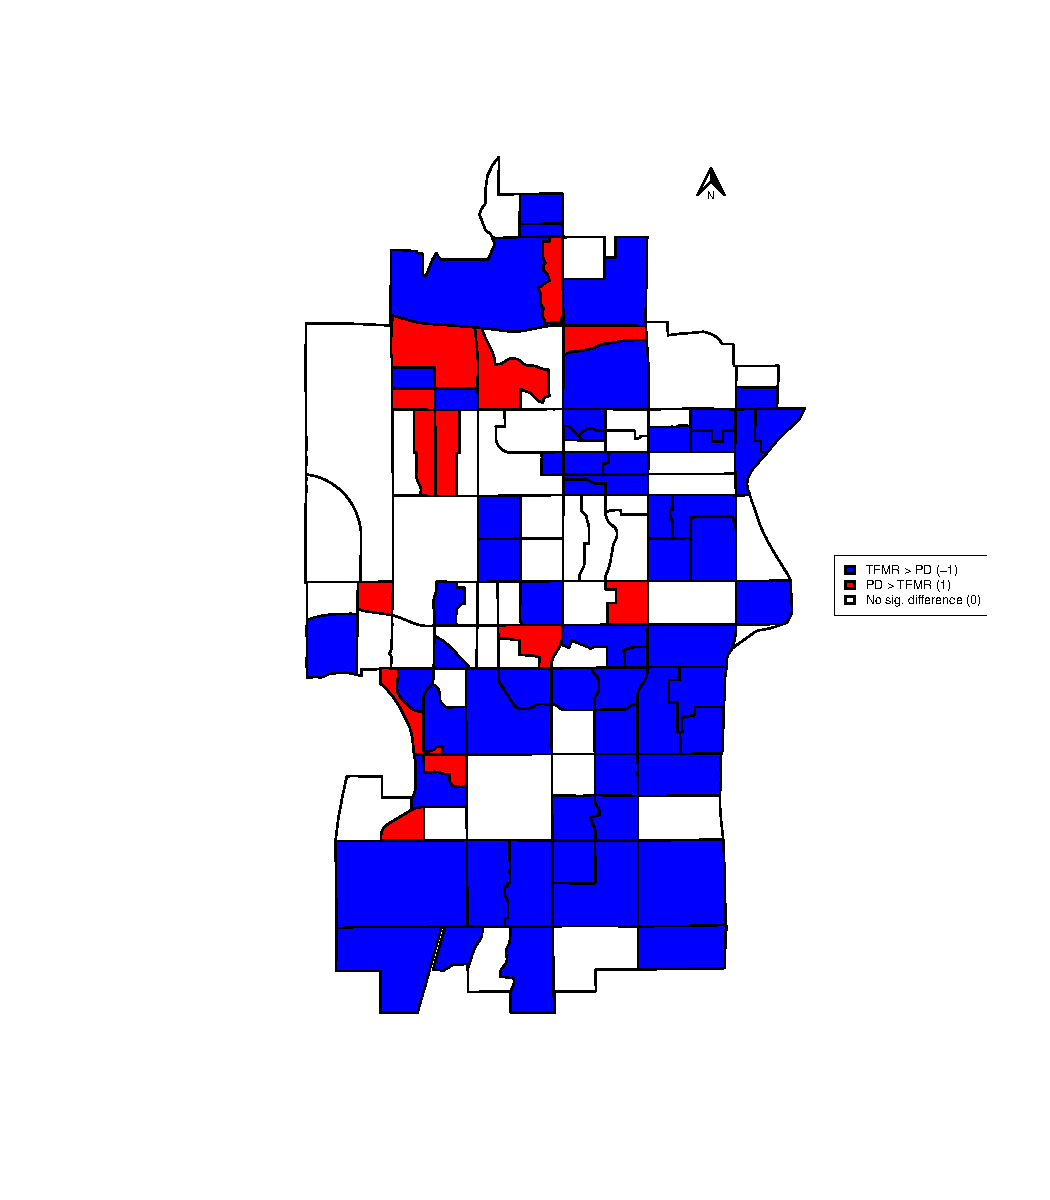
\includegraphics{figures/sppt-naloxone.pdf}
\end{figure}

\newpage

\begin{table}[htbp]\centering
\def\sym#1{\ifmmode^{#1}\else\(^{#1}\)\fi}
\caption{Mixed-effects Logistic Regression Models Predicting PD and TFMR first to Administer Naloxone}
\begin{adjustbox}{max width=\linewidth}\begin{tabular}{l*{2}{c}}
\toprule
                &\multicolumn{1}{c}{PD naloxone first}&\multicolumn{1}{c}{TFMR naloxone first}\\
\midrule
\emph{Independent variable}&                 &                 \\
Violent crime rate (per 1000)&0.997\sym{**} (0.001)        &1.001\sym{*} (0.001)        \\
\vspace{.05em} \\
Initial dispatch complaint (ref = Overdose/poisioning)&                 &                 \\
Health/medical related&0.684\sym{*} (0.104)        &1.326\sym{*} (0.182)        \\
Accidental injury&0.477 (0.502)        &0.770 (0.318)        \\
Public safety related&0.273 (0.282)        &0.519 (0.322)        \\
Mental health related&0.391\sym{**} (0.096)        &1.998\sym{**} (0.365)        \\
Other           &0.649\sym{**} (0.108)        &2.948\sym{**} (0.473)        \\
\vspace{.05em} \\
Female          &0.774 (0.127)        &1.126 (0.123)        \\
\vspace{.05em} \\
\emph{Block group predictors}&                 &                 \\
Violent crime spatial lag&1.008 (0.006)        &0.997 (0.004)        \\
Drug offense rate (per 1000)&1.007\sym{**} (0.002)        &0.994\sym{**} (0.002)        \\
Drug offense spatial lag&0.995 (0.007)        &1.005 (0.006)        \\
Opioid OD rate logged&0.937 (0.096)        &1.029 (0.087)        \\
Opioid OD spatial lag&0.996 (0.007)        &0.999 (0.006)        \\
\% Unemployed   &0.993 (0.012)        &0.999 (0.005)        \\
\% Residential land&1.001 (0.003)        &1.003 (0.002)        \\
\% Owner occupied units&0.978\sym{*} (0.009)        &0.995 (0.006)        \\
\% White        &1.012 (0.008)        &0.997 (0.005)        \\
\% Black        &1.025\sym{**} (0.007)        &0.987 (0.007)        \\
\% Hispanic     &1.007 (0.008)        &0.996 (0.006)        \\
Constant        &0.098\sym{**} (0.074)        &0.683 (0.355)        \\
\midrule
Random intercept&1.000\sym{**} (0.000)        &1.000 (0.000)        \\
\midrule
Observations    &     1,994        &     1,994        \\
Block groups    &  115        &  115        \\
AIC             & 1645.796        & 2464.457        \\
BIC             & 1830.527        & 2649.188        \\
\bottomrule
\multicolumn{3}{p{16cm}}{\footnotesize Exponentiated coefficients displayed. Clustered standard errors in parentheses. Month and year fixed effects included but not shown. Mean VIF value = 2.46, single highest VIF value = 7.49.}\\
\multicolumn{3}{l}{\footnotesize \sym{*} \(p<0.05\), \sym{**} \(p<0.01\), \sym{**} \(p<0.001\)}\\
\end{tabular} \end{adjustbox}
\end{table}


\newpage

\begin{table}[htbp]\centering
\def\sym#1{\ifmmode^{#1}\else\(^{#1}\)\fi}
\caption{Mixed-effects Logistic Regression Models Predicting PD and TFMR First to Administer Naloxone: PD and TFMR only}
\begin{adjustbox}{max width=\linewidth}\begin{tabular}{l*{2}{D{.}{.}{-1}}}
\toprule
                &\multicolumn{2}{c}{Police naloxone admin}\\\cmidrule(lr){2-3}
                &\multicolumn{1}{c}{(1)}        &\multicolumn{1}{c}{(2)}        \\
\midrule
\emph{Independent variable}&                 &                 \\
Violent crime rate (per 1000)&                 &0.995\sym{**} (0.001)        \\
\vspace{.05em} \\
Initial dispatch complaint (ref = Overdose/poisioning)&                 &                 \\
Health/medical related&                 &0.659\sym{*} (0.135)        \\
Accidental injury&                 &0.932 (1.005)        \\
Public safety related&                 &0.280 (0.193)        \\
Mental health related&                 &0.243\sym{**} (0.069)        \\
Other           &                 &0.347\sym{**} (0.072)        \\
\vspace{.05em} \\
Female          &                 &0.779 (0.149)        \\
\vspace{.05em} \\
Age range (ref = Aged 20 - 29)&                 &                 \\
Younger than 20 &                 &0.786 (0.279)        \\
Aged 30 - 39    &                 &0.881 (0.200)        \\
Aged 40 - 59    &                 &0.454\sym{**} (0.100)        \\
Aged 60 - 99    &                 &0.272\sym{**} (0.116)        \\
\vspace{.05em} \\
\emph{Block group predictors}&                 &                 \\
Violent crime spatial lag&                 &1.011 (0.007)        \\
Drug offense rate (per 1000)&                 &1.013\sym{**} (0.002)        \\
Drug offense spatial lag&                 &0.985\sym{*} (0.008)        \\
Opioid OD rate logged&                 &0.994 (0.149)        \\
Opioid OD spatial lag&                 &1.000 (0.001)        \\
Disadvantage&                 &1.079 (0.104)        \\
\% Residential land&                 &0.995 (0.003)        \\
\% Owner occupied units&                 &0.978 (0.013)        \\
\% White        &                 &1.024\sym{*} (0.011)        \\
\% Black        &                 &1.036\sym{**} (0.012)        \\
\% Hispanic     &                 &1.013 (0.010)        \\
Constant        &0.409\sym{**} (0.036)        &0.234 (0.263)        \\
\midrule
Random intercept&1.073 (0.067)        &1.000 (0.000)        \\
\midrule
Observations    &      955        &      891        \\
Block groups    &  112            &  106        \\
AIC             & 1170.921        & 1060.195        \\
BIC             & 1180.644        & 1381.282        \\
\bottomrule
\multicolumn{3}{p{20cm}}{\footnotesize Exponentiated coefficients; Clustered standard errors in parentheses; Day of month, month, and year fixed effects included but not shown; Mean VIF value = 2.30, single highest VIF value = 9.95. Reference group is now TFMR administering first -- Not all other observations.}\\
\multicolumn{3}{l}{\footnotesize \sym{*} \(p<0.05\), \sym{**} \(p<0.01\), \sym{**} \(p<0.001\)}\\
\end{tabular} \end{adjustbox}
\end{table}


\newpage

\begin{figure}
    \caption{Coefficient Plot Predicting First to Administer Naloxone}
    \centering
    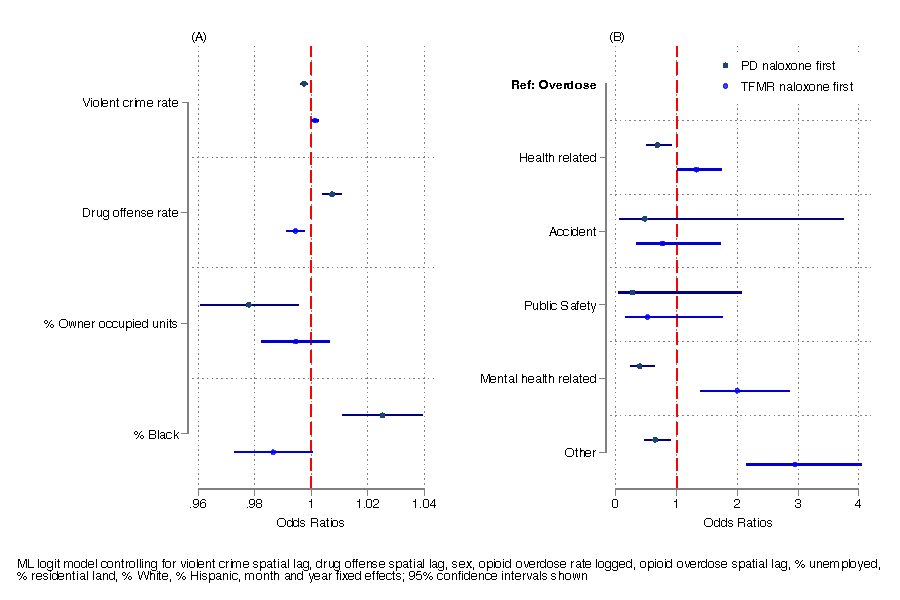
\includegraphics{figures/me-logit-coef-comb.pdf}
\end{figure} 


\newpage
\begin{figure}
    \caption{Coefficient Plot Predicting First to Administer Naloxone: PD and TFMR only}
    \centering
    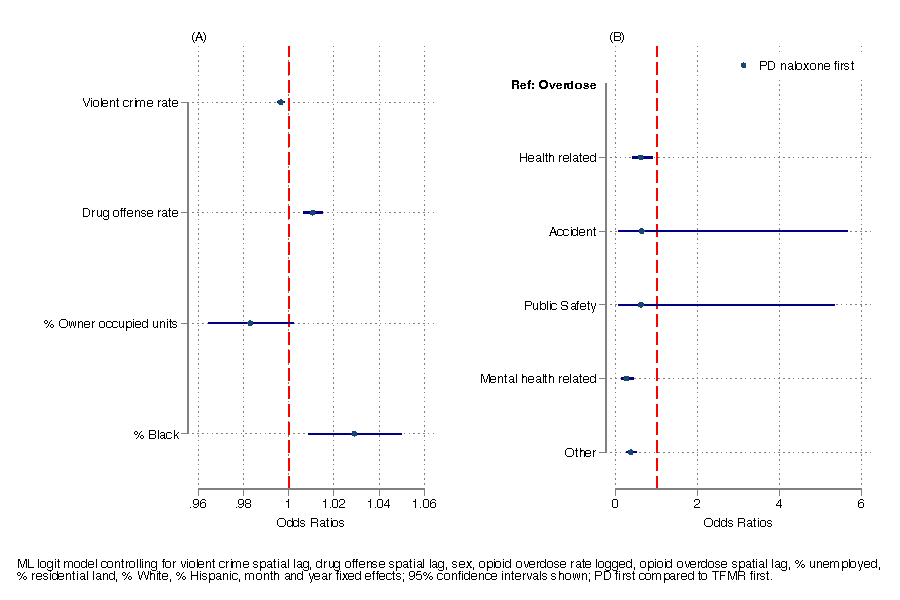
\includegraphics{figures/me-logit-coef-comb-sens.pdf}
\end{figure}

\newpage
\begin{table}[htbp] 
    \centering
    \def\sym#1{\ifmmode^{#1}\else\(^{#1}\)\fi}
    \caption{Modeling Spatial Variation in Naloxone Administration} % Title of the table
    \begin{adjustbox}{max width=\linewidth}
        \begin{tabular}{lc}
            \toprule
            \textbf{Potential Predictors} & \textbf{Predictors Modeled} \\ 
            \midrule
            \textbf{Systems-level}$^{a}$ & \\
            CAD system filtration of calls for service & \(\times\) \\
            \midrule
            \textbf{Community-level} & \\ 
            Violent crime rate & \checkmark \\ 
            Drug offense rate & \checkmark \\ 
            Opioid overdose rate & \checkmark \\ 
            Socioeconomic status & \checkmark \\ 
            Racial demographics & \checkmark \\
            Residential land use & \checkmark \\
            Total call volume: Police & \(\times\) \\
            Total call volume: Fire/EMS & \(\times\) \\
            Naloxone availability & \(\times\) \\ 
            Drug market shifts & \(\times\) \\
            \midrule
            \textbf{Agency-level}$^{b}$ & \\
            Staffing levels & \(\times\) \\
            Variation in deployment of resources & \(\times\) \\
            \midrule
            \textbf{Incident-level} & \\
            Initial call for service description & \checkmark \\
            Age of victim & \checkmark \\
            Sex of victim & \checkmark \\
            Location of incident (e.g., street, apartment, etc.) & \(\times\) \\
            Response time & \(\times\) \\
            Race of victim & \(\times\) \\
            Time of day & \(\times\) \\
            \midrule
            \textbf{Individual-level} & \\
            Experience and/or training to recognize an opioid overdose & \(\times\) \\
            Personal biases towards drug use/naloxone & \(\times\) \\
            \bottomrule
            \multicolumn{2}{p{17cm}}{\footnotesize $^{a}$Dispatch systems vary in how PD and EMS/Fire are notified of calls for service (e.g., one system or two), this could drive some spatial variation; $^{b}$Agency-level predictors could be accounted for in the day-, month-, and year-fixed effects}\\
        \end{tabular} 
    \end{adjustbox}
\end{table}                     %   \include rather than \input for chapters
\chapter{Who is Fatigued? Examining Officer Attitudes Towards PWUOs, Naloxone, and Their Role in Responding to Opioid Overdoses}

\section{Introduction}

The opioid overdose crisis, one of the longest ongoing public health crises, worsened in recent years when opioid overdose fatalities eclipsed 80,000 \parencite{center_for_disease_control_and_prevention_national_2023}. Since the 1990s a host of policies and programs have been implemented to reduce opioid overdose fatalities. One of the most common state-level policies of the last couple decades has been the implementation of Naloxone Access Laws (NALs). Naloxone is an opioid antagonist that binds to opioid receptors blocking the opioid from latching to the receptors \parencite{lurigio_opioid_2018}. This allows for the individual experiencing the overdose to regain proper respiratory functioning. According to the Legislative Analysis and Public Policy Association (LAPPA), every state has some form of a NAL, although the components of the policy varies \parencite{legislative_analysis_and_public_policy_association_naloxone_2022}. Additionally, Good Samaritan Laws (GSLs) have been signed into law in 50 states (and D.C.) which generally provide immunity to those who overdose as well as those who aid in helping the individual who overdosed, although the language varies from state to state \parencite{west_good_2023}. With the expansion of naloxone accessibility and the medication's ability to reverse opioid overdoses, as well as the immunity provided by GSLs, police departments have been increasingly outfitting their officers with naloxone \parencite{lurigio_opioid_2018}. In addition to carrying naloxone, there been efforts to act on police officers' frequent interactions with people who use drugs (PWUDs) and have them involved in collaborative efforts with social outreach organizations to reduce opioid overdose fatalities \parencite{donnelly_law_2022, formica_characteristics_2021, yatsco_alternatives_2020}. There is empirical evidence that suggests outfitting officers with naloxone can reduce overdose fatalities \parencite{rando_intranasal_2015}. Likewise, collaborative approaches between police department and public health agencies have been found to be effective at reducing fatal opioid overdoses \parencite{donnelly_law_2022} although the empirical base is limited given this is a relatively new approach.

However, while police officers have generally positive views of naloxone, some research has found that officers develop negative attitudes towards PWUDs, people who use opioids (PWUOs), naloxone, and drug treatment modalities as they respond to more overdoses \parencite{carroll_knowledge_2020, murphy_police_2020, murphy_police_2021}. This has been described as a potential compassion fatigue effect, where officers lose empathy and develop negative attitudes after repeatedly being involved in traumatic incidents \parencite{figley_compassion_1995, figley_treating_2002}. Compassion fatigue is not confined to police work and has been highlighted across professional contexts \parencite{adams_compassion_2006}. Within the police context, the development of negative attitudes with increased overdose response has implications for their involvement in opioid related issues. If officers develop negative attitudes their support for treatment may subside and there is the potential that it produces more punitive responses, which could hinder any collaborative or public health focused approach towards drug use \parencite{winstanley_bell_2020}.

In this study I explore Tempe police officer's perceptions and attitudes towards naloxone, PWUDs/PWUOs, and their role in responding to opioid overdoses across multiple waves of surveys. Then, I examine the relationship between opioid overdose response frequency and officer's perceptions. The findings have implications for police involvement in opioid overdose responses and police training focused substance use, and PWUOs.

\section{Literature Review}
\subsection{Police attitudes towards naloxone and PWUDs}
The police have increasingly become involved in responding to opioid overdoses and administering naloxone to combat rising opioid overdose fatalities. In some cases, the police are involved in referral or diversion programs to meet opioid overdose survivors with the potential to engage with social services. Due to law enforcement frequently being the first point of contact for someone who overdoses and a shift towards a public health model in some localities \parencite{beletsky_police_2011, silverman_harmonizing_2012}, there is a potential for police officers to save lives and to act as a conduit to services. While officer attitudes towards these issues were unexplored previously, their increased role in the opioid overdose crisis has prompted research into this area.

Prior work has found that officers have generally favorable attitudes towards naloxone and their role in responding to overdoses \parencite{purviance_law_2017, wagner_training_2016, white_narcan_2021}. Officers have reported feeling a sense of helplessness on scene at an overdose without being equipped with naloxone \parencite{banta-green_police_2013, white_moving_2021}. One way to improve officers’ ability to effectively handle an overdose situation is to provide them with naloxone. In 2013, Deputy Director of the U.S. National Drug Control Policy emphasized the importance of law enforcement to carry naloxone \parencite{michael_botticelli_announcing_2013}. Additionally, The Bureau of Justice Assistance highlighted that in addition to the ability to save lives, naloxone provides an improvement to job satisfaction among police officers \parencite{bureau_of_justice_assistance_law_nodate}. Indeed, outfitting officers with a medication that reverses the effects of an overdose is generally viewed favorably among officers. Having naloxone is another tool to use in order to save someone's life \parencite{lloyd_its_2023}. Other research has noted that the police want to be able to effectively provide life-saving care to reverse the effects of an overdose indicating their desire to carrying naloxone \parencite{purviance_law_2017}. And the idea of collaboration with public health agencies to address drug use is viewed as a more effective approach than traditional methods in some jurisdictions \parencite{lloyd_its_2023}.

Police officers can effectively administer naloxone and are receptive to training \parencite{lloyd_its_2023, pourtaher_naloxone_2022, purviance_law_2017, wagner_training_2016}. Police officers have displayed confidence in handling overdose situations as well \parencite{purviance_law_2017, ray_police_2015}. \textcite{white_narcan_2021} show that the items measuring competence and confidence had statistically significant improvements between wave 1 and wave 2 surveys (e.g., prior to carrying naloxone and 6 months after). Officers reported that they were more likely to disagree that they needed more training, that they were concerned about making a mistake, and that they were fearful of being sued. Officers were more likely to agree that they can recognize signs of an overdose, able to deal effectively with an overdose, and able to perform the recovery position on an overdose victim. Other studies have also found that competence tends to improve following training modules or experience with naloxone \parencite{wagner_training_2016} 

In addition to confidence in handling opioid overdoses, police officers have displayed improved perceptions of risk compensation beliefs. Risk compensation beliefs refer to the idea that naloxone availability will be associated with riskier drug use because naloxone acts as a safety net and prevents fatal overdoses. For instance, a recent study indicates that officers believed that naloxone and syringe exchange programs can lead to further opioid use \parencite{reichert_police_2023}. In a separate study, \textcite{winograd_concerns_2019} show that following a training, police officers' risk compensation beliefs improved significantly, which suggests these perceptions may be malleable.

Other research has casted doubt on the role of the police as a collaborative entity in combating the opioid overdose crisis \parencite{carroll_police_2023}. Police officers are not immune from stigmatizing views of PWUOs. While officers may have generally positive views of naloxone and their role in saving lives, much like the general population they still have negative perceptions towards PWUOs \parencite{barry_stigma_2014, calabrese_opposition_2019}. Studies have found that officers tend to agree that those who overdose are to blame \parencite{beletsky_attitudes_2005, wagner_training_2016}, naloxone enables PWUOs to continue using \parencite{banta-green_police_2013, burris_stopping_2009, reichert_police_2023}, and that naloxone encourages riskier drug use \parencite{saunders_you_2019}. Some of the negative perceptions can be corrected through training \parencite{winograd_concerns_2019}. Though others have shown that some perceptions may be less amenable following training modules \parencite{wagner_training_2016}. Additionally, law enforcement involvement in overdose situations can lead to criminalizing PWUOs \parencite{lowder_twoyear_2020, van_der_meulen_thats_2021}. Criminalization is not only harmful for the overdose victim but can subsequently lead to a hesitancy to call 911 due to fear of a police response and potential arrest \parencite{bohnert_policing_2011}. If police officers are often the first point of contact for PWUOs, their attitudes towards PWUOs, and their perceived role in the opioid overdose crisis is an important consideration. The development of negative perceptions and/or attitudes towards PWUOs could influence their discretion at the scene of an overdose resulting in more punitive outcomes for PWUOs.

\subsection{Compassion fatigue}

In addition to general attitudes towards naloxone, PWUOs, and officers’ role in responding to opioid overdoses, previous work has found that with increased response to opioid overdoses officers’ attitudes towards naloxone PWUOs decline. This is suggestive of a compassion fatigue effect. Compassion fatigue refers to the negative effect of vicarious traumatization. That is, an individual in an occupation where they care for and interact with individuals who experience traumatic events (e.g., first responders, therapists, etc.) may be vicariously traumatized and over time may become less empathetic and develop pessimistic attitudes \parencite{adams_compassion_2006, figley_compassion_1995}. 

While qualitative work has highlighted this potential compassion fatigue effect among police officers and other first-responders \parencite{banta-green_police_2013, saunders_you_2019}, more recent work has explored this finding quantitatively. \textcite{carroll_knowledge_2020} finds that as the frequency of overdose response increases, attitudes towards their scale of ‘enforcement overdose response efforts’ decline. Specifically, those who reported responding more than 4 times per month to an overdose has a composite score of 6.84. For those who had not responded to an overdose, their composite score was 8.13 which indicates a higher level of agreement towards law enforcement overdose response efforts. 

Likewise, \textcite{murphy_police_2020} investigate the compassion fatigue hypothesis using both bivariate and multivariate analyses for a sample of police officers in Pennsylvania. Murphy and Russell’s findings support the notion that officers feel trained and want to be involved in responding to opioid overdoses. Yet, they find that officers have negative attitudes towards drug treatment and PWUDs and that these negative attitudes are related to frequency of overdose response and naloxone administrations. \textcite{murphy_police_2021} also find that increased overdose response and naloxone administrations were negatively associated with treatment oriented policies.

\section{Current Study}

I am interested in examining how officers’ attitudes have changed towards naloxone, their role in responding to opioid overdoses, and PWUOs over four waves of surveys. This broad interest is driven by the compassion fatigue literature that suggests officer attitudes may become more pessimistic, less empathetic, and less supportive of overdose response efforts as they respond to more opioid overdoses. To evaluate the compassion fatigue hypothesis, I investigate two research questions:

1) Are officers’ attitudes towards naloxone, their role in responding to opioid overdoses, and their perceptions of PWUOs changing over time? 

\begin{flushleft}
\(H1_a\): Officer's attitudes towards their role in responding to opioid overdoses, naloxone, and PWUOs will change over time.
\end{flushleft}

2) Is opioid overdose response frequency associated with officer attitudes towards their role in responding to opioid overdoses, naloxone, and PWUOs? 

\begin{flushleft}
\(H2_a\): Officer's attitudes towards naloxone, PWUOs, and their role in responding to opioid overdoses will have a relationship with opioid overdose response frequency.
\end{flushleft}

To answer these research questions, I use survey data that captures Tempe officers’ attitudes at different time points over a four-year period. To examine attitudinal change over time, I will employ unconditional linear growth models. To answer the second research question, I run pooled OLS regression models with wave fixed effects to explore how the frequency of opioid overdose response impacts officers’ attitudes.

\section{Methods}
\subsection{Setting}

Since 2020 the Tempe Police Department (TPD) has been involved in a collaborative effort with a social services organization – EMPACT – to reduce opioid overdose fatalities in Tempe, Arizona. This project, called the Tempe First-Responder Opioid Recovery Project, is funded by the Substance Abuse and Mental Health Services Administration (SAMHSA). The project trained and outfitted Tempe officers with naloxone in January of 2020 and created a 24/7 crisis hotline which officers contacted following an overdose incident to get in contact with a peer navigator (e.g., social outreach worker). Within days of the incident the peer navigator meets with the overdose survivor and their family/friends to provide information regarding potentially useful services (e.g., counseling, drug rehabilitation, housing information, transportation, etc.). Tempe officers have responded to more than 300 overdose incidents during the project. They have administered naloxone over 250 times in which it aided in a successful reversal of opioid overdose symptoms, and they have contacted the 24/7 crisis hotline approximately the same number of times. 

\subsection{Data}

The data for this study come from multiple waves of surveys administered throughout the duration of the Tempe ORP. The first wave of surveys was administered prior to the project in December of 2019 (n = 242). In October of 2020, the second wave of surveys was administered (n = 117). These two waves were the focus of our prior study looking at officers’ perceptions \parencite{white_narcan_2021}. The third wave was conducted in November of 2021 (n = 62) and the final wave was administered in March and April of 2023 (n = 109). The first three waves of surveys were administered electronically through Google Forms. Due to the decline in the response rate in wave 3, hard copy surveys were used for the fourth wave to improve our response rate.  I attended 10 patrol briefings with the project manager at TPD and handed out hard copy surveys to a total of 18 squads (111 officers). All four waves of surveys were voluntary and anonymous. The survey took approximately 12 to 15 minutes both electronically and hard copy. The surveys mostly comprised of true/false and Likert scale statements that are on a four-point scale (1 = strongly disagree, 4 = strongly agree). Additionally, all four surveys utilize the OOKS and OOAS scales \parencite{williams_development_2013} and the NaRRC-B scale \parencite{winograd_concerns_2019}. The survey also captured officer demographics.

\subsection{Dependent Variables}

I focus on three mean index measures: The role of the police,  naloxone related beliefs, and stigma towards PWUOs (see Appendix B.1 for more detail). The role of the police is captured by indexing four items, "I am glad to be carrying naloxone," "Tempe police officers should carry naloxone," "I feel better able to do my job carrying naloxone," and "Police should not respond to overdoses."\footnote{Police should not respond to overdoses is reverse coded.} The items produce a Cronbach's alpha that is above the conventional .70 threshold (\(\alpha = .774\)).

Naloxone related compensation beliefs is captured with five items, "People will use more if they have access to naloxone," "Users will be less likely to go to treatment due to naloxone," "Limit the number of naloxone administrations per person," "Naloxone enables PWUDs to continue their use," and "Providing naloxone means I condone opioid use." These items produce a Cronbach's alpha that is above the conventional .70 threshold (\(\alpha = .868\)).

To measure stigma towards PWUOs I index four items, "People who overdose need to learn a lesson," "People who overdose deserve life-threatening outcomes," "People who overdose are to blame," and "Overdose survivors should be arrested." The items produce a Cronbach's alpha that is just below the conventional threshold of .70 (\(\alpha = .692\)).

The reasons these measures are chosen as outcome variables are two-fold. First, these items measure the concepts of interest and are of particular importance if they do indeed change over time or are influenced by opioid overdose response frequency. Theoretically, compassion fatigue would impact officer's attitudes towards these items. For instance, a decline in empathy towards PWUOs may produce pessimistic attitudes towards this population. Secondly, prior work on this topic has used similar measures. \textcite{murphy_police_2020} use a few different items. To capture officer attitudes towards naloxone they provide the following statements in their survey instrument: “Increasing access and utilization of Narcan is a good solution to the opioid problem,” “Increasing access and utilization of Narcan provides individuals with a substance use disorder an excuse to continue their drug use,” and “There should be a limit on how often someone who overdoses be administered Narcan.” While \textcite{carroll_knowledge_2020} use a “OD response efforts scale” that contains five Likert scale items that correspond to a variety of overdose prevention efforts such as distribution of naloxone, the value of Good Samaritan Laws, and community based prevention training programs. Following both \textcite{murphy_police_2020} and \textcite{carroll_knowledge_2020}, I use similar outcome variables that may be influenced by compassion fatigue. 

\subsection{Independent Variable}

There are two primary independent variables in this study. For the first research question, the wave of the survey is the independent variable of interest (i.e., 1, 2, 3, 4). The wave of the survey is effectively a measure of time which allows for an examination of how time is associated with shifts in attitudes. For the second research question, opioid overdose response frequency is the independent variable of interest. This variable is measured on a five-point scale: “Never (0),” “Rarely (less than once per week) (1),” “Once per week (2),” “Once per shift (3),” and “Multiple times per shift (4).”

Control variables include whether the respondent is a patrol officer; reference category is non-patrol. Having ever administered naloxone is measured as a dummy variable. Sex is measured as a dummy variable; males are the reference category. Race is captured as Black, Hispanic, and Other, while the reference category is White non-Hispanic. Education is measured as a dummy variable that indicates if the respondent has received a college education which includes two-year, four-year, and advanced degrees; the reference category includes high school diploma or a GED, and some college. Time spent at the Tempe Police Department is represented as a series of dummy variables 1-2 years, 3-5 years, 6-10 years, 11+ years at the department; the reference category is less than one year at the department. I then control for competence at the scene of an overdose. This variable is measured on a four-point Likert scale from completely disagree (1) to completely agree (4). Specifically, this item states “I would be able to effectively deal with an overdose.” A dummy variable for having administered naloxone is included in the model as well. Lastly, I incorporate wave fixed effects to control for unobservable time invariant characteristics between the waves of the survey.

\subsection{Analytical Sample}

The final analytical sample is comprised of 527 observations. However, listwise deletion removes approximately 13\% of the sample in the pooled ordinary least squares (OLS) regression models.\footnote{Models 1 and 3 drop 62 observations (13\%), Model 2 drops 61 observations (12\%).} 

Tables 1 and 2 provide a breakdown of the sample descriptive statistics. I will focus on table 2 here to discuss the descriptive statistics across the waves.\footnote{Because the fourth survey was administered in-person at roll-call, the sample in the fourth wave is younger and more likely to be on patrol compared to the first three waves. I control for both of these variables in the main regression models and run sensitivity checks on a patrol only sample (see Appendix B.3).} Focusing on the independent variable, frequency of overdose response increased across the waves. Never having responded to an overdose declined from wave 1 (19\%) to wave 4 (7\%) while responding to an overdose once per week increased by approximately 8\%. The most common response across all four waves is less than once per week (40\%-47\%). Ever having administered naloxone increased across the waves from 2\% to 67\%. Additionally, respondents are predominately White (70\%-89\%), male (81\%-87\%), college educated (67\%-83\%), and have been at the Tempe Police Department for 11 or more years (32\%-70\%).

\subsection{Analytical Plan}

The analysis proceeds as follows. First, to descriptively examine the change in attitudes over time, I will use three unconditional linear growth models. These will provide estimates for how attitudes have changed across the multiple waves of surveys over the course of the project. Then, to examine the relationship between opioid overdose response frequency and officer attitudes, I run three pooled OLS regression models with wave fixed effects.

\subsubsection{Unconditional Linear Growth Models}

\[Y_t = \beta_0 + \beta_1 Wave_t + \epsilon_t \]

Where \(Y_t\) is the outcome of interest (Police role, stigma towards PWUOs, and naloxone related beliefs) at wave \(t\). \(\beta_0\) is the intercept of outcome \(Y\). \(\beta_1\) is the coefficient for the primary independent variable -- waves of the survey. This represents the change in \(Y\) across the waves. Error is captured with the \(\epsilon_t\) term.

\subsubsection{Pooled OLS Regression Models}

\[Y = \beta_0 + \beta_1 OD response frequency + \beta_n X_n + \alpha_t + \epsilon \]

Where \(Y\) is the outcome of interest (Police role, stigma towards PWUOs, and naloxone related beliefs). \(\beta_0\) is the intercept of outcome \(Y\). \(\beta_1\) is the coefficient for the primary independent variable -- opioid overdose response frequency. \(\beta_n X_n\) represents the coefficients for a vector of covariates described above. \(\alpha_t\) represents wave fixed effects for wave \(t\). Error is captured with \(\epsilon\).

\section{Results}

Table 3 provides the results from the unconditional linear growth models. The results suggest that the wave of the survey is associated with changes in attitudes towards \textit{the role of the police} and \textit{stigma towards PWUOs}. Compared to wave 1, there was an increase of .152 (\(p < .1\)) in wave 3 and an increase of .372 (\(p < .01\)) in wave 4 for officer's support for their role in responding to opioid overdoses. Additionally, compared to wave 1, there was an increase of .249 (\(p < .01\)) in wave 3 and an increase of .155 (\(p < .05\)) in wave 4 for stigmatizing perceptions of PWUOs. Although these estimates are statistically significant, their standardized coefficients represent relatively small changes over time.\footnote{\textit{The role of the police} wave 3 standardized \(\beta\) = .08; wave 4 standardized \(\beta\) = .24. \textit{Stigma towards PWUOs} wave 3 standardized \(\beta\) = .14; wave 4 standardized \(\beta\) = .11.} Figure 1 provides a visualization of the unstandardized estimates across the waves of surveys. 

Table 4 presents the coefficients for the pooled OLS regression models. Here, I will restrict my discussion of the results by focusing on the primary independent variable of interest \parencite{keele_causal_2020}. The primary independent variable - opioid overdose response frequency - is not associated with any of the outcomes of interest. I will discuss this finding and other variables' relationships in more detail below. 

\section{Discussion}

In the present study I investigate the compassion fatigue hypothesis within the context of police responding to opioid overdoses using two approaches. First, the unconditional linear growth models provide mixed support for the first hypothesis. Officers' perceptions of \textit{the role of the police} and \textit{stigma towards PWUOs} did change over time. \textit{Perceptions of naloxone} did not change over time. Like previous work in this area, police officers generally had a positive view of naloxone and their role in saving lives \parencite{white_narcan_2021, pourtaher_naloxone_2022, reichert_police_2023}. The increased support for their role in responding to opioid overdoses may be related to the effectiveness of naloxone \parencite{white_leveraging_2022} or the effective working relationship with EMPACT, a social service organization who engages in post-overdose outreach with officers from the department \parencite{white_moving_2021}. Interestingly, the largest increase in officer attitudes towards their role in responding to overdoses is accompanied by a compositional change in the sample for wave 4. Respondents in this wave are younger, less likely to have a college degree, and more likely to be a patrol officer. Thus, they are most likely to be responding to opioid overdoses. Other work has demonstrated negative relationships between these covariates and officer attitudes towards opioid related issues \parencite{kruis_police_2020, reichert_police_2023}.

On the other hand, \textit{stigma of PWUOs} increases over time. Although data limitations prevent me from exploring this finding further, it is worth mentioning that over the course of the project the percentage of individuals who were homeless and received naloxone from Tempe police officers increased from 13\% in year one to 45\% in the final year of the project. The extent to which this trend contributed to an increase in stigmatizing views of PWUOs is unknown but there is evidence to suggest that officers who view PWUOs as unemployed or from a lower social class may perceive them to be more dangerous \parencite{kruis_police_2020}.

Second, I examine the relationship between opioid overdose response frequency and officer perceptions. Opioid overdose response frequency was not associated with any of the outcomes of interest. This suggests that opioid overdose exposure was not associated with improved or diminished attitudes towards the police role, naloxone, or stigma towards PWUOs. This finding holds true in a sensitivity check on a patrol only sample as well (see Appendix B.3). This finding runs counter to prior work that has reported an association between opioid response frequency and increased negative attitudes/perceptions \parencite{carroll_knowledge_2020, murphy_police_2020, murphy_police_2021}. It may be the case that Tempe officers have bought in to the role of responding to overdoses and administering naloxone. Prior to the first survey Tempe police officers did not have naloxone. \textcite{white_moving_2021} show that some officers felt a sense of futility when on scene at an overdose without naloxone, similar to studies in other jurisdictions, which has been found in other jurisdictions \parencite{smiley-mcdonald_perspectives_2022}. Having naloxone may be viewed as a tool that officers are able to quickly and easily use to save lives \parencite{lloyd_its_2023}. 

There were some covariate associations that are worth mentioning. Ever having administered naloxone was associated with an increase in support for officers' role in responding to opioid overdoses. Additionally, females were less likely to develop negative attitudes towards PWUOs. Similar to the analysis of the first two waves of surveys \parencite{white_narcan_2021}, those with a college degree and those who had been at the department longer (2-5, 6-10, and 11+ years) had negative attitudes towards the police role in opioid overdoses. These findings are counter to some of the findings in prior work, particularly for education \parencite{jorgensen_badges_2018}. Lastly, those who had higher levels of competence in handling an overdose were more likely to endorse the police role in opioid overdoses but also developed negative attitudes towards PWUOs. 

\subsection{Limitations}
The present study offers an analysis of the perspectives of Tempe police officers over the span of approximately 4 years. However, there are limitations that should be discussed. First, these attitudes are likely not generalizable to other jurisdictions. The Tempe Police Department is known for its focus on evidence-based practices. Over the last decade, they have participated in multiple research projects, including two randomized controlled trials (evaluating body-worn cameras and de-escalation training). The generally positive views from the first two ORP survey waves may be a product of the culture at Tempe PD \parencite{white_narcan_2021}. Second, the last wave of data used in the analysis come from in-person, hard copy administered surveys that were completed in tandem with “Narcan life-saving awards” being handed out by the project manager at Tempe PD. The first two survey waves were administered online. The context surrounding the administration of the final wave of surveys could increase the chance of social desirability impacting officers’ responses. Because the project manager, the awards, and I were present, this could have prompted the officers to respond more positively to survey items. However, whether this occurred or to what extent is unknown. Third, the between-subjects design of this study only examines aggregate mean trends across waves. While this approach is informative, it is limiting in that I am unable to measure within-subject variance over time. Future studies that examine the compassion fatigue hypothesis should attempt to overcome this limitation by creating a panel dataset of officer attitudes. Lastly, an aspect of officers' perceptions that is not available for modeling in this chapter is where the officer is patrolling. It may be the case that certain characteristics of neighborhoods or beats impact officers' perceptions of PWUOs, naloxone, and their role in the opioid overdose crisis. Future research should investigate the role of place in influencing officer perceptions related to the opioid crisis. 

\subsection{Implications}
Some potential implications can be gleaned from the findings. On a practical note, for program implementation and sustainability, patrol-level officer buy-in is an essential ingredient to a successful program. In order to facilitate this buy-in, broad department culture and immediate supervisor perceptions of these issues is also likely to be an important factor \parencite{del_pozo_police_2024}. Tempe Police Department had an internal champion guiding training's and garnering support within the department. This could be a contributing factor to officers' positive views and increased agreement towards their role in responding to opioid overdoses over time. 

Additionally, updated training modules for officers that cover substance use and naloxone is likely to play an important role. Training's have been shown to combat opioid myths surrounding fentanyl \parencite{del_pozo_can_2021}. This could also be applied to improving officer perceptions of PWUOs, particularly concerning stigmatizing views \parencite{winograd_concerns_2019}. If stigmatizing perceptions are associated with an increase in punitive outcomes, more harm will be created \parencite{binswanger_clinical_2016, ray_spatiotemporal_2023} and public-health approach to getting PWUOs in contact with potentially useful services will be hindered. The importance of training's and immediate supervisors are quite relevant here \parencite{del_pozo_police_2024}.  

\section{Conclusion}

The increased level of agreement with respect to the police role in opioid overdoses is likely due to a variety of factors including department culture, the effectiveness of naloxone, and the collaborative relationship between TPD and EMPACT \parencite{white_narcan_2021, white_moving_2021}. Tempe officers seem to buy-in to their role of carrying and administering naloxone. Regarding the increased stigma towards PWUOs, reintroducing training's focused on substance use should be offered to officers to provide more information related to opioids, naloxone, and PWUOs. 


\pagebreak
% table headers
% descriptive stats
\begin{table}[htbp]\centering
\def\sym#1{\ifmmode^{#1}\else\(^{#1}\)\fi}
\caption{\centering Summary Statistics}
\begin{tabular}{l*{1}{cccc}}
\toprule
                &     Mean&       SD&      Min&      Max\\
\midrule
\emph{Dependent Variables}&         &         &         &         \\
Role of the police&     2.98&     0.63&     1.00&     4.00\\
Naloxone related beliefs&     2.21&     0.56&     1.00&     4.00\\
Stigma towards PWUOs&     2.38&     0.59&     1.00&     4.00\\
\emph{OD Response Frequency}&         &         &         &         \\
Never           &     0.15&     0.36&     0.00&     1.00\\
Rarely (less than once per week)&     0.45&     0.50&     0.00&     1.00\\
Once per week   &     0.32&     0.47&     0.00&     1.00\\
Once per shift  &     0.05&     0.22&     0.00&     1.00\\
Multiple times per shift&     0.02&     0.13&     0.00&     1.00\\
\vspace{0.1em} \emph{Control Variables}&         &         &         &         \\
Ever administered naloxone&     0.25&     0.43&     0.00&     1.00\\
Patrol          &     0.57&     0.50&     0.00&     1.00\\
Female          &     0.16&     0.37&     0.00&     1.00\\
White           &     0.77&     0.42&     0.00&     1.00\\
Black           &     0.04&     0.19&     0.00&     1.00\\
Hispanic        &     0.14&     0.35&     0.00&     1.00\\
Other           &     0.05&     0.21&     0.00&     1.00\\
College degree  &     0.77&     0.42&     0.00&     1.00\\
Competence at an overdose&     2.94&     0.79&     1.00&     4.00\\
\emp{Time at Tempe PD}&         &         &         &         \\
Less than 1 year&     0.05&     0.22&     0.00&     1.00\\
1-2 years       &     0.07&     0.26&     0.00&     1.00\\
2-5 years       &     0.15&     0.36&     0.00&     1.00\\
6-10 years      &     0.15&     0.36&     0.00&     1.00\\
11+ years       &     0.58&     0.49&     0.00&     1.00\\
\bottomrule
\multicolumn{5}{l}{\footnotesize n = 527}\\
\end{tabular}
\end{table}


% descriptive stats by wave
% fix sd space in wave 4
\begin{landscape}
\begin{table}[htbp]\centering
\def\sym#1{\ifmmode^{#1}\else\(^{#1}\)\fi}
\caption{\centering Summary Statistics by Wave}
\begin{tabular}{l*{4}{cc}}
\hline\hline
                &        1&         &        2&         &        3&         &        4&         \\
\hline
\emph{Dependent Variables}&         &         &         &         &         &         &         &         \\
\hspace{0.25cm} Role of the police&     2.87&   (0.63)&     2.97&   (0.57)&     3.02&   (0.74)&     3.24&   (0.53)\\
\hspace{0.25cm} Naloxone related beliefs&     2.18&   (0.55)&     2.23&   (0.60)&     2.21&   (0.64)&     2.23&   (0.50)\\
\hspace{0.25cm} Stigma towards PWUOs&     2.30&   (0.56)&     2.39&   (0.60)&     2.55&   (0.62)&     2.45&   (0.60)\\
\emph{OD Response Frequency}&         &         &         &         &         &         &         &         \\
\hspace{0.25cm} Never&     0.19&   (0.39)&     0.17&   (0.38)&     0.13&   (0.34)&     0.07&   (0.26)\\
\hspace{0.25cm} Rarely (less than once per week)&     0.47&   (0.50)&     0.43&   (0.50)&     0.40&   (0.49)&     0.47&   (0.50)\\
\hspace{0.25cm} Once per week&     0.29&   (0.45)&     0.32&   (0.47)&     0.39&   (0.49)&     0.37&   (0.49)\\
\hspace{0.25cm} Once per shift&     0.04&   (0.19)&     0.07&   (0.25)&     0.06&   (0.25)&     0.06&   (0.23)\\
\hspace{0.25cm} Multiple times per shift&     0.01&   (0.11)&     0.02&   (0.13)&     0.02&   (0.13)&     0.03&   (0.17)\\
\vspace{0.1em} \emph{Control Variables}&         &         &         &         &         &         &         &         \\
\hspace{0.25cm} Ever administered naloxone&     0.02&   (0.14)&     0.22&   (0.41)&     0.45&   (0.50)&     0.67&   (0.47)\\
\hspace{0.25cm} Patrol&     0.47&   (0.50)&     0.53&   (0.50)&     0.53&   (0.50)&     0.85&   (0.36)\\
\hspace{0.25cm} Female&     0.16&   (0.37)&     0.14&   (0.34)&     0.18&   (0.38)&     0.19&   (0.39)\\
\hspace{0.25cm} White&     0.78&   (0.41)&     0.75&   (0.44)&     0.89&   (0.31)&     0.70&   (0.46)\\
\hspace{0.25cm} Black&     0.04&   (0.19)&     0.03&   (0.17)&     0.00&   (0.00)&     0.07&   (0.26)\\
\hspace{0.25cm} Hispanic&     0.13&   (0.34)&     0.17&   (0.37)&     0.07&   (0.26)&     0.18&   (0.38)\\
\hspace{0.25cm} Other&     0.05&   (0.21)&     0.06&   (0.23)&     0.04&   (0.19)&     0.05&   (0.22)\\
\hspace{0.25cm} College degree&     0.79&   (0.41)&     0.80&   (0.40)&     0.82&   (0.38)&     0.67&   (0.47)\\
\hspace{0.25cm} Competence at an overdose&     2.48&   (0.72)&     3.10&   (0.66)&     3.40&   (0.61)&     3.51&   (0.52)\\
\emp{Time at Tempe PD}&         &         &         &         &         &         &         &         \\
\hspace{0.25cm} Less than 1 year&     0.04&   (0.20)&     0.01&   (0.09)&     0.00&   (0.00)&     0.14&   (0.34)\\
\hspace{0.25cm} 1-2 years&     0.07&   (0.25)&     0.04&   (0.20)&     0.03&   (0.18)&     0.14&   (0.34)\\
\hspace{0.25cm} 2-5 years&     0.17&   (0.38)&     0.13&   (0.34)&     0.03&   (0.18)&     0.20&   (0.40)\\
\hspace{0.25cm} 6-10 years&     0.12&   (0.32)&     0.11&   (0.32)&     0.25&   (0.44)&     0.20&   (0.40)\\
\hspace{0.25cm} 11+ years&     0.60&   (0.49)&     0.70&   (0.46)&     0.68&   (0.47)&     0.32&   (0.47)\\
\hline\hline
\multicolumn{9}{l}{\footnotesize Mean, Standard deviation in parentheses; Wave 1 (n = 239), Wave 2 (n = 117), Wave 3 (n = 62), Wave 4 (n = 109)}\\
\end{tabular}
\end{table}

\end{landscape}


% growth model figure
% fix to include the note as the image note not the graph note
\begin{figure}
    \centering
    \caption{\centering Unconditional Linear Growth Models}
    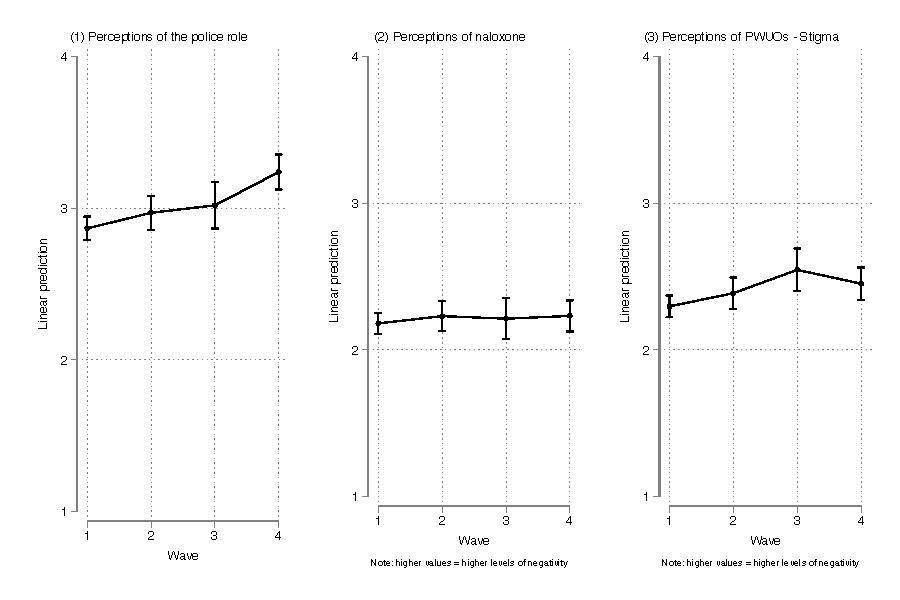
\includegraphics{figures/growth_models.pdf}
\end{figure}

% growth model coefficients table
\begin{table}[htbp]\centering
\def\sym#1{\ifmmode^{#1}\else\(^{#1}\)\fi}
\caption{\centering Unconditional Linear Growth Models}
\begin{tabular}{l*{3}{c}}
\toprule
                &\multicolumn{1}{c}{(1)}&\multicolumn{1}{c}{(2)}&\multicolumn{1}{c}{(3)}\\
                &\multicolumn{1}{c}{Role of the police}&\multicolumn{1}{c}{Naloxone related beliefs}&\multicolumn{1}{c}{Stigma towards PWUOs}\\
\midrule
Wave 2          &0.103 (0.069)        &0.050 (0.063)        &0.090 (0.066)        \\
\addlinespace
Wave 3          &0.152\sym{+} (0.087)        &0.032 (0.080)        &0.249\sym{**} (0.083)        \\
\addlinespace
Wave 4          &0.372\sym{**} (0.071)        &0.051 (0.065)        &0.155\sym{*} (0.067)        \\
\addlinespace
Constant        &2.867\sym{**} (0.040)        &2.181\sym{**} (0.036)        &2.297\sym{**} (0.038)        \\
\midrule
Observations    &      527        &      525        &      527        \\
\bottomrule
\multicolumn{4}{l}{\footnotesize Standard errors in parentheses}\\
\multicolumn{4}{l}{\footnotesize \sym{+} \(p<0.10\), \sym{*} \(p<0.05\), \sym{**} \(p<0.01\)}\\
\end{tabular}
\end{table}


% pooled reg models coefficients
% add note re robust se's in model (1) + reference categories: never responding to an overdose, never administered naloxone, White, male, less than a year at the department, in wave 1.
\begin{landscape}
   \begin{table}[htbp]\centering
\def\sym#1{\ifmmode^{#1}\else\(^{#1}\)\fi}
\caption{\centering Pooled OLS Regression Models}
\begin{tabular}{l*{3}{c}}
\toprule
                &\multicolumn{1}{c}{(1)}&\multicolumn{1}{c}{(2)}&\multicolumn{1}{c}{(3)}\\
                &\multicolumn{1}{c}{\hspace{0.25cm} Role of the police}&\multicolumn{1}{c}{\hspace{0.25cm} Naloxone related beliefs}&\multicolumn{1}{c}{\hspace{0.25cm} Stigma towards PWUOs}\\
\midrule
\emph{OD Response Frequency}&                  &                  &                  \\
\hspace{0.25cm} Rarely (less than once per week)&0.024 (0.082)         &-0.076 (0.076)         &-0.101 (0.078)         \\
\hspace{0.25cm} Once per week&0.000 (0.091)         &-0.005 (0.088)         &-0.069 (0.091)         \\
\hspace{0.25cm} Once per shift&0.034 (0.167)         &0.010 (0.133)         &-0.113 (0.138)         \\
\hspace{0.25cm} Multiple times per shift&-0.246 (0.262)         &0.042 (0.206)         &-0.008 (0.213)         \\
\vspace{0.1em} \emph{Control Variables}&                  &                  &                  \\
\hspace{0.25cm} Ever administered naloxone&0.190\sym{***} (0.068)         &-0.094 (0.076)         &-0.035 (0.078)         \\
\hspace{0.25cm} Patrol&-0.095 (0.066)         &0.081 (0.061)         &0.034 (0.063)         \\
\hspace{0.25cm} Black&0.220 (0.134)         &0.040 (0.134)         &-0.134 (0.139)         \\
\hspace{0.25cm} Hispanic&-0.001 (0.070)         &0.119 (0.073)         &-0.009 (0.075)         \\
\hspace{0.25cm} Other&-0.059 (0.119)         &0.096 (0.121)         &0.079 (0.125)         \\
\hspace{0.25cm} Female&0.070 (0.075)         &0.072 (0.069)         &-0.158\sym{**} (0.072)         \\
\hspace{0.25cm} College degree&-0.173\sym{***} (0.062)         &-0.054 (0.061)         &-0.030 (0.063)         \\
\hspace{0.25cm} Competence at an overdose&0.172\sym{***} (0.053)         &-0.042 (0.040)         &0.099\sym{**} (0.041)         \\
\emp{Time at Tempe PD}&                  &                  &                  \\
\hspace{0.25cm} 1-2 years&-0.137 (0.103)         &0.180 (0.145)         &-0.026 (0.150)         \\
\hspace{0.25cm} 2-5 years&-0.240\sym{**} (0.115)         &0.199 (0.133)         &0.001 (0.138)         \\
\hspace{0.25cm} 6-10 years&-0.419\sym{***} (0.114)         &0.303\sym{**} (0.133)         &0.028 (0.138)         \\
\hspace{0.25cm} 11+ years&-0.318\sym{***} (0.096)         &0.114 (0.121)         &-0.040 (0.125)         \\
\emp{Wave}      &                  &                  &                  \\
\hspace{0.25cm} Wave 2&0.012 (0.071)         &0.037 (0.070)         &0.053 (0.072)         \\
\hspace{0.25cm} Wave 3&0.046 (0.110)         &0.042 (0.094)         &0.119 (0.098)         \\
\hspace{0.25cm} Wave 4&0.051 (0.092)         &0.067 (0.090)         &0.066 (0.093)         \\
Constant        &2.901\sym{***} (0.179)         &2.130\sym{***} (0.164)         &2.153\sym{***} (0.170)         \\
\midrule
Observations    &      459         &      458         &      459         \\
\(R^{2}\)       &    0.164         &    0.050         &    0.051         \\
\bottomrule
\multicolumn{4}{l}{\footnotesize Standard errors in parentheses}\\
\multicolumn{4}{l}{\footnotesize \sym{*} \(p<0.10\), \sym{**} \(p<0.05\), \sym{***} \(p<0.01\)}\\
\end{tabular}
\end{table}
 
\end{landscape}

%Create appendix for tables of cronbach's alpha measurements on outcomes, linear growth model for patrol only 
\chapter{Collaborative Response to the Opioid Overdose Crisis: Evidence from a Quasi-Experimental Analysis}

\section{Introduction}
\section{Literature Review}
\subsection{}
\section{Methods}
\subsection{Setting}
\subsection{Data}
\subsection{Dependent Variables}
\subsection{Independent Variable}
\subsection{Analytical Sample}
\subsection{Analytical Plan}
\subsubsection{Segmented Generalized Least Squares (GLS) Regression Model}

\[Y = \beta_0 + \beta_1 TX + \beta_2 T + \beta_3 TS + \beta_4 POST + \beta_5 TXT + \beta_6 TXTS + \beta_7 TXPOST + \epsilon \]

Where \(Y\) is the outcome of interest (opioid overdose fatality rate per 100,000). \(\beta_0\) is the intercept of outcome \(Y\). \(\beta_1\) is the coefficient for a dummy treatment variable (=1 if group is in the treatment group). \(\beta_2\) represents the coefficient for time, which is a continuous measure. \(\beta_3\) is the coefficient for time since the intervention (=1 + \(n\) for months after treatment). \(\beta_4\) is the coefficient for the post-intervention period (=1 if in the post-treatment time period).  \(\beta_5\) corresponds to the coefficient of an interaction between the treatment dummy and time. \(\beta_6\) is the coefficient for an interaction between the treatment dummy and time since the intervention took place. Lastly, the \(\beta_7\) coefficient corresponds to an interaction between the treatment and post-intervention dummy variables. Error is captured by \(\epsilon\).

\section{Results}

\chapter{Conclusion}
                                        % Heading commands (in descending order):
                                        % \chapter
                                        % \section
                                        % \subsection
                                        % \subsubsection
                                        % \paragraph
                                        % \subparagraph
\iftoggle{sample}{%
  \chapter{This is a chapter-level heading}

\lipsum[1]

\section{This is the first section-level heading}

% Test single- and double-spacing around block quotes
Nam dui ligula, fringilla a, euismod sodales, sollicitudin vel, wisi. Morbi auctor
lorem non justo. Nam lacus libero, pretium at, lobortis vitae, ultricies et, tellus. Donec
aliquet, tortor sed accumsan bibendum, erat ligula aliquet magna, vitae ornare odio
metus a mi. Morbi ac orci et nisl hendrerit mollis. Suspendisse ut massa. Cras nec ante.
Pellentesque a nulla. Cum sociis natoque penatibus et magnis dis parturient montes,
nascetur ridiculus mus. Aliquam tincidunt urna. Nulla ullamcorper vestibulum turpis.
Pellentesque cursus luctus mauris.
\begin{quote}
Nulla malesuada porttitor diam. Donec felis erat, congue non, volutpat
at, tincidunt tristique, libero. Vivamus viverra fermentum felis. Donec
nonummy pellentesque ante. Phasellus adipiscing semper elit. Proin
fermentum massa ac quam. Sed diam turpis, molestie vitae, placerat
a, molestie nec, leo. Maecenas lacinia. Nam ipsum ligula, eleifend at,
accumsan nec, suscipit a, ipsum. Morbi blandit ligula feugiat magna.
Nunc eleifend consequat lorem. Sed lacinia nulla vitae enim. Pellentesque
tincidunt purus vel magna. Integer non enim. Praesent euismod nunc eu
purus. Donec bibendum quam in tellus. Nullam cursus pulvinar lectus.
Donec et mi. Nam vulputate metus eu enim. Vestibulum pellentesque
felis eu massa.
\end{quote}
Quisque ullamcorper placerat ipsum. Cras nibh. Morbi vel justo vitae lacus tincidunt
ultrices. Lorem ipsum dolor sit amet, consectetuer adipiscing elit. In hac habitasse
platea dictumst. Integer tempus convallis augue. Etiam facilisis. Nunc elementum
fermentum wisi. Aenean placerat. Ut imperdiet, enim sed gravida sollicitudin, felis
odio placerat quam, ac pulvinar elit purus eget enim. Nunc vitae tortor. Proin tempus
nibh sit amet nisl. Vivamus quis tortor vitae risus porta vehicula.

\subsection{This is the first sub-section-level heading}

% Make sure single- and double-spacing around blocks works with line breaks in the source
Nam dui ligula, fringilla a, euismod sodales, sollicitudin vel, wisi. Morbi auctor
lorem non justo. Nam lacus libero, pretium at, lobortis vitae, ultricies et, tellus. Donec
aliquet, tortor sed accumsan bibendum, erat ligula aliquet magna, vitae ornare odio
metus a mi. Morbi ac orci et nisl hendrerit mollis. Suspendisse ut massa. Cras nec ante.
Pellentesque a nulla. Cum sociis natoque penatibus et magnis dis parturient montes,
nascetur ridiculus mus. Aliquam tincidunt urna. Nulla ullamcorper vestibulum turpis.
Pellentesque cursus luctus mauris.

\begin{quote}
Nulla malesuada porttitor diam. Donec felis erat, congue non, volutpat
at, tincidunt tristique, libero. Vivamus viverra fermentum felis. Donec
nonummy pellentesque ante. Phasellus adipiscing semper elit. Proin
fermentum massa ac quam. Sed diam turpis, molestie vitae, placerat
a, molestie nec, leo. Maecenas lacinia. Nam ipsum ligula, eleifend at,
accumsan nec, suscipit a, ipsum. Morbi blandit ligula feugiat magna.
Nunc eleifend consequat lorem. Sed lacinia nulla vitae enim. Pellentesque
tincidunt purus vel magna. Integer non enim. Praesent euismod nunc eu
purus. Donec bibendum quam in tellus. Nullam cursus pulvinar lectus.
Donec et mi. Nam vulputate metus eu enim. Vestibulum pellentesque
felis eu massa.
\end{quote}

Quisque ullamcorper placerat ipsum. Cras nibh. Morbi vel justo vitae lacus tincidunt
ultrices. Lorem ipsum dolor sit amet, consectetuer adipiscing elit. In hac habitasse
platea dictumst. Integer tempus convallis augue. Etiam facilisis. Nunc elementum
fermentum wisi. Aenean placerat. Ut imperdiet, enim sed gravida sollicitudin, felis
odio placerat quam, ac pulvinar elit purus eget enim. Nunc vitae tortor. Proin tempus
nibh sit amet nisl. Vivamus quis tortor vitae risus porta vehicula.

\subsubsection{This is the first sub-sub-section-level heading}

\lipsum[1]

\paragraph{This is the first paragraph-level heading}

\lipsum[1]

\subparagraph{This is the first sub-paragraph-level heading}

\lipsum[1]

\section{Citation examples}

The contents of this section differ depending on the bibliography settings, specifically whether the `usebiblatex' toggle is set to `true' or `false'.
\iftoggle{usebiblatex}{%
  This sentence shows citation with biblatex \parencite{searchinger_world_2013}.
  This is another sentence showing citation with biblatex \parencite{pathak_rural_2007}.
}{%
  This sentence shows citation with natbib \citep{pathak_rural_2007}.
  This is another sentence showing citation with natbib \citep{searchinger_world_2013}.
}

\section{Footnote examples}

This is a sentence followed by a footnote.\footnote{Mauris ut leo. Cras viverra metus rhoncus sem. Nulla et lectus vestibulum urna fringilla ultrices. Phasellus eu tellus sit amet tortor gravida placerat. Integer sapien est, iaculis in, pretium quis, viverra ac, nunc. Praesent eget sem vel leo ultrices biben- dum. Aenean faucibus. Morbi dolor nulla, malesuada eu, pulvinar at, mollis ac, nulla.}
This is another sentence followed by a footnote.\footnote{Mauris ut leo. Cras viverra metus rhoncus sem. Nulla et lectus vestibulum urna fringilla ultrices. Phasellus eu tellus sit amet tortor gravida placerat. Integer sapien est, iaculis in, pretium quis, viverra ac, nunc. Praesent eget sem vel leo ultrices biben- dum. Aenean faucibus. Morbi dolor nulla, malesuada eu, pulvinar at, mollis ac, nulla.}

\section{Block quote example}

The following is a block quote:

\begin{quote}
\lipsum[1-2]
\end{quote}

\section{Endnote examples}

Endnotes appear in a separate section after chapters and before the reference list.
This is a sentence followed by a endnote.\pagenote{Mauris ut leo. Cras viverra metus rhoncus sem. Nulla et lectus vestibulum urna fringilla ultrices. Phasellus eu tellus sit amet tortor gravida placerat. Integer sapien est, iaculis in, pretium quis, viverra ac, nunc. Praesent eget sem vel leo ultrices biben- dum. Aenean faucibus. Morbi dolor nulla, malesuada eu, pulvinar at, mollis ac, nulla.}
This is another sentence followed by a endnote.\pagenote{Mauris ut leo. Cras viverra metus rhoncus sem. Nulla et lectus vestibulum urna fringilla ultrices. Phasellus eu tellus sit amet tortor gravida placerat. Integer sapien est, iaculis in, pretium quis, viverra ac, nunc. Praesent eget sem vel leo ultrices biben- dum. Aenean faucibus. Morbi dolor nulla, malesuada eu, pulvinar at, mollis ac, nulla.}
And here is a really long endnote to show formatting across several pages.\pagenote{\expandafter\lipsum[1-6]}

\section{Table example}

See table \ref{table\arabic{tablecounter}} for an example of a table.
Place macros inside captions using \string\macrocapwrap.
See table \ref{table\arabic{tablecounter}} for a demonstration.

\begin{table}[h] % Table float
\caption{Here is a table caption that is especially long to show what happens when it extends to more than one line in the table of contents}
\label{table\arabic{tablecounter}}
\begin{tabu}{l c c} \\ \hline
Column1 & Column2 & Column3 \\ \hline
Row1 & 2.0 & 3.0 \\
Row2 & 2.0 & 3.0 \\
Row3 & 7.0 & 8.0 \\ \hline
\end{tabu}
\legend{\emph{Source}: Here is a source note that is especially long to show what happens when it extends to more than one line.}
\legend{\emph{Note}: Here is a note that is especially long to show what happens when it extends to more than one line.}
\end{table}
\refstepcounter{tablecounter}

\begin{table}[h] % Table float
\caption{This table caption refers to another caption: see figure \macrocapwrap{\ref{figure1}} }
\label{table\arabic{tablecounter}}
\begin{tabu}{l c c} \\ \hline
Column1 & Column2 & Column3 \\ \hline
Row1 & 2.0 & 3.0 \\
Row2 & 2.0 & 3.0 \\
Row3 & 7.0 & 8.0 \\ \hline
\end{tabu}
\end{table}
\refstepcounter{tablecounter}

\section{Figure example}

See figure \ref{figure\arabic{figurecounter}} for an example of a figure.

\begin{figure}
\includegraphics[width=\maxwidth{\textwidth}]{src/sample/antidorcas.jpg}
\caption{Antidorcas marsupialis, male}
\label{figure\arabic{figurecounter}}
\legend{\emph{Source}: \iftoggle{usebiblatex}{\textcite{krishnappa_adult_2012}}{\citet{krishnappa_adult_2012}}}% See: https://upload.wikimedia.org/wikipedia/commons/8/89/Antidorcas_marsupialis%2C_male_%28Etosha%2C_2012%29.jpg
\legend{\emph{Note}: Here is a note that is especially long to show what happens when it extends to more than one line.}
\end{figure}
\refstepcounter{figurecounter}
\clearpage
\section{Math examples}

This section contains some math-heavy text adapted from \iftoggle{usebiblatex}{\textcite{dwilkins1995}}{\citet{dwilkins1995}}.
In non-relativistic wave mechanics, the wave function $\psi(\mathbf{r},t)$ of a particle satisfies the Schrödinger Wave Equation
%
\begin{equation}
 i\hbar\frac{\partial \psi}{\partial t}
  = \frac{-\hbar^2}{2m} \left(
    \frac{\partial^2}{\partial x^2}
    + \frac{\partial^2}{\partial y^2}
    + \frac{\partial^2}{\partial z^2}
  \right) \psi + V \psi.
\end{equation}
%
It is customary to normalize the wave equation by
demanding that
%
\begin{equation}
\int \!\!\! \int \!\!\! \int_{\textbf{R}^3}
      \left| \psi(\mathbf{r},0) \right|^2\,dx\,dy\,dz = 1.
\end{equation}
%
A simple calculation using the Schr\"{o}dinger wave
equation shows that
%
\begin{equation}
\frac{d}{dt} \int \!\!\! \int \!\!\! \int_{\textbf{R}^3}
      \left| \psi(\mathbf{r},t) \right|^2\,dx\,dy\,dz = 0,
\end{equation}
%
and hence
%
\begin{equation}
\int \!\!\! \int \!\!\! \int_{\textbf{R}^3}
      \left| \psi(\mathbf{r},t) \right|^2\,dx\,dy\,dz = 1
\end{equation}
%
for all times~$t$. If we normalize the wave function in this
way then, for any (measurable) subset~$V$ of $\textbf{R}^3$
and time~$t$,
%
\begin{equation}
\int \!\!\! \int \!\!\! \int_V
      \left| \psi(\mathbf{r},t) \right|^2\,dx\,dy\,dz
\end{equation}
%
represents the probability that the particle is to be found
within the region~$V$ at time~$t$.

\begin{table}[h] % Table float
\caption{This caption has math characters that remain lowercase: \relax\macrocapwrap{$\psi(\mathbf{r},t)$} }
\label{table\arabic{tablecounter}}
\begin{tabu}{l c c} \\ \hline
Column1 & Column2 & Column3 \\ \hline
Row1 & 2.0 & 3.0 \\
Row2 & 2.0 & 3.0 \\
Row3 & 7.0 & 8.0 \\ \hline
\end{tabu}
\end{table}
\refstepcounter{tablecounter}
%
}{}
%%%%%%%%%%%%%%%%%%%%%%%%%%%%%%%%%%%%%%%
% Back matter
%%%%%%%%%%%%%%%%%%%%%%%%%%%%%%%%%%%%%%%
\SingleSpacing                          % Back matter should be single spaced
\AfterEndEnvironment{table}{\SingleSpacing} % Reset these environments
\AfterEndEnvironment{figure}{\SingleSpacing}
\AfterEndEnvironment{quote}{\SingleSpacing}
\AfterEndEnvironment{quotation}{\SingleSpacing}

\edef\defaulttolerance{\the\tolerance}
\tolerance 500                          % Increase tolerance to prevent material extending into margins
\hbadness 500

\iftoggle{useendnotes}{%                % If you're using endnotes, output them here
  \setsecnumdepth{none}                 % No section numbering in end notes
  \bookmarksetup{startatroot}           % Make Notes appear at root level of PDF bookmarks
  \phantomsection%                      % Need for hyperref
  \addcontentsline{toc}{chapter}{%      % Add a chapter-level heading for
    \hspace{-\cftchapterindent}%        %  Notes to the ToC
    \notesname%
  }%
  \renewcommand*{\notedivision}{%
    \chapter*{\notesname}%
  }
  \printpagenotes                       % Output the notes
  \setsecnumdepth{all}%                 % Turn section numbering back on after printing
}{}

\bookmarksetup{startatroot}
\chapter*{\bibheading}                  % In the running text, use a chapter-level heading
                                        % for the bibliography section
\phantomsection
\addcontentsline{toc}{chapter}{%        % In the TOC, add a custom chapter-level heading
  \hspace{-\cftchapterindent}%          % that will be flush against the left margin
  \bibheading%
}
%\phantomsection
%\addtocontents{toc}%                    % Add this 'mark' to TOC so subsequent pages use
%  {\protect\markboth{\bibheading}{Page}}%   the bibliography heading (unlikely since
%                                        %   the appendices follow quickly)
\iftoggle{usebiblatex}{%                % Output the bibliography
  \printbibliography[heading=none]      % Using a 'biblatex' package; do not let
                                        %   'biblatex' output a heading
}{%
  \renewcommand\bibsection{}            % Do not let 'natbib' output a heading
  \bibliographystyle{\natbibstyle}      % Using 'natbib' to print bibliography
  \bibliography{\bibfilename}
}

\appendix                               % Indicate start of appendices
                                        % Appendices are considered 'mainmatter' in this
                                        %   documentclass
\tolerance \defaulttolerance            % Set tolerance back to default
\hbadness \defaulttolerance

\addtocontents{toc}{\protect%           % Only include appendix title in table of contents
  \setcounter{tocdepth}{0}}%            %   and omit sub-headings
\renewcommand*{\chapnamefont}%          % Reset font for 'Appendix' in chapter titles
    {\normalfont\MakeTextUppercase}
\makeatletter                           % Clear page after printing appendix title
  \renewcommand{\memendofchapterhook}%
  {%
    \clearpage
    \m@mindentafterchapter
    \@afterheading
  }
\makeatother

\phantomsection                         % Need '\phantomsection' to place hyperref
                                        %   bookmark more accurately
\addcontentsline{toc}{part}{Appendix}   %~Add "Appendix" to TOC here; comment out this
                                        %   line if you're not including appendices

\phantomsection                        %!This is the one part of the template that I
\addtocontents{toc}%                   %   could not get to work properly. After you
%{\protect\markboth{APPENDIX}{Page}}  %   start listing appendices in the TOC,
                                        %   subsequent TOC pages should use "APPENDIX in
                                        %   the header instead of "CHAPTER"; however,
                                        %   this code will make "APPENDIX" appear on the
                                        %   the same page that the *first* appendix
                                        %   appears on. This problem won't affect most
                                        %   people, but if it affects you, uncomment
                                        %   these lines and move them below where
                                        %   the appendices are listed. Keep moving these
                                        %   lines down and checking the output until
                                        %   the TOC headers appear correctly

\chapter{Investigating the Intersection of Policing, Place, and Opioids}

\begin{table}[htbp] \centering
\def\sym#1{\ifmmode^{#1}\else\(^{#1}\)\fi}
  \caption{Dispatch Type Coding} % Title of the table
  \begin{adjustbox}{max width=\linewidth}\begin{tabular}{p{6cm} p{10cm}}
    \toprule
     & Original Entry \\ 
    \midrule
    Overdose/Poisoning & Overdose/Poisoning/Ingestion \\
    \vspace{.05em} \\
    Health/Medical related & Abdominal pain; allergic reaction; Breathing problems; Chest pain; Cardiac arrest/Death; Choking; Convulsions/seizures; Diabetic problem; Headache; Eye problem/injury; Heat/cold exposure; Hemorrhage/laceration; Pregnancy/childbirth/miscarriage; Sick person; Stroke/CVA; Traumatic injury \\
    \vspace{.05em} \\
    Accidental injury & Falls; Burns/explosions; Animal bite \\
    \vspace{.05em} \\
    Public safety related & Stab/gunshot wound/penetrating trauma; Auto vs. pedestrian; Traffic/transportation incident; Assault \\
    \vspace{.05em} \\
    Mental health related & Altered mental status \\
    \vspace{.05em} \\
    Other & Medical alarm; Other; Unconscious/fainting/near-fainting; Unknown problem; Welfare check; Well person check \\
    \bottomrule
\end{tabular} \end{adjustbox}
\end{table}

\newpage

\begin{figure}
    \centering
    \caption{First to Administer Naloxone by Responder}
    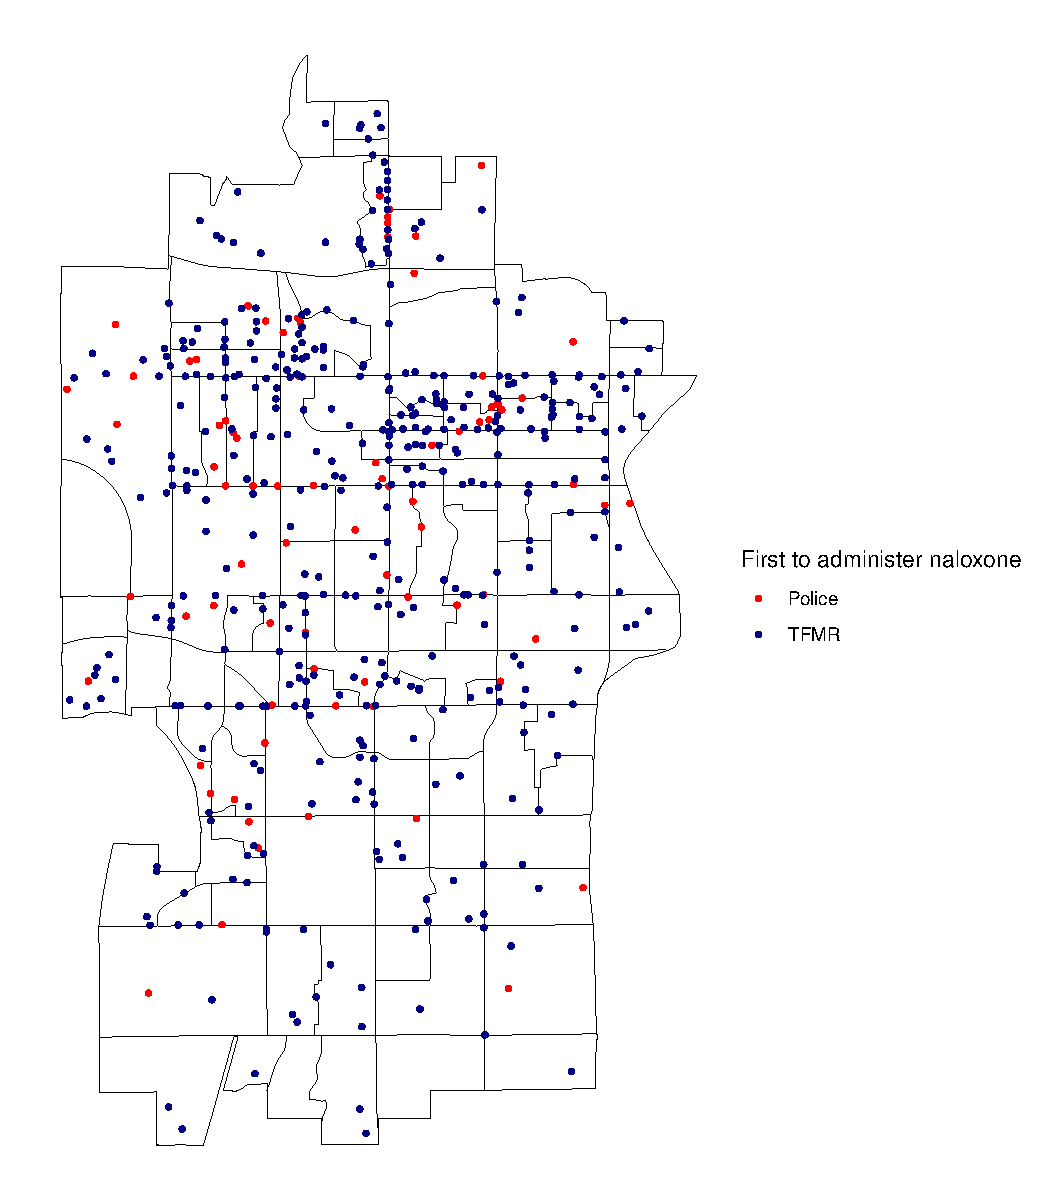
\includegraphics{figures/first-to-admin.pdf}
\end{figure}                       %~Insert your appendices here; I recommend to use
\chapter{Who is Fatigued? Examining Officer Attitudes Towards PWUOs, Naloxone, and Their Role in Responding to Opioid Overdoses}
\section{Latent Constructs - Cronbach's alpha}

\section{Subgroup Summary Statistics by Wave: Patrol only}
\begin{landscape}
\begin{table}[htbp]\centering
\def\sym#1{\ifmmode^{#1}\else\(^{#1}\)\fi}
\caption{\centering Summary Statistics by Wave: Patrol only}
\begin{tabular}{l*{4}{cc}}
\hline\hline
                &        1&         &        2&         &        3&         &        4&         \\
\hline
\emph{Dependent Variables}&         &         &         &         &         &         &         &         \\
\hspace{0.25cm} Role of the police&     2.79&   (0.71)&     3.04&   (0.58)&     2.97&   (0.75)&     3.28&   (0.49)\\
\hspace{0.25cm} Naloxone related beliefs&     2.27&   (0.54)&     2.19&   (0.53)&     2.39&   (0.67)&     2.18&   (0.45)\\
\hspace{0.25cm} Stigma towards PWUOs&     2.41&   (0.58)&     2.33&   (0.56)&     2.59&   (0.73)&     2.41&   (0.56)\\
\emph{OD Response Frequency}&         &         &         &         &         &         &         &         \\
\hspace{0.25cm} Never&     0.09&   (0.29)&     0.08&   (0.28)&     0.00&   (0.00)&     0.08&   (0.27)\\
\hspace{0.25cm} Rarely (less than once per week)&     0.32&   (0.47)&     0.31&   (0.46)&     0.28&   (0.46)&     0.42&   (0.50)\\
\hspace{0.25cm} Once per week&     0.49&   (0.50)&     0.46&   (0.50)&     0.59&   (0.50)&     0.41&   (0.49)\\
\hspace{0.25cm} Once per shift&     0.07&   (0.26)&     0.12&   (0.33)&     0.09&   (0.30)&     0.06&   (0.23)\\
\hspace{0.25cm} Multiple times per shift&     0.02&   (0.14)&     0.03&   (0.18)&     0.03&   (0.18)&     0.03&   (0.18)\\
\vspace{0.1em} \emph{Control Variables}&         &         &         &         &         &         &         &         \\
\hspace{0.25cm} Ever administered naloxone&     0.04&   (0.19)&     0.31&   (0.47)&     0.53&   (0.51)&     0.65&   (0.48)\\
\hspace{0.25cm} Female&     0.15&   (0.35)&     0.12&   (0.33)&     0.17&   (0.38)&     0.20&   (0.41)\\
\hspace{0.25cm} White&     0.74&   (0.44)&     0.71&   (0.46)&     0.86&   (0.35)&     0.70&   (0.46)\\
\hspace{0.25cm} Black&     0.06&   (0.24)&     0.05&   (0.23)&     0.00&   (0.00)&     0.07&   (0.26)\\
\hspace{0.25cm} Hispanic&     0.14&   (0.35)&     0.15&   (0.36)&     0.10&   (0.31)&     0.19&   (0.39)\\
\hspace{0.25cm} Other&     0.05&   (0.22)&     0.09&   (0.29)&     0.03&   (0.19)&     0.04&   (0.19)\\
\hspace{0.25cm} College degree&     0.78&   (0.41)&     0.81&   (0.39)&     0.77&   (0.43)&     0.66&   (0.48)\\
\hspace{0.25cm} Competence at an overdose&     2.57&   (0.74)&     3.22&   (0.62)&     3.47&   (0.51)&     3.55&   (0.50)\\
\emp{Time at Tempe PD}&         &         &         &         &         &         &         &         \\
\hspace{0.25cm} Less than 1 year&     0.07&   (0.25)&     0.02&   (0.13)&     0.00&   (0.00)&     0.16&   (0.37)\\
\hspace{0.25cm} 1-2 years&     0.12&   (0.33)&     0.08&   (0.28)&     0.06&   (0.25)&     0.16&   (0.37)\\
\hspace{0.25cm} 2-5 years&     0.18&   (0.39)&     0.10&   (0.30)&     0.00&   (0.00)&     0.19&   (0.39)\\
\hspace{0.25cm} 6-10 years&     0.11&   (0.32)&     0.12&   (0.33)&     0.22&   (0.42)&     0.19&   (0.39)\\
\hspace{0.25cm} 11+ years&     0.51&   (0.50)&     0.68&   (0.47)&     0.72&   (0.46)&     0.30&   (0.46)\\
\hline\hline
\end{tabular}
\end{table}

\end{landscape}

\section{Subgroup OLS regression models: Patrol only}
\begin{landscape}
\begin{table}[htbp]\centering
\def\sym#1{\ifmmode^{#1}\else\(^{#1}\)\fi}
\caption{\centering Pooled OLS Regression Models: Patrol only}
\begin{tabular}{l*{3}{c}}
\toprule
                &\multicolumn{1}{c}{(1)}&\multicolumn{1}{c}{(2)}&\multicolumn{1}{c}{(3)}\\
                &\multicolumn{1}{c}{Role of the police}&\multicolumn{1}{c}{Naloxone related beliefs}&\multicolumn{1}{c}{Stigma towards PWUOs}\\
\midrule
\emph{OD Response Frequency}&                  &                  &                  \\
Rarely (less than once per week)&-0.080 (0.138)         &-0.080 (0.130)         &-0.141 (0.143)         \\
Once per week   &-0.095 (0.139)         &0.043 (0.134)         &-0.093 (0.147)         \\
Once per shift  &-0.034 (0.209)         &0.087 (0.169)         &-0.206 (0.186)         \\
Multiple times per shift&-0.340 (0.290)         &0.007 (0.231)         &-0.117 (0.254)         \\
\vspace{0.1em} \emph{Control Variables}&                  &                  &                  \\
Ever administered naloxone&0.244\sym{**} (0.077)         &-0.101 (0.086)         &-0.061 (0.094)         \\
Black           &0.232 (0.154)         &0.006 (0.143)         &-0.118 (0.158)         \\
Hispanic        &-0.125 (0.096)         &0.080 (0.093)         &0.088 (0.102)         \\
Other           &-0.177 (0.146)         &0.151 (0.148)         &0.031 (0.163)         \\
Female          &0.146 (0.110)         &0.054 (0.089)         &-0.187 (0.098)         \\
College degree  &-0.231\sym{**} (0.077)         &0.127 (0.078)         &0.076 (0.086)         \\
Competence at an overdose&0.185\sym{*} (0.074)         &-0.028 (0.055)         &0.140\sym{*} (0.060)         \\
\emp{Time at Tempe PD}&                  &                  &                  \\
1-2 years       &-0.158 (0.118)         &0.149 (0.149)         &-0.049 (0.164)         \\
2-5 years       &-0.082 (0.134)         &0.156 (0.146)         &-0.041 (0.161)         \\
6-10 years      &-0.490\sym{***} (0.146)         &0.219 (0.149)         &0.004 (0.164)         \\
11+ years       &-0.355\sym{**} (0.117)         &0.109 (0.129)         &-0.068 (0.142)         \\
\emp{Wave}      &                  &                  &                  \\
Wave 2          &0.112 (0.109)         &-0.080 (0.097)         &-0.092 (0.106)         \\
Wave 3          &0.133 (0.133)         &0.068 (0.126)         &0.027 (0.139)         \\
Wave 4          &0.070 (0.116)         &0.001 (0.107)         &-0.050 (0.117)         \\
Constant        &2.864\sym{***} (0.243)         &2.080\sym{***} (0.210)         &2.118\sym{***} (0.231)         \\
\midrule
Observations    &      257         &      256         &      257         \\
\(R^{2}\)       &    0.278         &    0.073         &    0.059         \\
\bottomrule
\multicolumn{4}{l}{\footnotesize Standard errors in parentheses}\\
\multicolumn{4}{l}{\footnotesize \sym{*} \(p<0.05\), \sym{**} \(p<0.01\), \sym{***} \(p<0.001\)}\\
\end{tabular}
\end{table}

\end{landscape}                       %   \input rather than \include for appendices.
\chapter{Collaborative Response to the Opioid Overdose Crisis: Evidence from a Quasi-Experimental Analysis}

\begin{figure}
    \centering
    \caption{\centering First Difference Autocorrelation Test}
    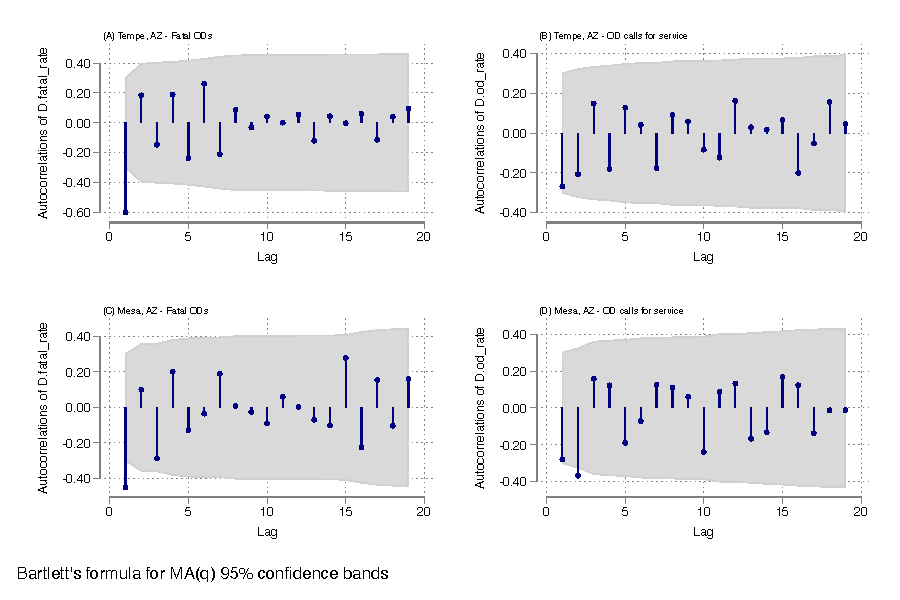
\includegraphics{figures/ac-lags-combined.pdf}
\end{figure}

\newpage

\begin{figure}
    \centering
    \caption{\centering Outliers: Pre-intervention Values}
    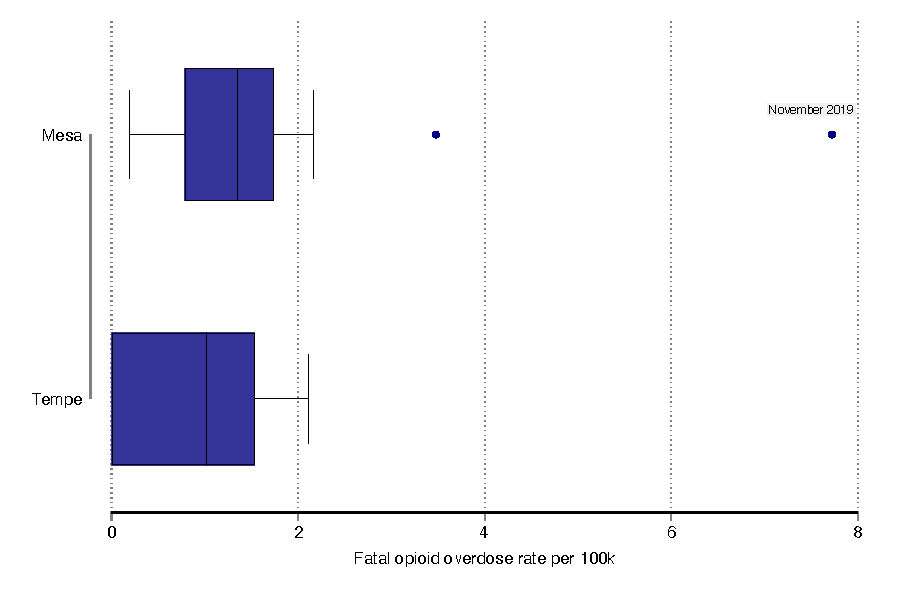
\includegraphics{figures/outlier.pdf}
\end{figure}

\newpage 




 % etc.                 %   All heading commands are the same as above,
                                         %   e.g., \chapter, \section, etc.
\iftoggle{sample}{%
  \input{src/sample/appendix}%
}{}

\backmatter                             % Start back matter according to documentclass
\makeatletter                           % Do not clear page after printing title for
  \renewcommand{\memendofchapterhook}%  %   biographical sketch
  {%
    \m@mindentafterchapter
    \@afterheading
  }
\makeatother

%\biographicalsketch{%                  %~Biographical Sketch is optional
%  \input{biography}%                   %<Enter the name of the .tex file containing your
%}%                                     %   biography or omit this line and type in
                                        %   your biography here (1 paragraph)
\end{document}
